%%
%% This is file `sample-acmlarge.tex',
%% generated with the docstrip utility.
%%
%% The original source files were:
%%
%% samples.dtx  (with options: `acmlarge')
%% 
%% IMPORTANT NOTICE:
%% 
%% For the copyright see the source file.
%% 
%% Any modified versions of this file must be renamed
%% with new filenames distinct from sample-acmlarge.tex.
%% 
%% For distribution of the original source see the terms
%% for copying and modification in the file samples.dtx.
%% 
%% This generated file may be distributed as long as the
%% original source files, as listed above, are part of the
%% same distribution. (The sources need not necessarily be
%% in the same archive or directory.)
%%
%%
%% Commands for TeXCount
%TC:macro \cite [option:text,text]
%TC:macro \citep [option:text,text]
%TC:macro \citet [option:text,text]
%TC:envir table 0 1
%TC:envir table* 0 1
%TC:envir tabular [ignore] word
%TC:envir displaymath 0 word
%TC:envir math 0 word
%TC:envir comment 0 0
%%
%%
%% The first command in your LaTeX source must be the \documentclass
%% command.
%%
%% For submission and review of your manuscript please change the
%% command to \documentclass[manuscript, screen, review]{acmart}.
%%
%% When submitting camera ready or to TAPS, please change the command
%% to \documentclass[sigconf]{acmart} or whichever template is required
%% for your publication.
%%
%%
%\documentclass[acmlarge]{acmart}
\documentclass[acmlarge,screen,nonacm]{acmart}

%%
%% \BibTeX command to typeset BibTeX logo in the docs
\AtBeginDocument{%
  \providecommand\BibTeX{{%
    Bib\TeX}}}

%% Rights management information.  This information is sent to you
%% when you complete the rights form.  These commands have SAMPLE
%% values in them; it is your responsibility as an author to replace
%% the commands and values with those provided to you when you
%% complete the rights form.
%\setcopyright{acmcopyright}
%\copyrightyear{2018}
%\acmYear{2018}
%\acmDOI{XXXXXXX.XXXXXXX}


%%
%% These commands are for a JOURNAL article.
%\acmJournal{POMACS}
%\acmVolume{37}
%\acmNumber{4}
%\acmArticle{111}
%\acmMonth{8}

%%
%% Submission ID.
%% Use this when submitting an article to a sponsored event. You'll
%% receive a unique submission ID from the organizers
%% of the event, and this ID should be used as the parameter to this command.
%%\acmSubmissionID{123-A56-BU3}

%%
%% For managing citations, it is recommended to use bibliography
%% files in BibTeX format.
%%
%% You can then either use BibTeX with the ACM-Reference-Format style,
%% or BibLaTeX with the acmnumeric or acmauthoryear sytles, that include
%% support for advanced citation of software artefact from the
%% biblatex-software package, also separately available on CTAN.
%%
%% Look at the sample-*-biblatex.tex files for templates showcasing
%% the biblatex styles.
%%

%%
%% The majority of ACM publications use numbered citations and
%% references.  The command \citestyle{authoryear} switches to the
%% "author year" style.
%%
%% If you are preparing content for an event
%% sponsored by ACM SIGGRAPH, you must use the "author year" style of
%% citations and references.
%% Uncommenting
%% the next command will enable that style.
%%\citestyle{acmauthoryear}

\usepackage{comment}
\usepackage{multirow}
\usepackage{amsmath,pifont}
\usepackage{booktabs}
\usepackage{rotating}
\usepackage{array}
\usepackage[para]{footmisc}
\newcolumntype{P}[2]{%
  >{\begin{turn}{#1}\begin{minipage}{#2}\footnotesize\raggedright\hspace{1pt}}c%
  <{\end{minipage}\end{turn}}%
}
\usepackage{tablefootnote}
\usepackage{xcolor}
\usepackage{colortbl}
\usepackage{longtable}
\usepackage{circledsteps}
\usepackage{diagbox}
\usepackage[ruled,linesnumbered]{algorithm2e}
\usepackage{tcolorbox}

\definecolor{Employer}{HTML}{18AFCC}
\definecolor{Platform}{HTML}{5F9099}
\definecolor{Worker}{HTML}{CC1865}

\newcommand{\cmark}{\ding{51}}
\newcommand{\xmark}{\ding{55}}

\settopmatter{printacmref=false}
%%
%% end of the preamble, start of the body of the document source.
\begin{document}

%%
%% The "title" command has an optional parameter,
%% allowing the author to define a "short title" to be used in page headers.
\title{Towards Open Federated Learning Platforms: Survey and Vision from Technical and Legal Perspectives}

%%
%% The "author" command and its associated commands are used to define
%% the authors and their affiliations.
%% Of note is the shared affiliation of the first two authors, and the
%% "authornote" and "authornotemark" commands
%% used to denote shared contribution to the research.

\author{Moming Duan}
\affiliation{%
  \institution{National University of Singapore}
  \city{Singapore}
  \country{Singapore}}
\email{moming@nus.edu.sg}

\author{Qinbin Li}
\affiliation{%
  \institution{University of California}
  \city{Berkeley}
  \country{USA}}
\email{qinbin@berkeley.edu}

\author{Linshan Jiang}
\affiliation{%
  \institution{National University of Singapore}
  \city{Singapore}
  \country{Singapore}}
\email{linshan@nus.edu.sg}

\author{Bingsheng He}
\affiliation{%
  \institution{National University of Singapore}
  \city{Singapore}
  \country{Singapore}}
\email{hebs@comp.nus.edu.sg}

%%
%% By default, the full list of authors will be used in the page
%% headers. Often, this list is too long, and will overlap
%% other information printed in the page headers. This command allows
%% the author to define a more concise list
%% of authors' names for this purpose.
\renewcommand{\shortauthors}{Duan et al.}

%%
%% The abstract is a short summary of the work to be presented in the
%% article.
\begin{abstract}
Traditional Federated Learning (FL) follows a server-domincated cooperation paradigm which narrows the application scenarios of FL and decreases the enthusiasm of data holders to participate.
To fully unleash the potential of FL, we advocate rethinking the design of current FL frameworks and extending it to a more generalized concept: Open Federated Learning Platforms, positioned as a crowdsourcing collaborative machine learning infrastructure for all Internet users. 
We propose two reciprocal cooperation frameworks for FL to achieve this: query-based FL and contract-based FL. 
In this survey, we conduct a comprehensive review of the feasibility of constructing an open FL platform from both technical and legal perspectives.
We begin by reviewing the definition of FL and summarizing its inherent limitations, including server-client coupling, low model reusability, and non-public.
In the query-based FL platform, which is an open model sharing and reusing platform empowered by the community for model mining, we explore a wide range of valuable topics, including the availability of up-to-date model repositories for model querying, legal compliance analysis between different model licenses, and copyright issues and intellectual property protection in model reusing.
In the contract-based FL platform, which is an opt-in model training network that allows multi-round communication and monetization, we explain how to select training frameworks according to microtasks and discuss the pros and cons of Decentralized Autonomous Organizations-based methods.
In particular, we introduce a novel taxonomy to streamline the analysis of model license compatibility in FL studies that involve batch model reusing methods, including combination, amalgamation, distillation, and generation. 
This taxonomy provides a systematic framework for identifying the corresponding clauses of licenses and facilitates the identification of potential legal implications and restrictions when reusing models.
Through this survey, we uncover the the current dilemmas faced by FL and advocate for the development of sustainable open FL platforms. 
We aim to provide guidance for establishing such platforms in the future, while identifying potential problems and challenges that need to be addressed.


%Then, for query-based FL, we survey the availability of online model repositories for neural networks in the context of model query.
%Furthermore, based on mainstream model licenses, we study the legal compliance between different licenses and provide guidelines for avoiding license conflicts.

\end{abstract}

%%
%% The code below is generated by the tool at http://dl.acm.org/ccs.cfm.
%% Please copy and paste the code instead of the example below.
%%
\begin{CCSXML}
<ccs2012>
 <concept>
  <concept_id>10010520.10010553.10010562</concept_id>
  <concept_desc>Computer systems organization~Embedded systems</concept_desc>
  <concept_significance>500</concept_significance>
 </concept>
 <concept>
  <concept_id>10010520.10010575.10010755</concept_id>
  <concept_desc>Computer systems organization~Redundancy</concept_desc>
  <concept_significance>300</concept_significance>
 </concept>
 <concept>
  <concept_id>10010520.10010553.10010554</concept_id>
  <concept_desc>Computer systems organization~Robotics</concept_desc>
  <concept_significance>100</concept_significance>
 </concept>
 <concept>
  <concept_id>10003033.10003083.10003095</concept_id>
  <concept_desc>Networks~Network reliability</concept_desc>
  <concept_significance>100</concept_significance>
 </concept>
</ccs2012>
\end{CCSXML}

%\ccsdesc[500]{Computer systems organization~Embedded systems}
%\ccsdesc[300]{Computer systems organization~Redundancy}
%\ccsdesc{Computer systems organization~Robotics}
%\ccsdesc[100]{Networks~Network reliability}

%%
%% Keywords. The author(s) should pick words that accurately describe
%% the work being presented. Separate the keywords with commas.
%\keywords{datasets, neural networks, gaze detection, text tagging}

%\received{20 February 2007}
%\received[revised]{12 March 2009}
%\received[accepted]{5 June 2009}

%%
%% This command processes the author and affiliation and title
%% information and builds the first part of the formatted document.
\maketitle

\section{Introduction}
Introduction:
Federated Learning~\cite{li2020federated}.

\subsection{Related Surveys}
In recent years, federated learning has become a buzzword in various fields, leading to the emergence of numerous FL studies.
These works can be classified into three primary categories: FL systems design, FL appllications and FL toolkits. Extensive surveys are available to summarized the advancement of federated learning, as shown in Table~\ref{table:surveys}.
The initial architectures and concepts for FL systems were summaried by Yang \textit{et al.}~\cite{yang2019federated}. 
They categorize FL into horizontal FL, vertical FL and federated transfer learning based on the distribution characteristics of data, 
which are written in IEEE Standard 3652.1-2020~\cite{yang2021white, IEEEstd3652}. 
Following this, an increasing number of surveys have emerged focusing on enhancing FL system design~\cite{li2020federated,aledhari2020federated, kairouz2021advances, zhang2021survey, li2021survey}. 
From the algorithmic perspective, personlized FL~\cite{kulkarni2020survey, tan2022towards} aims to learn personlized models for each client to address the challenge of statistical heterogeneity~\cite{ma2022state}.
Besides, the privacy-perserving computing platforms and model aggregation protocols for FL systems also been widely studied and sumaried by~\cite{liu2022privacy,el2022differential,yin2021comprehensive,lyu2020threats}.
Furthermore, many advanced FL architectures had been proposed, such as asynchronous~\cite{xu2021asynchronous}, decentralized and blockchain-based FL frameworks~\cite{nguyen2021federated, qu2022blockchain, zhu2022blockchain}.
Given that federated learning technologies enable collaboration among distributed participants in model training and decision-making, this capability holds great promise in a wide range of application scenarios.
For instance, multiple geogrphically distributed medical insitutions can enhace medication recommendation, drug-drug interaction prediction and medical image analysis in a collaborative manner without exchanging any sensitive data~\cite{xu2021federated, pfitzner2021federated, antunes2022federated, rieke2020future}. 
The massive real-time data generated by IoT devices in smart cities~\cite{zhang2022federated, ramu2022federated}, industries~\cite{boopalan2022fusion}, vehicles~\cite{du2020federated} has also sparked interest in exploring how FL technology can be used to deliver more advanced services such as intrusion detection, anomaly detection, fraud detection and network load prediction~\cite{agrawal2022federated, alazab2021federated, ghimire2022recent}.

As summarized in Table~\ref{table:surveys}, most surveys extensively discuss the challenges of efficiency, heterogeneity, privacy in FL systems design, with the surveys from blockchain fileds offering the most comprehensive review.
However, except for a few blockchain-based FL studies, most of the above surveys just present the same story from slightly different angles or backgrounds, i.e a server sets the model training task and delegate it to data holders to complete. 
This \textbf{server-domincated} cooperation framework is a narrow implementation of the FL systems.
Therefore, this survey aim to fill the gap by investigating and surveying the associated tenchnologies that support more open and inclusive cooperation frameworks in FL systems, where all entities (whether they own the data or not) can benefit from it. 
The challenges investigated in this survey are not listed in the Table~\ref{table:surveys}, to the best of our knowledge, this is the first survey that focuses on the cooperation frameworks of FL.
In the following section, we will differentiate this survey from other related concepts in the field of FL.

\begin{table}[]
    \footnotesize
    \caption{Summary of existing FL surveys, SYS denotes FL Systems Design, APP denotes FL Applications, SDC denotes Server-Dominated Cooperation frameworks.}
    \label{table:surveys}
    \begin{tabular}{|l|l|lllll|lll|}
    \hline
                       & \multicolumn{1}{c|}{} & \multicolumn{5}{c|}{Challenges}                                                                            & \multicolumn{3}{c|}{Contents}                            \\ \hline
                       Scenarios/Tasks &           FL Surveys            & \multicolumn{1}{l|}{Efficiency} & \multicolumn{1}{l|}{Heterogeneity} & \multicolumn{1}{l|}{Privacy} & \multicolumn{1}{l|}{Incentive} & Decentralized & \multicolumn{1}{l|}{SYS} & \multicolumn{1}{l|}{APP} & SDC \\ \hline
    \multirow{14}{*}{General} &      Yang \textit{et al.}~\cite{yang2019federated}         & \multicolumn{1}{c|}{ \checkmark } & \multicolumn{1}{c|}{\checkmark} & \multicolumn{1}{c|}{\checkmark} & \multicolumn{1}{c|}{\checkmark} & \multicolumn{1}{c|}{\checkmark}  & \multicolumn{1}{c|}{\checkmark} & \multicolumn{1}{c|}{\checkmark} & \multicolumn{1}{c|}{\checkmark}  \\ \cline{2-10}              
                        &   Li \textit{et al.} 2020~\cite{li2020federated}                    & \multicolumn{1}{c|}{\checkmark} & \multicolumn{1}{c|}{\checkmark} & \multicolumn{1}{c|}{\checkmark} & \multicolumn{1}{l|}{} & \multicolumn{1}{c|}{\checkmark} & \multicolumn{1}{c|}{\checkmark} & \multicolumn{1}{c|}{\checkmark} & \multicolumn{1}{c|}{\checkmark} \\ \cline{2-10} 
                        &   Zhang 2021\textit{et al.}~\cite{zhang2021survey}                    & \multicolumn{1}{c|}{\checkmark} & \multicolumn{1}{c|}{\checkmark} & \multicolumn{1}{c|}{\checkmark} & \multicolumn{1}{l|}{} &  & \multicolumn{1}{c|}{\checkmark} & \multicolumn{1}{c|}{\checkmark} & \multicolumn{1}{c|}{\checkmark} \\ \cline{2-10} 
                       &   Gupta \textit{et al.}~\cite{gupta2022survey}        & \multicolumn{1}{c|}{\checkmark} & \multicolumn{1}{c|}{\checkmark} & \multicolumn{1}{c|}{\checkmark} & \multicolumn{1}{l|}{} & \multicolumn{1}{c|}{\checkmark} & \multicolumn{1}{c|}{\checkmark} & \multicolumn{1}{c|}{\checkmark} & \multicolumn{1}{c|}{\checkmark} \\ \cline{2-10} 
                       &   Xu \textit{et al.}~\cite{xu2021asynchronous}                    & \multicolumn{1}{c|}{\checkmark} & \multicolumn{1}{c|}{\checkmark} & \multicolumn{1}{c|}{\checkmark} & \multicolumn{1}{l|}{} & \multicolumn{1}{c|}{\checkmark} & \multicolumn{1}{c|}{\checkmark} & \multicolumn{1}{c|}{\checkmark} & \multicolumn{1}{c|}{\checkmark} \\ \cline{2-10} 
                       &   Li \textit{et al.} 2021~\cite{li2021survey}        & \multicolumn{1}{c|}{\checkmark} & \multicolumn{1}{c|}{\checkmark} & \multicolumn{1}{c|}{\checkmark} & \multicolumn{1}{c|}{\checkmark} & \multicolumn{1}{c|}{\checkmark} & \multicolumn{1}{c|}{\checkmark} & \multicolumn{1}{c|}{\checkmark} & \multicolumn{1}{c|}{\checkmark} \\ \cline{2-10} 
                       &        El \textit{et al.}~\cite{el2022differential}               & \multicolumn{1}{l|}{} & \multicolumn{1}{l|}{} & \multicolumn{1}{c|}{\checkmark}& \multicolumn{1}{l|}{} & \multicolumn{1}{c|}{\checkmark} & \multicolumn{1}{c|}{\checkmark} & \multicolumn{1}{l|}{} & \multicolumn{1}{c|}{\checkmark} \\ \cline{2-10} 
                       &   Kulkarni \textit{et al.}~\cite{kulkarni2020survey}            & \multicolumn{1}{c|}{\checkmark} & \multicolumn{1}{c|}{\checkmark} & \multicolumn{1}{l|}{} & \multicolumn{1}{l|}{} &  & \multicolumn{1}{c|}{\checkmark} & \multicolumn{1}{l|}{} & \multicolumn{1}{c|}{\checkmark} \\ \cline{2-10} 
                       &  Liu \textit{et al.}\cite{liu2022privacy}             & \multicolumn{1}{c|}{\checkmark} & \multicolumn{1}{l|}{} & \multicolumn{1}{c|}{\checkmark} & \multicolumn{1}{l|}{} & \multicolumn{1}{c|}{\checkmark} & \multicolumn{1}{c|}{\checkmark} & \multicolumn{1}{l|}{} & \multicolumn{1}{c|}{\checkmark} \\ \cline{2-10} 
                       &    Tan \textit{et al.}~\cite{tan2022towards}     & \multicolumn{1}{l|}{} & \multicolumn{1}{c|}{\checkmark} & \multicolumn{1}{l|}{} & \multicolumn{1}{l|}{} &  & \multicolumn{1}{c|}{\checkmark} & \multicolumn{1}{l|}{} & \multicolumn{1}{c|}{\checkmark} \\ \cline{2-10} 
                       &           Zhu \textit{et al.} 2021~\cite{zhu2021federated}            & \multicolumn{1}{l|}{} & \multicolumn{1}{c|}{\checkmark} & \multicolumn{1}{l|}{} & \multicolumn{1}{l|}{} &  & \multicolumn{1}{c|}{\checkmark} & \multicolumn{1}{l|}{} & \multicolumn{1}{c|}{\checkmark} \\ \cline{2-10} 
                       &          Ma \textit{et al.}~\cite{ma2022state}            & \multicolumn{1}{c|}{\checkmark} & \multicolumn{1}{c|}{\checkmark} & \multicolumn{1}{c|}{\checkmark} & \multicolumn{1}{l|}{} &  & \multicolumn{1}{c|}{\checkmark} & \multicolumn{1}{l|}{} & \multicolumn{1}{c|}{\checkmark} \\ \cline{2-10} 
                       & Aledhari \textit{et al.}~\cite{aledhari2020federated}              & \multicolumn{1}{c|}{\checkmark} & \multicolumn{1}{c|}{\checkmark} & \multicolumn{1}{l|}{} & \multicolumn{1}{l|}{} &  & \multicolumn{1}{c|}{\checkmark} & \multicolumn{1}{c|}{\checkmark} & \multicolumn{1}{c|}{\checkmark} \\ \cline{2-10} 
                       &   Kairouz \textit{et al.}~\cite{kairouz2021advances}          & \multicolumn{1}{c|}{\checkmark} & \multicolumn{1}{c|}{\checkmark} & \multicolumn{1}{c|}{\checkmark} & \multicolumn{1}{c|}{\checkmark} & \multicolumn{1}{c|}{\checkmark} & \multicolumn{1}{c|}{\checkmark} & \multicolumn{1}{c|}{\checkmark} & \multicolumn{1}{c|}{\checkmark} \\ \cline{2-10} 
                       &      AbdulRahman \textit{et al.}~\cite{abdulrahman2020survey}   & \multicolumn{1}{c|}{\checkmark} & \multicolumn{1}{c|}{\checkmark} & \multicolumn{1}{c|}{\checkmark} & \multicolumn{1}{c|}{\checkmark} &  & \multicolumn{1}{c|}{\checkmark} & \multicolumn{1}{c|}{\checkmark} & \multicolumn{1}{c|}{\checkmark} \\ \cline{2-10} 
                       &    Lim \textit{et al.}~\cite{lim2020federated}       & \multicolumn{1}{c|}{\checkmark} & \multicolumn{1}{c|}{\checkmark} & \multicolumn{1}{c|}{\checkmark} & \multicolumn{1}{c|}{\checkmark} &  & \multicolumn{1}{c|}{\checkmark} & \multicolumn{1}{c|}{\checkmark} & \multicolumn{1}{c|}{\checkmark} \\ \hline
    \multirow{4}{*}{Healthcare}  &   Xu \textit{et al.}~\cite{xu2021federated}             & \multicolumn{1}{c|}{\checkmark} & \multicolumn{1}{c|}{\checkmark} & \multicolumn{1}{c|}{\checkmark} & \multicolumn{1}{l|}{} &  & \multicolumn{1}{c|}{\checkmark} & \multicolumn{1}{c|}{\checkmark} & \multicolumn{1}{c|}{\checkmark} \\ \cline{2-10} 
                       & Pfitzner \textit{et al.}\cite{pfitzner2021federated}                  & \multicolumn{1}{c|}{\checkmark} & \multicolumn{1}{c|}{\checkmark} & \multicolumn{1}{c|}{\checkmark} & \multicolumn{1}{l|}{} &  & \multicolumn{1}{c|}{\checkmark} & \multicolumn{1}{c|}{\checkmark} & \multicolumn{1}{c|}{\checkmark} \\ \cline{2-10} 
                       &           Antunes \textit{et al.}~\cite{antunes2022federated}             & \multicolumn{1}{l|}{} & \multicolumn{1}{c|}{\checkmark} & \multicolumn{1}{c|}{\checkmark} & \multicolumn{1}{l|}{} &  & \multicolumn{1}{l|}{} & \multicolumn{1}{c|}{\checkmark} & \multicolumn{1}{c|}{\checkmark} \\ \cline{2-10} 
                       &          Rieke \textit{et al.}~\cite{rieke2020future}             & \multicolumn{1}{l|}{} & \multicolumn{1}{c|}{\checkmark} & \multicolumn{1}{c|}{\checkmark} & \multicolumn{1}{l|}{} & \multicolumn{1}{c|}{\checkmark} & \multicolumn{1}{c|}{\checkmark} & \multicolumn{1}{c|}{\checkmark} & \multicolumn{1}{c|}{\checkmark} \\ \hline
    \multirow{4}{*}{IoT}  &   Zhang 2022\textit{et al.}~\cite{zhang2022federated}         & \multicolumn{1}{c|}{\checkmark} & \multicolumn{1}{c|}{\checkmark} & \multicolumn{1}{l|}{} & \multicolumn{1}{l|}{} &  & \multicolumn{1}{c|}{\checkmark} & \multicolumn{1}{c|}{\checkmark} & \multicolumn{1}{c|}{\checkmark} \\ \cline{2-10} 
                       &    Boopalan \textit{et al.}~\cite{boopalan2022fusion}    & \multicolumn{1}{c|}{ \checkmark } & \multicolumn{1}{c|}{\checkmark} & \multicolumn{1}{c|}{\checkmark} & \multicolumn{1}{c|}{\checkmark} & \multicolumn{1}{c|}{\checkmark}  & \multicolumn{1}{c|}{\checkmark} & \multicolumn{1}{c|}{\checkmark} & \multicolumn{1}{c|}{\checkmark}  \\ \cline{2-10}
                       &    Ramu \textit{et al.}~\cite{ramu2022federated}    & \multicolumn{1}{c|}{ \checkmark } & \multicolumn{1}{c|}{\checkmark} & \multicolumn{1}{c|}{\checkmark} & \multicolumn{1}{l|}{} & \multicolumn{1}{c|}{\checkmark}  & \multicolumn{1}{c|}{\checkmark} & \multicolumn{1}{c|}{\checkmark} & \multicolumn{1}{c|}{\checkmark}  \\ \cline{2-10}
                       &  Du \textit{et al.}~\cite{du2020federated} & \multicolumn{1}{c|}{\checkmark} & \multicolumn{1}{c|}{\checkmark} & \multicolumn{1}{c|}{\checkmark} & \multicolumn{1}{c|}{\checkmark} & \multicolumn{1}{c|}{\checkmark} & \multicolumn{1}{c|}{\checkmark} & \multicolumn{1}{c|}{\checkmark} & \multicolumn{1}{c|}{\checkmark} \\ \hline
    \multirow{3}{*}{Cybersecurity}  &  Agrawal \textit{et al.}~\cite{agrawal2022federated} & \multicolumn{1}{c|}{\checkmark} & \multicolumn{1}{c|}{\checkmark} & \multicolumn{1}{c|}{\checkmark} & \multicolumn{1}{l|}{} & \multicolumn{1}{c|}{\checkmark} & \multicolumn{1}{c|}{\checkmark} & \multicolumn{1}{c|}{\checkmark} & \multicolumn{1}{c|}{\checkmark} \\ \cline{2-10} 
                       &  Alazab \textit{et al.}~\cite{alazab2021federated}  & \multicolumn{1}{l|}{} & \multicolumn{1}{l|}{} & \multicolumn{1}{c|}{\checkmark} & \multicolumn{1}{l|}{} &  & \multicolumn{1}{c|}{\checkmark} & \multicolumn{1}{c|}{\checkmark} & \multicolumn{1}{c|}{\checkmark} \\ \cline{2-10} 
                       &  Ghimire \textit{et al.}~\cite{ghimire2022recent} & \multicolumn{1}{c|}{\checkmark} & \multicolumn{1}{l|}{} & \multicolumn{1}{c|}{\checkmark} & \multicolumn{1}{l|}{} &  & \multicolumn{1}{c|}{\checkmark} & \multicolumn{1}{c|}{\checkmark} & \multicolumn{1}{c|}{\checkmark} \\ \hline
    \multirow{3}{*}{Blockchain}  &  Nguyen \textit{et al.}~\cite{nguyen2021federated} & \multicolumn{1}{c|}{\checkmark} & \multicolumn{1}{c|}{\checkmark} & \multicolumn{1}{c|}{\checkmark} & \multicolumn{1}{c|}{\checkmark} & \multicolumn{1}{c|}{\checkmark} & \multicolumn{1}{c|}{\checkmark} & \multicolumn{1}{c|}{\checkmark} & \multicolumn{1}{c|}{\checkmark} \\ \cline{2-10} 
                       &  Qu \textit{et al.}~\cite{qu2022blockchain}  & \multicolumn{1}{c|}{\checkmark} & \multicolumn{1}{c|}{\checkmark} & \multicolumn{1}{c|}{\checkmark} & \multicolumn{1}{c|}{\checkmark} & \multicolumn{1}{c|}{\checkmark} & \multicolumn{1}{c|}{\checkmark} & \multicolumn{1}{c|}{\checkmark} & \multicolumn{1}{c|}{\checkmark} \\ \cline{2-10}
                       &  Zhu \textit{et al.} 2022~\cite{zhu2022blockchain} & \multicolumn{1}{c|}{\checkmark} & \multicolumn{1}{c|}{\checkmark} & \multicolumn{1}{c|}{\checkmark} & \multicolumn{1}{c|}{\checkmark} & \multicolumn{1}{c|}{\checkmark} & \multicolumn{1}{c|}{\checkmark} & \multicolumn{1}{c|}{\checkmark} & \multicolumn{1}{c|}{\checkmark} \\ \hline
                        &    & \multicolumn{1}{l|}{} & \multicolumn{1}{l|}{} & \multicolumn{1}{l|}{} & \multicolumn{1}{l|}{} &  & \multicolumn{1}{l|}{} & \multicolumn{1}{l|}{} &  \\ \hline
    \end{tabular}
    \end{table}

\subsection{Distinction of Our Survey}

\textbf{Dcentralized FL}

\textbf{Blockchain-based FL}

\textbf{}

\subsection{FAIR in FL}
FAIR Data Principles: Findable, Accessible, Interoperable, Reusable.


\begin{comment}
    ssssdd

\end{comment}

\section{Related Surveys}
\label{sec:related}
Federated learning has become a buzzword in various fields, leading to the emergence of numerous FL studies.
These works can be classified into three primary categories: FL systems design, FL applications and FL toolkits. Extensive surveys are available to summarized the advancement of federated learning, as shown in Table~\ref{table:surveys}.
The initial architectures and concepts for FL systems were summaried by Yang \textit{et al.}~\cite{yang2019federated}. 
They categorized FL into horizontal FL, vertical FL and federated transfer learning based on the distribution characteristics of data, 
which are written in IEEE Standard 3652.1-2020~\cite{yang2021white, IEEEstd3652}. 
Following this, an increasing number of surveys have emerged focusing on enhancing FL system design~\cite{li2020federated,aledhari2020federated, kairouz2021advances, zhang2021survey, li2021survey}. 
From the algorithmic perspective, personlized FL~\cite{kulkarni2020survey, tan2022towards} aims to learn personlized models for each client to address the challenge of statistical heterogeneity~\cite{ma2022state}.
Besides, the privacy-perserving computing platforms and model aggregation protocols for FL systems also been widely studied and sumaried by~\cite{liu2022privacy,el2022differential,yin2021comprehensive,lyu2020threats}.
Furthermore, many advanced FL architectures had been proposed, such as asynchronous~\cite{xu2021asynchronous}, decentralized and blockchain-based FL frameworks~\cite{nguyen2021federated, qu2022blockchain, zhu2022blockchain}.
Given that federated learning technologies enable collaboration among distributed participants in model training and decision-making, this capability holds great promise in a wide range of application scenarios.
For instance, multiple geogrphically distributed medical insitutions can enhace medication recommendation, drug-drug interaction prediction and medical image analysis in a collaborative manner without exchanging any sensitive data~\cite{xu2021federated, pfitzner2021federated, antunes2022federated, rieke2020future}. 
The massive real-time data generated by IoT devices in smart cities~\cite{zhang2022federated, ramu2022federated}, industries~\cite{boopalan2022fusion}, vehicles~\cite{du2020federated} has also sparked interest in exploring how FL technology can be used to deliver more advanced services such as intrusion detection, anomaly detection, fraud detection and network load prediction~\cite{agrawal2022federated, alazab2021federated, ghimire2022recent}.

As summarized in Table~\ref{table:surveys}, most surveys extensively discuss the challenges of efficiency, heterogeneity, privacy in FL systems design, with the surveys from blockchain fileds offering the most comprehensive review.
However, except for a few blockchain-based FL studies, most of the listed surveys just present the same story from slightly different angles and backgrounds, i.e. a server sets the model training task and delegate it to data holders to complete. 
This \textit{server-dominated} cooperation framework is a narrow implementation of the FL systems.
Therefore, this survey aim to fill the gap by investigating and surveying the associated tenchnologies that support more open and inclusive cooperation frameworks in FL systems, where all entities, whether they own the data or not, can benefit from it. 
The challenges investigated in this survey are not listed in the Table~\ref{table:surveys}, to the best of our knowledge, this is the first survey that focuses on the \textbf{cooperation frameworks} of FL.

\textbf{Distinction of Our Survey}.
This survey focuses on exploring the innovative cooperation frameworks in FL, which will involve some FL concepts such as decentralized FL, blockchain-based FL, few-shot FL, ML related platforms and services but goes beyond them.
In the following sections, we will distinguish our survey by highlingting the similarities and differences between these related concepts.
%, we will differentiate this survey from other related concepts in the field of FL.

\begin{table}[t]
    \footnotesize
    \caption{Summary of existing FL surveys, SYS denotes FL Systems Design, APP denotes FL Applications, SDC denotes Server-Dominated Cooperation frameworks.}
    \label{table:surveys}
    \begin{tabular}{|l|l|lllll|lll|}
    \hline
                       & \multicolumn{1}{c|}{} & \multicolumn{5}{c|}{Challenges}                                                                            & \multicolumn{3}{c|}{Contents}                            \\ \hline
                       Scenarios/Tasks &           FL Surveys            & \multicolumn{1}{l|}{Efficiency} & \multicolumn{1}{l|}{Heterogeneity} & \multicolumn{1}{l|}{Privacy} & \multicolumn{1}{l|}{Incentive} & Decentralized & \multicolumn{1}{l|}{SYS} & \multicolumn{1}{l|}{APP} & SDC \\ \hline
    \multirow{14}{*}{General} &      Yang \textit{et al.}~\cite{yang2019federated}         & \multicolumn{1}{c|}{ \checkmark } & \multicolumn{1}{c|}{\checkmark} & \multicolumn{1}{c|}{\checkmark} & \multicolumn{1}{c|}{\checkmark} & \multicolumn{1}{c|}{\checkmark}  & \multicolumn{1}{c|}{\checkmark} & \multicolumn{1}{c|}{\checkmark} & \multicolumn{1}{c|}{\checkmark}  \\ \cline{2-10}              
                        &   Li \textit{et al.} 2020~\cite{li2020federated}                    & \multicolumn{1}{c|}{\checkmark} & \multicolumn{1}{c|}{\checkmark} & \multicolumn{1}{c|}{\checkmark} & \multicolumn{1}{l|}{} & \multicolumn{1}{c|}{\checkmark} & \multicolumn{1}{c|}{\checkmark} & \multicolumn{1}{c|}{\checkmark} & \multicolumn{1}{c|}{\checkmark} \\ \cline{2-10} 
                        &   Zhang 2021\textit{et al.}~\cite{zhang2021survey}                    & \multicolumn{1}{c|}{\checkmark} & \multicolumn{1}{c|}{\checkmark} & \multicolumn{1}{c|}{\checkmark} & \multicolumn{1}{l|}{} &  & \multicolumn{1}{c|}{\checkmark} & \multicolumn{1}{c|}{\checkmark} & \multicolumn{1}{c|}{\checkmark} \\ \cline{2-10} 
                       &   Gupta \textit{et al.}~\cite{gupta2022survey}        & \multicolumn{1}{c|}{\checkmark} & \multicolumn{1}{c|}{\checkmark} & \multicolumn{1}{c|}{\checkmark} & \multicolumn{1}{l|}{} & \multicolumn{1}{c|}{\checkmark} & \multicolumn{1}{c|}{\checkmark} & \multicolumn{1}{c|}{\checkmark} & \multicolumn{1}{c|}{\checkmark} \\ \cline{2-10} 
                       &   Xu \textit{et al.}~\cite{xu2021asynchronous}                    & \multicolumn{1}{c|}{\checkmark} & \multicolumn{1}{c|}{\checkmark} & \multicolumn{1}{c|}{\checkmark} & \multicolumn{1}{l|}{} & \multicolumn{1}{c|}{\checkmark} & \multicolumn{1}{c|}{\checkmark} & \multicolumn{1}{c|}{\checkmark} & \multicolumn{1}{c|}{\checkmark} \\ \cline{2-10} 
                       &   Li \textit{et al.} 2021~\cite{li2021survey}        & \multicolumn{1}{c|}{\checkmark} & \multicolumn{1}{c|}{\checkmark} & \multicolumn{1}{c|}{\checkmark} & \multicolumn{1}{c|}{\checkmark} & \multicolumn{1}{c|}{\checkmark} & \multicolumn{1}{c|}{\checkmark} & \multicolumn{1}{c|}{\checkmark} & \multicolumn{1}{c|}{\checkmark} \\ \cline{2-10} 
                       &        El \textit{et al.}~\cite{el2022differential}               & \multicolumn{1}{l|}{} & \multicolumn{1}{l|}{} & \multicolumn{1}{c|}{\checkmark}& \multicolumn{1}{l|}{} & \multicolumn{1}{c|}{\checkmark} & \multicolumn{1}{c|}{\checkmark} & \multicolumn{1}{l|}{} & \multicolumn{1}{c|}{\checkmark} \\ \cline{2-10} 
                       &   Kulkarni \textit{et al.}~\cite{kulkarni2020survey}            & \multicolumn{1}{c|}{\checkmark} & \multicolumn{1}{c|}{\checkmark} & \multicolumn{1}{l|}{} & \multicolumn{1}{l|}{} &  & \multicolumn{1}{c|}{\checkmark} & \multicolumn{1}{l|}{} & \multicolumn{1}{c|}{\checkmark} \\ \cline{2-10} 
                       &  Liu \textit{et al.}\cite{liu2022privacy}             & \multicolumn{1}{c|}{\checkmark} & \multicolumn{1}{l|}{} & \multicolumn{1}{c|}{\checkmark} & \multicolumn{1}{l|}{} & \multicolumn{1}{c|}{\checkmark} & \multicolumn{1}{c|}{\checkmark} & \multicolumn{1}{l|}{} & \multicolumn{1}{c|}{\checkmark} \\ \cline{2-10} 
                       &    Tan \textit{et al.}~\cite{tan2022towards}     & \multicolumn{1}{l|}{} & \multicolumn{1}{c|}{\checkmark} & \multicolumn{1}{l|}{} & \multicolumn{1}{l|}{} &  & \multicolumn{1}{c|}{\checkmark} & \multicolumn{1}{l|}{} & \multicolumn{1}{c|}{\checkmark} \\ \cline{2-10} 
                       &           Zhu \textit{et al.} 2021~\cite{zhu2021federated}            & \multicolumn{1}{l|}{} & \multicolumn{1}{c|}{\checkmark} & \multicolumn{1}{l|}{} & \multicolumn{1}{l|}{} &  & \multicolumn{1}{c|}{\checkmark} & \multicolumn{1}{l|}{} & \multicolumn{1}{c|}{\checkmark} \\ \cline{2-10} 
                       &          Ma \textit{et al.}~\cite{ma2022state}            & \multicolumn{1}{c|}{\checkmark} & \multicolumn{1}{c|}{\checkmark} & \multicolumn{1}{c|}{\checkmark} & \multicolumn{1}{l|}{} &  & \multicolumn{1}{c|}{\checkmark} & \multicolumn{1}{l|}{} & \multicolumn{1}{c|}{\checkmark} \\ \cline{2-10} 
                       & Aledhari \textit{et al.}~\cite{aledhari2020federated}              & \multicolumn{1}{c|}{\checkmark} & \multicolumn{1}{c|}{\checkmark} & \multicolumn{1}{l|}{} & \multicolumn{1}{l|}{} &  & \multicolumn{1}{c|}{\checkmark} & \multicolumn{1}{c|}{\checkmark} & \multicolumn{1}{c|}{\checkmark} \\ \cline{2-10} 
                       &   Kairouz \textit{et al.}~\cite{kairouz2021advances}          & \multicolumn{1}{c|}{\checkmark} & \multicolumn{1}{c|}{\checkmark} & \multicolumn{1}{c|}{\checkmark} & \multicolumn{1}{c|}{\checkmark} & \multicolumn{1}{c|}{\checkmark} & \multicolumn{1}{c|}{\checkmark} & \multicolumn{1}{c|}{\checkmark} & \multicolumn{1}{c|}{\checkmark} \\ \cline{2-10} 
                       &      AbdulRahman \textit{et al.}~\cite{abdulrahman2020survey}   & \multicolumn{1}{c|}{\checkmark} & \multicolumn{1}{c|}{\checkmark} & \multicolumn{1}{c|}{\checkmark} & \multicolumn{1}{c|}{\checkmark} &  & \multicolumn{1}{c|}{\checkmark} & \multicolumn{1}{c|}{\checkmark} & \multicolumn{1}{c|}{\checkmark} \\ \cline{2-10} 
                       &    Lim \textit{et al.}~\cite{lim2020federated}       & \multicolumn{1}{c|}{\checkmark} & \multicolumn{1}{c|}{\checkmark} & \multicolumn{1}{c|}{\checkmark} & \multicolumn{1}{c|}{\checkmark} &  & \multicolumn{1}{c|}{\checkmark} & \multicolumn{1}{c|}{\checkmark} & \multicolumn{1}{c|}{\checkmark} \\ \hline
    \multirow{4}{*}{Healthcare}  &   Xu \textit{et al.}~\cite{xu2021federated}             & \multicolumn{1}{c|}{\checkmark} & \multicolumn{1}{c|}{\checkmark} & \multicolumn{1}{c|}{\checkmark} & \multicolumn{1}{l|}{} &  & \multicolumn{1}{c|}{\checkmark} & \multicolumn{1}{c|}{\checkmark} & \multicolumn{1}{c|}{\checkmark} \\ \cline{2-10} 
                       & Pfitzner \textit{et al.}\cite{pfitzner2021federated}                  & \multicolumn{1}{c|}{\checkmark} & \multicolumn{1}{c|}{\checkmark} & \multicolumn{1}{c|}{\checkmark} & \multicolumn{1}{l|}{} &  & \multicolumn{1}{c|}{\checkmark} & \multicolumn{1}{c|}{\checkmark} & \multicolumn{1}{c|}{\checkmark} \\ \cline{2-10} 
                       &           Antunes \textit{et al.}~\cite{antunes2022federated}             & \multicolumn{1}{l|}{} & \multicolumn{1}{c|}{\checkmark} & \multicolumn{1}{c|}{\checkmark} & \multicolumn{1}{l|}{} &  & \multicolumn{1}{l|}{} & \multicolumn{1}{c|}{\checkmark} & \multicolumn{1}{c|}{\checkmark} \\ \cline{2-10} 
                       &          Rieke \textit{et al.}~\cite{rieke2020future}             & \multicolumn{1}{l|}{} & \multicolumn{1}{c|}{\checkmark} & \multicolumn{1}{c|}{\checkmark} & \multicolumn{1}{l|}{} & \multicolumn{1}{c|}{\checkmark} & \multicolumn{1}{c|}{\checkmark} & \multicolumn{1}{c|}{\checkmark} & \multicolumn{1}{c|}{\checkmark} \\ \hline
    \multirow{4}{*}{IoT}  &   Zhang 2022\textit{et al.}~\cite{zhang2022federated}         & \multicolumn{1}{c|}{\checkmark} & \multicolumn{1}{c|}{\checkmark} & \multicolumn{1}{l|}{} & \multicolumn{1}{l|}{} &  & \multicolumn{1}{c|}{\checkmark} & \multicolumn{1}{c|}{\checkmark} & \multicolumn{1}{c|}{\checkmark} \\ \cline{2-10} 
                       &    Boopalan \textit{et al.}~\cite{boopalan2022fusion}    & \multicolumn{1}{c|}{ \checkmark } & \multicolumn{1}{c|}{\checkmark} & \multicolumn{1}{c|}{\checkmark} & \multicolumn{1}{c|}{\checkmark} & \multicolumn{1}{c|}{\checkmark}  & \multicolumn{1}{c|}{\checkmark} & \multicolumn{1}{c|}{\checkmark} & \multicolumn{1}{c|}{\checkmark}  \\ \cline{2-10}
                       &    Ramu \textit{et al.}~\cite{ramu2022federated}    & \multicolumn{1}{c|}{ \checkmark } & \multicolumn{1}{c|}{\checkmark} & \multicolumn{1}{c|}{\checkmark} & \multicolumn{1}{l|}{} & \multicolumn{1}{c|}{\checkmark}  & \multicolumn{1}{c|}{\checkmark} & \multicolumn{1}{c|}{\checkmark} & \multicolumn{1}{c|}{\checkmark}  \\ \cline{2-10}
                       &  Du \textit{et al.}~\cite{du2020federated} & \multicolumn{1}{c|}{\checkmark} & \multicolumn{1}{c|}{\checkmark} & \multicolumn{1}{c|}{\checkmark} & \multicolumn{1}{c|}{\checkmark} & \multicolumn{1}{c|}{\checkmark} & \multicolumn{1}{c|}{\checkmark} & \multicolumn{1}{c|}{\checkmark} & \multicolumn{1}{c|}{\checkmark} \\ \hline
    \multirow{3}{*}{Cybersecurity}  &  Agrawal \textit{et al.}~\cite{agrawal2022federated} & \multicolumn{1}{c|}{\checkmark} & \multicolumn{1}{c|}{\checkmark} & \multicolumn{1}{c|}{\checkmark} & \multicolumn{1}{l|}{} & \multicolumn{1}{c|}{\checkmark} & \multicolumn{1}{c|}{\checkmark} & \multicolumn{1}{c|}{\checkmark} & \multicolumn{1}{c|}{\checkmark} \\ \cline{2-10} 
                       &  Alazab \textit{et al.}~\cite{alazab2021federated}  & \multicolumn{1}{l|}{} & \multicolumn{1}{l|}{} & \multicolumn{1}{c|}{\checkmark} & \multicolumn{1}{l|}{} &  & \multicolumn{1}{c|}{\checkmark} & \multicolumn{1}{c|}{\checkmark} & \multicolumn{1}{c|}{\checkmark} \\ \cline{2-10} 
                       &  Ghimire \textit{et al.}~\cite{ghimire2022recent} & \multicolumn{1}{c|}{\checkmark} & \multicolumn{1}{l|}{} & \multicolumn{1}{c|}{\checkmark} & \multicolumn{1}{l|}{} &  & \multicolumn{1}{c|}{\checkmark} & \multicolumn{1}{c|}{\checkmark} & \multicolumn{1}{c|}{\checkmark} \\ \hline
    \multirow{3}{*}{Blockchain}  &  Nguyen \textit{et al.}~\cite{nguyen2021federated} & \multicolumn{1}{c|}{\checkmark} & \multicolumn{1}{c|}{\checkmark} & \multicolumn{1}{c|}{\checkmark} & \multicolumn{1}{c|}{\checkmark} & \multicolumn{1}{c|}{\checkmark} & \multicolumn{1}{c|}{\checkmark} & \multicolumn{1}{c|}{\checkmark} & \multicolumn{1}{c|}{\checkmark} \\ \cline{2-10} 
                       &  Qu \textit{et al.}~\cite{qu2022blockchain}  & \multicolumn{1}{c|}{\checkmark} & \multicolumn{1}{c|}{\checkmark} & \multicolumn{1}{c|}{\checkmark} & \multicolumn{1}{c|}{\checkmark} & \multicolumn{1}{c|}{\checkmark} & \multicolumn{1}{c|}{\checkmark} & \multicolumn{1}{c|}{\checkmark} & \multicolumn{1}{c|}{\checkmark} \\ \cline{2-10}
                       &  Zhu \textit{et al.} 2022~\cite{zhu2022blockchain} & \multicolumn{1}{c|}{\checkmark} & \multicolumn{1}{c|}{\checkmark} & \multicolumn{1}{c|}{\checkmark} & \multicolumn{1}{c|}{\checkmark} & \multicolumn{1}{c|}{\checkmark} & \multicolumn{1}{c|}{\checkmark} & \multicolumn{1}{c|}{\checkmark} & \multicolumn{1}{c|}{\checkmark} \\ \hline
                        %&    & \multicolumn{1}{l|}{} & \multicolumn{1}{l|}{} & \multicolumn{1}{l|}{} & \multicolumn{1}{l|}{} &  & \multicolumn{1}{l|}{} & \multicolumn{1}{l|}{} &  \\ \hline
    \end{tabular}
    \end{table}

\subsection{FL Systems}
\label{sec:flsystems}
Federated learning, with its nature advantages in privacy-preserving decision sharing, has garnered significant attention in both industry and academia, leading to the rapid development of federated learning systems.
The earliest attempt at the large-scale FL system was by Google, where FL was used to improve next-word prediction~\cite{hard2018federated} and query suggestion~\cite{yang2018applied} for Gboard applications.
Subsequently, many novel FL systems have emerged to adapt to diverse federated training scenarios, such as Horizontal FL (e.g., TFF~\cite{abadi2016tensorflow}, FedLab~\cite{zeng2021fedlab}, Felicitas~\cite{zhang2022felicitas}, IBM FL~\cite{ibmfl2020ibm}, OpenFL~\cite{foley2022openfl}), Vertical FL~\cite{wu2022practical} or both (e.g., FATE~\cite{liu2021fate}, FedML~\cite{he2020fedml}, PaddleFL~\cite{ma2019paddlepaddle}, Flower~\cite{beutel2020flower}, FedTree~\cite{li2022fedtree}, NVFLARE~\cite{roth2022nvidia}).
Despite these frameworks covering a wide range of application scenarios, they all follow the server-dominated cooperation mechanism.
This business model restricts FL to function as a collaborative modeling software, rather than an open platform that provides federated training services to the public.

Unlike the FL systems mentioned above, PySyft~\cite{ziller2021pysyft} developed by OpenMined depicts a novel FL cooperation frameworks which is closely realted to our focus. 
PySyft encourages data owners to share their data on a private domain server, which provides data management and privacy controls, as well as limited machine learning analysis APIs for third-party data scientists.
Besides, a public network server will provide connections between data owners and data scientist, enabling datasets search and discovery for platform users.
Recently, a new FL platform named PySyTFF\footnote{https://blog.openmined.org/announcing-proof-of-concept-support-for-tff-in-pysyft-0-7/} was announced. It integrates TFF and PySyft, allowing data scientists to train models under the coordination of TFF and the datasets provided by PySyft domain servers.
However, even with inference controls of datasets, there is still a high security risk associated with exposing access to sensitive data on the Internet~\cite{gamundani2018review}.
To preserve the privacy advantages of FL, in this survey, we investigate open and data-free FL platforms under the scope of model-centric ML~\cite{lou2020towards}.
In such FL platforms, every user is free to collaborate on the training of machine learning models while privacy is protected.

\subsection{As-a-Service Business Model}
\label{sec:aas}
In the current context of Software-as-a-Service (SaaS)~\cite{brereton1999future}, there are several as-a-service cloud computing frameworks that encapsulate ML tasks as services and provides unified APIs for upper layer applications. 
For example, Model-as-a-Service (MaaS)~\cite{geller2007model, roman2009model, zou2012maas, liu2021jizhi, sun2022black} and Machine-Learning-as-a-Service (MLaaS)~\cite{ribeiro2015mlaas, hanzlik2021mlcapsule, hesamifard2018privacy,li2017scaling, kourtellis2020flaas} encapsulate model execution and model development as services.
The original concept of MaaS~\cite{geller2007model, roman2009model} was to provide re-usable and fine-grained user interfaces and visualization tools of domain-specific models (e.g wealther model, oil spill detection model) for environmental decision support systems.
Subsequently, this concept has been extended to the field of recommendation systems~\cite{zou2012maas} and deep learning based systems~\cite{liu2021jizhi, sun2022black}.
However, in contrast to the focus of this survey, the aforementioned MaaS framework does not involve any user collaboration but solely provides model inference APIs to users.

As the architectures of deep neural networks (DNNs) become increasingly complex, training and maintaining DNNs become more and more challenging~\cite{han2021pre}. To address this issue, cloud service providers have introduced MLaaS, which offers an integrated development environment as a service for constructing and operationalizing ML workflows, aiming to reduce the computational resources required.
MLaaS enables users to upload their data for training~\cite{ribeiro2015mlaas, zhao2021veriml, hesamifard2018privacy} or inference~\cite{hanzlik2021mlcapsule}, freeing them from the responsibility of managing hardware resources and implementation.
Most MLaaS providers adopt a pay-by-query business model, such as Google Vertex AI\footnote{https://cloud.google.com/vertex-ai}, Microsoft Azure Machine Learning\footnote{https://azure.microsoft.com/products/machine-learning/} and ChatGPT\footnote{https://chat.openai.com/chat}.
However, privacy protection can be compromised when users upload data to perform inference and training in the cloud.
Moverover, under this model, users are not given the ability to contribute their own models to the repository or collaborate with others to enhance the diversity of available models. 
While there are some ongoing efforts to offer privacy-preserving MLaaS services using techniques such as Trusted Execution Environment (TEE)~\cite{hanzlik2021mlcapsule, mckeen2016intel} and Homomorphic Encryption~\cite{hesamifard2018privacy,gentry2009fully}, it is worth noting that our focus is not solely on privacy.
%Rather, our focus is on promoting a collaborative framework where all entities involved have equal access to services and mutual benefits.

Recently, Kourtellis \textit{et al.}~\cite{kourtellis2020flaas} propose Federated Learning as a Service (FLaaS) that provides high-level and extensible APIs aim to enabling third-party applications to build collaborative, decentralized, privacy-preserving ML models.
Jiang \textit{te al.}~\cite{jiang2022flsys} propose an open FL ecosystem for mobile devices, which shares a similar concept to FLaaS.
However, those approach also follow the traditional server-dominated cooperation framework, which falls under the scope of previous FL surveys\cite{yang2019federated, li2020federated,kairouz2021advances}.

\subsection{Dcentralized FL}
Decentralized FL~\cite{lalitha2018fully, kalra2023decentralized, marfoq2020throughput, hu2019decentralized, sun2022decentralized}, a novel server-less paradigm of FL, emphasizes the advantages of employing a peer-to-peer model delivery and aggregation network that is free from the dependencies of a central trusted server.
Instead of solely communicating with a central server, participants can fully leverage the network bandwidth by utilizing the network connections between them.
For example, Lalitha \textit{et al.}~\cite{lalitha2018fully} proposed exchange and merge of posterior distribution among neighboring users to collaboratively estimate the global optimal parameter.
Similar to the local training of FedAvg, DFedAvgM~\cite{sun2022decentralized} also suggests that each client communicates with its neighbors after multiple training iterations to improve the convergence rate of training.
On the other hand, ProxyFL~\cite{kalra2023decentralized} improves the privacy of neighbor-wide model sharing by sharing a proxy model through knowledge distillation~\cite{hinton2015distilling}.
However, the major bottleneck lies in the high communication cost of sharing the model with all neighbors in a fully connected network. 

To address this issue, Marfoq \textit{et al.}~\cite{marfoq2020throughput} proposed improving the efficiency of model sharing by selecting a connected subgraph.
Another approach is the use of a gossip-based approach, where model parameters or segments of model parameters are randomly shared with peer neighbors~\cite{hegedHus2021decentralized, hu2019decentralized}.
Despite the advantages brought by the decentralized design, the training procedure of these frameworks also follows a preset learning task and lacks sustainable cooperation, resulting in a non-public and low reusability FL platform similar to centralized FL.
In fact, our vision for open FL platforms is to extend the FAIR principles~\cite{wilkinson2016fair} for scientific data to the context of machine learning.
We believe that all dedicated models in these platforms should adhere to the principles of being \textbf{Findable, Accessible, Interoperable, and Reusable}.

\begin{comment}
TODO:
given the high scalability of modern edge computing networks, a single MEC server cannot manage to aggregate all updates offloaded from millions of devices.
Therefore, there is an urgent need to develop a more decentralized FL approach without using a central server so as to solve security and scalability issues for enabling the next generation intelligent edge networks.
\end{comment}
% 无中心FL的性能低于传统FL

%\subsection{Blockchain-based FL}
%TODO:

%\subsection{Few-shot FL}
%TODO:

%\subsection{FAIR in FL}
%FAIR Data Principles: Findable, Accessible, Interoperable, Reusable.

\section{Basic Concepts of Federated Learning}
\label{sec:basic}
\subsection{Definition}
\label{sec:basicdefinition}
Federated Learning~\cite{IEEEstd3652, mcmahan2017communication} is a collaborative machine learning modeling paradigm that enables sharing and aggregation of knowledge from multiple sources while maintaining the confidentiality of source data.
Generally, FL systems consist of two main entities in terms of task organization: the server and the participants. 
The FL server can launche a federated training task and invites participants with sufficient training data and hardware resources to contribute their local modeling results for multi-source knowledge aggregation.
In practice, FL systems can be divided into two categories based on application scenarios~\cite{kairouz2021advances}:
\begin{itemize}
    \item Cross-device FL. In this setting, the participants are numberous end devices with relatively small dataset size, such as mobiles, IoT sensors and wearable devices, the server is hosted in the cloud. Since there is low context correlation between the data of distributed end devices and less overlapping sample ids, this setting typically falls within the scope of horizontal FL. The cross-device FL applications include: Gboard input suggestion~\cite{hard2018federated,ramaswamy2019federated,yang2018applied}, e-commerce recommendation~\cite{niu2020billion} and advertising~\cite{wang2023flint}.
    
    \item Cross-silo FL. In this setting, the participants are orginizations or institutions with large amounts of well-maintained structured data, and the server is hosted by a trusted FL service providers such as FATE~\cite{liu2021fate} and NVFLARE~\cite{roth2022nvidia}. As participants can be different departments within an organization, the data silo owned by these departments can have a large overlap in sample space and less overlap in feature space, which falls within vertical FL. The applications of cross-silo FL include federated data analysis for radiomics~\cite{li2019privacy, li2020multi, scherer2020joint}, epidemiology~\cite{dayan2021federated} and EHR~\cite{brisimi2018federated, huang2019patient}.
\end{itemize}

Furthermore, FL entities can also serve multiple functional roles to support advanced features such as privacy enhancement~\cite{geyer2017differentially, bonawitz2017practical, niu2020billion}, participant scheduling~\cite{li2022federated, abdulrahman2020fedmccs}, model verification~\cite{tekgul2021waffle, shao2022fedtracker} and incentive mechanisms~\cite{yu2020fairness}.
Recall that there are four roles defined in the FL standard~\cite{IEEEstd3652}:

\begin{itemize}
    \item \textbf{Model User}. The FL model users can request for FL modeling services and preset the targeted task, and then establish cooperation with participants who provide training data. This role can leverage the benefits of collaborative training to improve the preformance of its objective models.
    
    \item \textbf{Coordinator}. The FL coordinators are responsible for providing FL services to all FL entities. This role involves setting up communication channels with entities, initializing the execution environment of participants~\cite{hanzlik2021mlcapsule}, scheduling the training and aggregation workflows for improve system efficiency, such as by alleviating the straggler effect~\cite{li2021fedsae, chai2020tifl}, optimizing data heterogeneity~\cite{duan2019astraea, abdulrahman2020fedmccs} and compressing model transfer~\cite{konevcny2016federated, sattler2019robust}.
    Additionaly, the FL coordinator provides privacy control mechanisms~\cite{bonawitz2017practical, el2022differential, hesamifard2018privacy} for model users and authorization verification for participants to maintain the security of FL systems. 
    Furthermore, the coordinator can hold a validation dataset for evaluate the models contributed by participants or detect potential disturbances from Byzantine attacks~\cite{sattler2020byzantine}.

    \item \textbf{Data Owner}. The FL data owners are knowledge contributors of FL systems, they collect and desentize raw data to maintain a local dataset for federated training. Although they have full authority of data processing and modeling, they cannot share the raw data due to privacy concerns. To address these concerns, de-identification~\cite{act1996health} and differential privacy~\cite{dwork2006differential} techniques can be applied to meet privacy budgets as required by privacy policies.
    
    \item \textbf{Auditor}. The FL auditors are responsible for formulating privacy control policies and establishing supervisory mechanisms that ensure the training process is compliant with data protection regulations (e.g. HIPAA~\cite{act1996health}, GDPR~\cite{voigt2017eu}) and preventing potential privacy breaches for both model users and data owners. Especially in FL, the latent knowledge in models can potentially reveal the sensitive information of training data~\cite{wang2019beyond, zhu2019deep, jin2021cafe}, making it crucial for auditors to scrutinize the model transmission~\cite{wei2021gradient, li2022auditing} and verify the ownership of models~\cite{tekgul2021waffle, shao2022fedtracker}.
\end{itemize}

\begin{figure}[t]
    \centering
    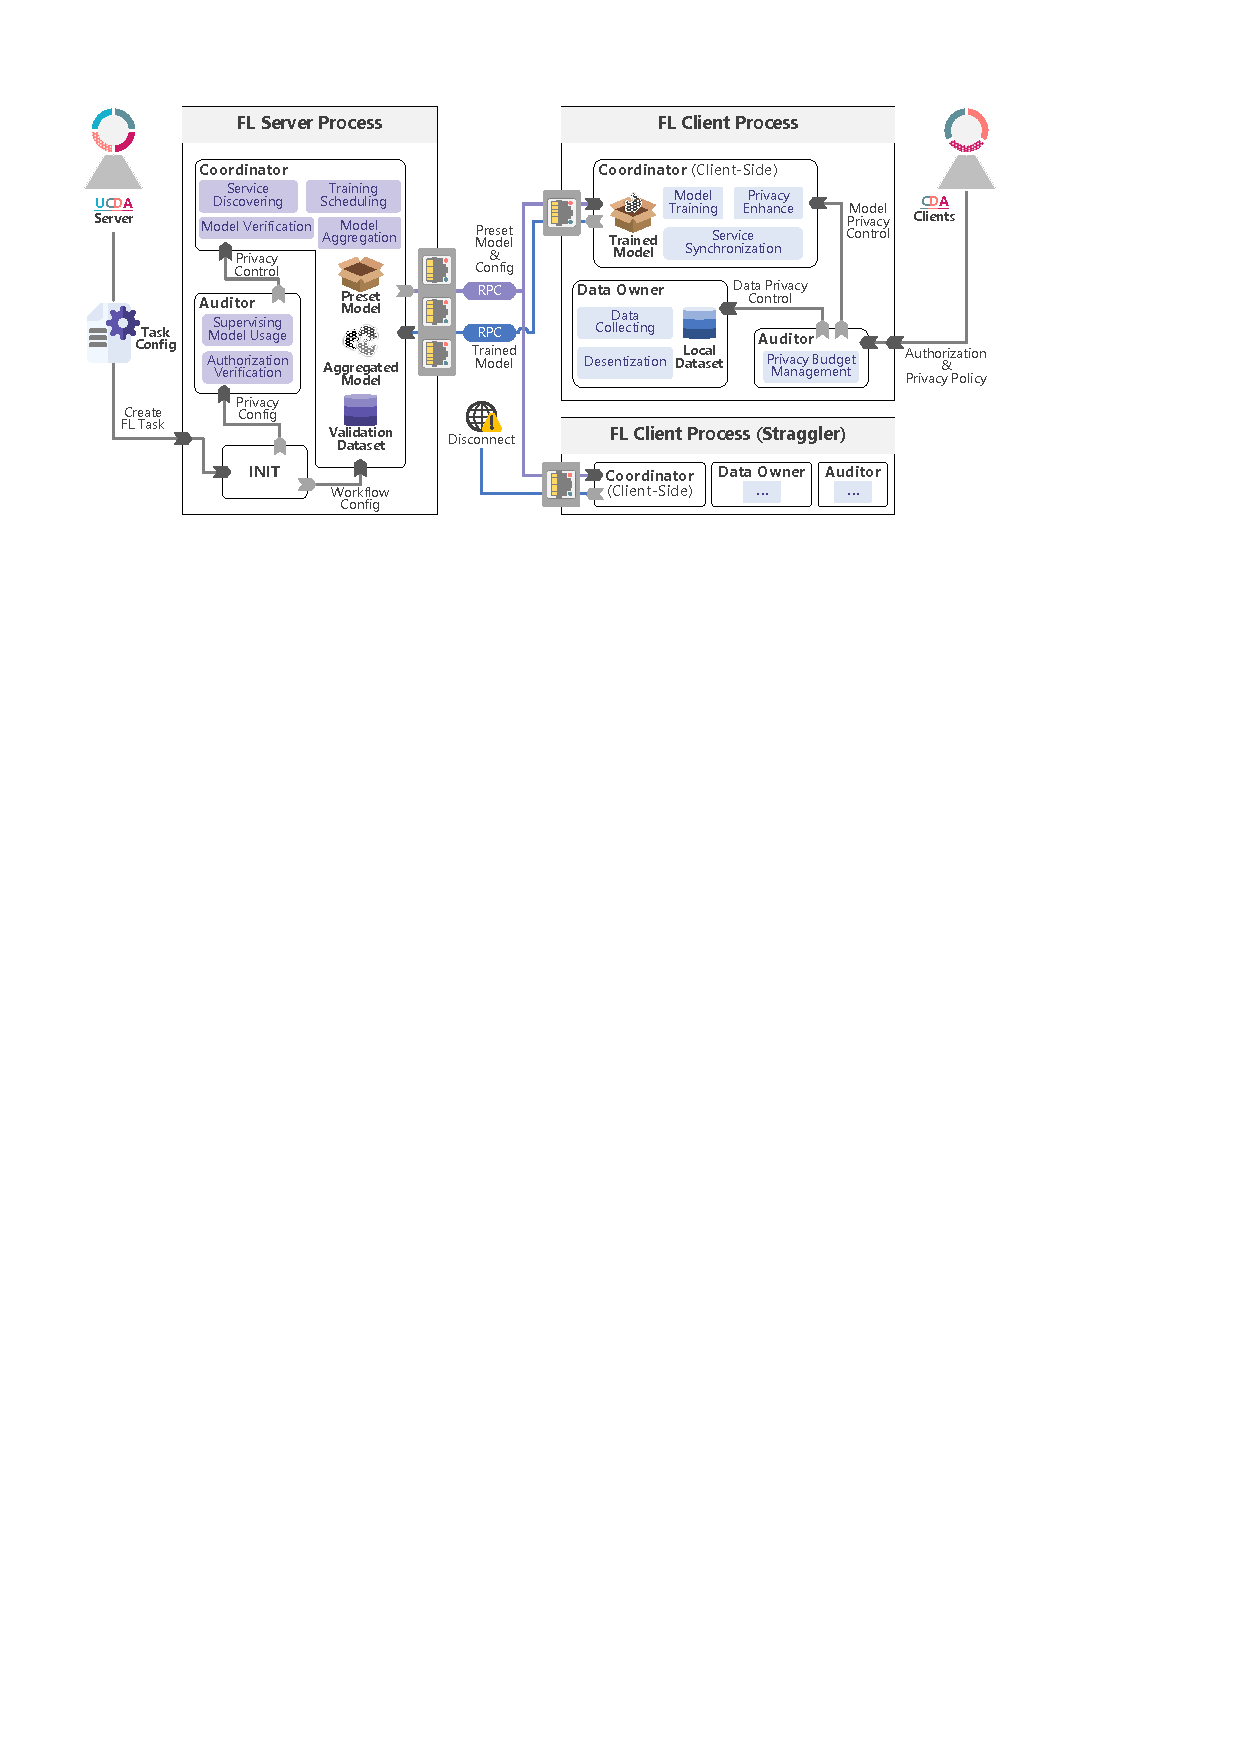
\includegraphics[width=\linewidth]{fig/fl_frame.pdf}
    \caption{An overview of traditional FL systems. (U: model User, C: Coordinator, D: Data owner, A: Auditor)}
    \Description{}
    \label{fig:fl}
  \end{figure}

Fig.~\ref{fig:fl} illustrates the typical architecture of FL systems, which as a distributed modeling toolkits consists of server part and client part. 
In a general FL setting, the server part is the central aggregator installed in a trusted cloud environment, while the client part of software can operate in different operating environments on client devices. 
The server and clients are connected via Internet and typically with the help of Remote Procedure Call (RPC) interface for coordinating~\cite{zhang2022felicitas, abadi2016tensorflow, liu2021fate, beutel2020flower, he2020fedml, foley2022openfl}.
We use four colors to represent the four FL roles and the colors with grid lines indicate non-essential roles.
For example, in Fig.~\ref{fig:fl}, the UCDA server takes on the roles of model user, coordinator and audior in traditional FL. 
However, it is no necessary to hold training data or validation data, so the role of data owner is non-essential.
To illustrate the workflow of traditional FL, we leverage the vanilla FL framework Federated Averaging (FedAvg)~\cite{mcmahan2017communication, bonawitz2019towards} as an example.

First, the FL server pre-defines the objective modeling task and initializes the server process.
Secondly,  the coordinator in server-side specifies a preset global model and the operational parameters.
Thirdly, the coordinator discovers the availability of clients' FL services, boardcasts the global model and training config to them. The training config contains bath size, local epoch round, optimizer parameters and so on. Then, the coordinator will wait for the trained results contributed by the coordinator in clients-side and drop those clients with network problems.
Finally, the server aggregates the trained resultes received from various clients into the global model and begins a new round based on this aggregated global model. 
The aggregation strategy adopted in FedAvg is the weighted model parameters based on the size of local dataset, which means the global objective of FL can be regarded as a joint objective function of clients. 
By this way, the FL server can learn a generalized global model by jointly optimizing all local optimization objectives and incorporating the latent knowledge from the local models.
Although the auditor component was not included in earlier FedAvg, it play an important role in the later business-ready FL frameworks~\cite{liu2021fate,roth2022nvidia, ziller2021pysyft}.

However, in comparing FedAvg workflow described above with Fig.~\ref{fig:fl}, it is easy to notice that the client part has been excluded.
This is because we are elaborating from a server-side perspective, which is usual way FL is presented~\cite{mcmahan2017communication, li2020ditto, caldas2018leaf}.
Actually, the underlying reason is that in traditional FL, the client-side process is tightly coupled with server-side process, and there is no alternative for clients other than to either accept or reject the training scheduling from the server wholesale.
So the clients are not considered as an autonomous entities but rather work as subordinates to server.
In this server-domianted cooperation framework, the benefits and autonomy of clients are compromised, which hinders their enthusiasm to participate in FL network and subsequently limits the applicability of FL.
From this perspective, we summarize the limitations of traditional FL in the next section, which motivates us to explore more innovative sustainable FL cooperation frameworks.

\subsection{Limitations of Traditional FL}\label{sec:limitations_FL}
Previous surveys~\cite{kairouz2021advances, zhang2022federated, alazab2021federated, nguyen2021federated, zhu2022blockchain, li2020federated, yang2019federated, tan2022towards} has extensively discussed the challenges in FL systems from various aspects.
However, the cooperation mechanism of FL systems has been overlook because almost all mainsteam FL frameworks follow a same FL prototype~\cite{mcmahan2017communication}, which shape the form of current FL frameworks: a modeling software.
We summarize three inherent limitations of traditional FL cooperation mechanism: (1) \textbf{Server-client Coupling}, (2) \textbf{Low Model Reusability}, (3) \textbf{Non-public}.

\subsubsection{Server-client Coupling} 
% 设备异构 从客户端层面,从服务端层面
% 不合理假设,稳定的链接和已经安装好了软件(侵入式的,后台运行,损害客户端的独立性,恶意软件,资源浪费
The tightly-coupled server-client design is a major limitation of FL systems. From the perspective of FL service providers, adapting the programs to heterogeneous client hardware and software components, such as various operating and database systems, processor and storage architectures, communication protocols, energy constrains and data licenses, is a challenging task that significantly increases the complexity of the FL systems. 
    
On the other hand, the invasive software deploy mode compromises the integrity of client environments and expose them to new privacy risks.
Specifically, the coordinator components (client-side) pushed by the server may not offer demanded privacy control mechanisms~\cite{zeng2021fedlab, caldas2018leaf, mcmahan2017communication}, or cause resource depletion on client-side~\cite{bonawitz2019towards, niu2020billion, chen2020deep}, or even piggyback malicious executable codes~\cite{li2017understanding}.
So the auditor role of client is non-essential as depicted in Fig.~\ref{fig:fl}, not only because the client maybe lacks a corresponding policy for FL training, but also because its privacy is not completely under its control.
Likewise, the malicious clients can also exploit the vulnerability in the aggreagation strategy to currupt the FL tranining process~\cite{bouacida2021vulnerabilities, sattler2020byzantine, park2021sageflow, fang2020local} or insert backdoors~\cite{bagdasaryan2020backdoor, wang2020attack}.
In addition, the unstable network environment can drive clients to drop out from traning (i.e. straggler effect), thereby reducing system efficiency~\cite{reisizadeh2019robust, park2021sageflow}.
Therefore, the server-client coupling design of traditional FL systems make them susceptible to unpredictable runtime environments, leading to system vulnerability and low reliability.

\subsubsection{Low Model Reusability} % 模型的移植性 不可持续 模型的可发现性
The traditional FL scheduling follows a task-centric manner and terminates once the training reaches a preset number of rounds or meets traget metrics on global model set by FL server~\cite{bonawitz2019towards}.
As a result, only FL server can guarantee having the latest global model after the task is terminated.
This ad-hoc modeling paradigm results in low model reusability and transportability.
For example, if a client who participated in the previous training turn wants to continue training, they can only start the task from scratch unless they have the up-to-date global model.
Meanwhile, since only FL server is able to maintain the complete modeling trajectory, it is difficult for the client to roll back the training itself to eliminate the potential privacy risk.
Furthermore, the non-deliverable scheduling mechanism of FL tasks also hinders inter-task model reuse, which leads to unnecessary wasted energy and time on participants that have been involved in similar tasks.

\subsubsection{Non-public} % 无法自由发起任务,不提供公共接口
As we mention in Section~\ref{sec:flsystems}, except PySyft~\cite{ziller2021pysyft}, the application scenarios of mainstream FL frameworks~\cite{liu2021fate, abadi2016tensorflow, zeng2021fedlab, caldas2018leaf, ibmfl2020ibm, he2020fedml, beutel2020flower, roth2022nvidia} aim to provide private collaborative ML traning service, and there is no any accessible FL platform for the public.
Although there have been real-world deployment practices of FL for the public with scales of millions~\cite{bonawitz2019towards} and billions~\cite{niu2020billion}, these have been carried out only by tech giants with a massive base of active users. For an individual user, there is no practical way to organize such a large-scale FL training network.

But in fact, due to the limitations in the cooperation mechanism mentioned above, data owners are not sufficiently motivated to participate in this server-take-all FL training network even if it is public accessible. Therefore, the cornerstone of buliding a sustainable open FL platform is to create a reciprocal FL cooperation framework, followed by corresponding multi-source knowledge aggregation strategies, which we discuss in the following sections.

\section{Query-based Federated Learning}
\label{sec:query}
\subsection{Overview}
\label{sec:query_overview}
Let us continue by establishing a sustainable open FL platform based on a query-based cooperation framework.
An overview of this platform is presented in Fig.~\ref{fig:query}, the desin philosophy behind this framework is to break the coupling between FL server and clients.
In the query-based FL systems, all traditional FL roles and components are maintained on an open model repository called Model Community. The Model Community privdes a one-stop ML models redistribution and reuse service, including model indexing, automatic batch model reuse, license management, privacy control and so on.
In addition to large-scale pretrained models like BERT~\cite{devlin2018bert}, BLOOM~\cite{scao2022bloom} with great generalization abilities, we also encourage individuals to upload their task-specific models trained on limited domain data to boost the knowledge mining within models, aka model mining~\cite{you2021workshop}.
The derivatives of model mining can learn representations from multiple domains, resulting in more promising performance that can be evaluated by platform users.
Furthermore, the contributors can release models under applicable licenses, granting them distribution control and legal protection of their intellectual property (IP).
In summary, the properties of query-based FL are:
(1) \textbf{Model Agnostic}, as there are no restrictions on the types and architectures of the models uploaded by users;
(2) \textbf{Contactless}, as communication channels need not be maintained; 
(3) \textbf{Community-powered}, whereby sharing models enrichs the entire community.

\begin{figure}[t]
  \centering
  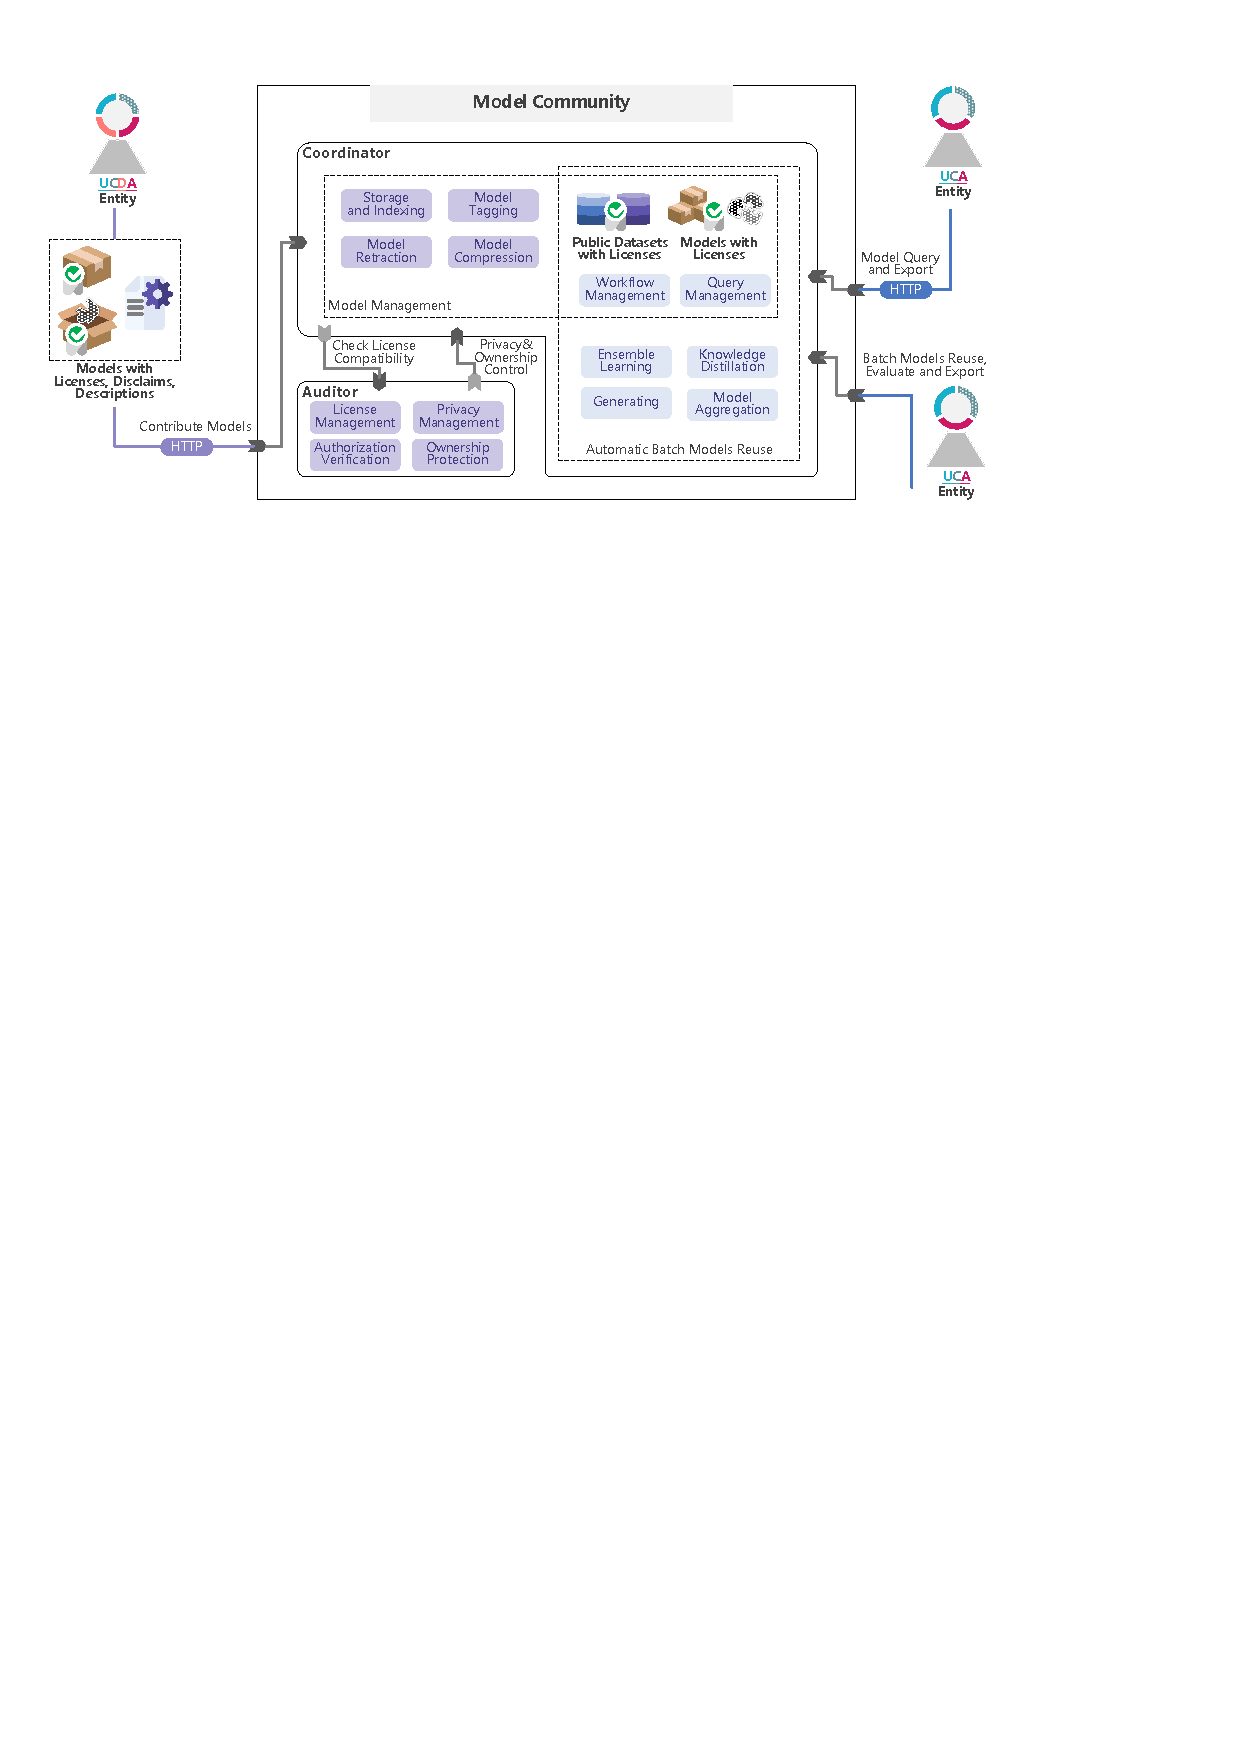
\includegraphics[width=\linewidth]{fig/query_frame.pdf}
  \caption{An overview of query-based FL systems. (U: model User, C: Coordinator, D: Data owner, A: Auditor)}
  \Description{}
  \label{fig:query}
\end{figure}

Actually, we aim to advocate a novel SaaS~\cite{brereton1999future} ML platform with automatic batch model reuse integrated, which has potential to leverage the transportability of models to address previously unexplored ML problems.
Due to the high computational demands of deep learning, current ML platforms primarily concentrate on computing, for example, MaaS, MLaaS, FLaaS provide ML models deployment and development services to handle user-specified tasks (ref. Section~\ref{sec:aas}).
On the other hand, there are several ML platforms provide open model search and download services. 
So, can we leverage leverage off-the-shelf open model platforms to build a query-based FL system?
Unfortunately, these platforms are designed solely for sharing and are no suitable for more advanced functionalities such as model ensemble~\cite{jacobs1991adaptive} and knowledge distillation~\cite{hinton2015distilling}, we will explain the reasons in the following section.

% Model Mining

\subsection{How to Query for Models}
\label{sec:how2query}
To establish a query-based FL platform, the first thing that comes to mind is how to query for models.
Unlike traditional ML model sharing repositories that mainly query for a specific model by name, it requires an efficiency approach to export a batch of target models that ready for ensemble or distillation.
We summaried the filter conditions of existing DNNs sharing repositories in Table.~\ref{table:repository}.
The prevailing method for querying models involves searching for the desired model by its name, datasets used, and the associated tasks.
To illustrate, one might search for the model name GPT~\cite{radford2019language}, models trained on the MNIST dataset~\cite{lecun2010mnist}, or models capable of performing image segmentation tasks.
However, this model retrieval method requires the users have a strong priori knowledge in data science, thus raising the barrier for knowledge mining within models.
For example, there is no effective way to acquire a batch of image classfication models that contains the knowledge of \textit{lesser panda} for further distillation.
A compromise solution is to manually search the schema of each dataset one-by-one and subsequently search for models trained on those datasets.

As shown in Table.~\ref{table:repository}, most DNNs repositories are simply list the description of input/output (e.g., NVIDIA NGC, OpenVINO) or even just present the source codes (e.g., Tensorflow Hub, Pytorch Hub).
This lack of unified convention for model input/output poses a challenge for query-based FL.
Additionally, most of DNNs repositories do not enable querying models by licenses, resulting in the cumbersome task of individually handling model licenses and ensuring compatibility among different licenses.
Hence, it is imperative to reconsider the design of DNNs repositories to enable quick identification of readily reusable models for knowledge aggregation. We further suggest following filter conditions for query-based FL.

\begin{table}[t]
  \caption{Filter conditions and characteristics of DNNs repositories. \checkmark : Supported, \ding{55} : Unsupported, \textbf{!} : Information provided but unsearchable, listed in descending order by number of released models.}
  \label{table:repository}
  \footnotesize
  \begin{tabular}{|l|c|c|c|c|c|c|c|c|}
  \hline
  & \multicolumn{1}{l|}{DS Name} & \multicolumn{1}{l|}{Model Architecture} & \multicolumn{1}{l|}{Modality/Task} & \multicolumn{1}{l|}{Tag} & \multicolumn{1}{l|}{License} & \multicolumn{1}{l|}{Input-Output} & \multicolumn{1}{l|}{Batch Export} & \multicolumn{1}{l|}{\# of Models}\\ \hline
  Hugging Face\tablefootnote{https://huggingface.co}
  & \checkmark & \checkmark & \checkmark & \checkmark & \checkmark & \textbf{!} & \ding{55} & 133,641 \\ \hline
  Model Zoo\tablefootnote{https://modelzoo.co/} & \checkmark & \checkmark & \checkmark & \checkmark & \ding{55} & \ding{55} & \ding{55} & 3,426 \\ \hline
  Tensorflow Hub\tablefootnote{https://tfhub.dev/}& \checkmark & \checkmark & \checkmark & \checkmark & \textbf{!} & \textbf{!} & \ding{55} & 1,356 \\ \hline
  NVIDIA NGC\tablefootnote{https://catalog.ngc.nvidia.com/models} & \textbf{!} & \checkmark & \checkmark & \checkmark & \textbf{!} & \textbf{!} & \ding{55} & 527 \\ \hline
  OpenVINO\tablefootnote{https://docs.openvino.ai/latest/model\_zoo.html} & \textbf{!} & \checkmark & \checkmark & \ding{55} & \textbf{!} & \textbf{!} & \checkmark & 278 \\ \hline
  Pytorch Hub\tablefootnote{https://pytorch.org/hub/} & \textbf{!} & \checkmark & \ding{55} & \ding{55} & \ding{55} & \textbf{!} & \ding{55} & 49 \\ \hline
  \end{tabular}
\end{table}

\subsubsection{Data Description} % 数据的domain和统计特征,数据的正确性,如何打标签,
Similar with the data heterogeous challenges in FL~\cite{liqb2022federated}. The local datasets of contributors have varing quality and contain intractable biases, imbalances and noisies that can be attributed to the natural characteristics of demographic or improper data collection mechanisms~\cite{dayan2021federated}.
Besides, label errors pervasive even in open datasets~\cite{northcutt2021pervasive}. 
So, in addition to searching for domain-specific datasets based on their data descriptions, we are also seeking such descriptions for the purpose of future traceability and debugging.
The data description can consist of statistical analysis results or the visualization diagrams that used to profile the data distribution~\cite{li2020multi} and complementary provenance information.

\subsubsection{Workflow and History}
\label{sec:workflow&history}
The process of building an ML model is iterative, involving repeated hyperparameter tuning and architecture exploration, resulting in abundant workflow and historical trajectory data.
This information includes pipelines, model structures, hyperparameter values for pre-training and fine-tuning, test metrics, and results. 
These data can be useful in filtering models that meet specific requirements, such as those with data standardization in preprocessing or evaluated using mean average precision (mAP).
Instead of manually saving and uploading the logs and configuration files, a more efficient method is to leverage ML workflow management tools~\cite{vartak2016modeldb}, such as MLflow~\footnote{https://mlflow.org} and Neptune~\footnote{https://neptune.ai}, to automatically track and store the ML workflow during model building process. 
This information can also assist in identifying potential model plagiarism within the model community.
In addition, to ensure that the computational consumption of models is within budget, Deep Learning Profiler~\footnote{https://docs.nvidia.com/deeplearning/frameworks/dlprof-user-guide/index.html} can be leveraged to generate a report that displays the FLOPS and bandwidth requirements.

\subsubsection{Software Dependency}
ML models are software that depend on underlying ML libraries, so it is important to declare the dependencies of the model to analyze software compatibility between batches of models. 
For instance, resource-constrained devices may need to trim down the list of software-dependent libraries to meet limited storage space requirements~\cite{david2021tensorflow}.
In some cases, contributed models may rely on other models as dependencies. 
For example, Fast R-CNN~\cite{girshick2015fast} uses VGG16~\cite{simonyan2014very} as its backbone. 
It is crucial to release this information for further model license compatibility analysis.

The aforementioned filter conditions provide comprehensive coverage of the ML modeling process. 
However, there are additional requirements depending on the reuse mechanisms of the model retrieval side. 
For example, FedAvg~\cite{mcmahan2017communication} aggregates the local models weights element-wise, which requires full access to the models. 
In contrast, MoE with a gating network~\cite{jacobs1991adaptive} only ensembles a batch of model outputs, so the individual models can remain blackboxes in this scenario.
So, in the context of software licenses or model licenses, the batch models reused by FedAvg should be released as source code, while those reused by MoE can be released as binary executable modules (e.g. dynamic linking).
The above distinction is crucial for ensuring that model reuse results meet the legal framework, and this has been overlooked in traditional FL.
We will expand on this topic in the following section.

\subsection{How to Reuse Batch of Models}
\label{how2reuse}
Once we have acquired a certain number of models that can contribute to the new target task, the next step is to reuse the knowledge of these pre-trained models, i.e., transfer their knowledge from source domain to the target domain~\cite{pan2009survey}.
However, before deciding on how to reuse the model, it is important to ensure that the necessary legal rights and permissions have been obtained. 
This may involve reviewing the terms and conditions of the licenses under which the models were released or obtaining permission from the original creators or copyright holders.
Therefore, in this section, we will not focus on the technical details of how to reuse models, which is already covered by many related surveys, such as Transfer Learning~\cite{pan2009survey}, Ensemble Leanring~\cite{zhou2012ensemble}, Domain Adaptation~\cite{wang2018deep}, Knowledge Distillation~\cite{wang2021knowledge}, Deep Generative Models~\cite{cao2022survey} and Model Fusion~\cite{ji2021emerging}.
Meanwhile, the specific model reuse technique or techniques used is at the user's discretion, and the query-based FL platform we advocate is not bound or restricted to any particular model reuse algorithm.
Innovatively, we study how to reuse batch of models, from the perspective of \textbf{legal compliance}.
%Therefore, the focus of this section is how to reuse batch of models, from the perspective of legal compliance.

The machine learning community benefits from the openness of ideas and code, and many high-impact ML conferences and journals encourage authors to publish their source code and dataset to research platforms like Papers With Code~\footnote{https://paperswithcode.com} and Code Ocean~\footnote{https://codeocean.com} to increase exposure and facilitate reproducibility.
To restrict the use of ML techniques for unethical purposes (i.e. Deepfakes~\cite{mirsky2021creation}) and protect the IP of creators, models are typically published under a license agreed upon by the licensor.
Here, we summary the granted rights, restrictions and enforcements of licenses for ML models posted on Hugging Face in Table~\ref{tab:licenses}.
The following sections will provide a detailed survey of these licenses.


\begin{table}[t]
  \centering
  \scriptsize
  \caption{Licenses for ML models available on Hugging Face with a focus on their rights, restrictions and enforcements, grouped by free software licenses, AI model licenses, free content or database licenses in descending order of number of models (GPL, BSD, LGPL, CC licenses with unspecified versions are excluded, the similar revisions are merged). \checkmark : Permited or Required, \ding{55} : Not Permited or Not Required, \textbf{!} : Not Explicitly Permited, * : Copyleft License, $^{\dagger}$ : Public Domain License. Only the source code of the original work under AFL-3.0 or Artistic-2.0 is required to be disclosed. You may not distribute the modified materials licensed under CC-BY-NC-ND or CC-BY-ND.}
  \label{tab:licenses}
  \vspace{-3mm}
  \begin{tabular}{r||ccc|ccc|cccc|c|p{3.5cm}}
    \toprule
    Licenses
    & \multicolumn{1}{P{90}{2.0cm}}{Modify / Merge} &
      \multicolumn{1}{P{90}{2.0cm}}{Redistribution} &
      \multicolumn{1}{P{90}{2.0cm}}{Sublicensing} & 
      \multicolumn{1}{P{90}{2.0cm}}{Commercial Use} & 
      \multicolumn{1}{P{90}{2.0cm}}{Patent Use} & 
      \multicolumn{1}{P{90}{2.0cm}}{Trademark Use} &
      \multicolumn{1}{P{90}{2.0cm}}{State Changes} &
      \multicolumn{1}{P{90}{2.0cm}}{Disclose Source} &
      \multicolumn{1}{P{90}{2.0cm}}{Responsible-use Restrictions} &
      \multicolumn{1}{P{90}{2.3cm}}{License/Attribution Preservation} &
      \multicolumn{1}{P{90}{2.0cm}}{\# of Models} &
      \multicolumn{1}{c}{Licensed Materials / Remarks}    \\
    \midrule

    \rowcolor{green!15}
    Apache-2.0 & \checkmark & \checkmark & \checkmark & \checkmark & \checkmark & \ding{55} & \checkmark & \ding{55} & \ding{55} & \checkmark & 23,519 & BERT~\cite{devlin2018bert} \\

    MIT &  \checkmark & \checkmark & \checkmark & \checkmark & \textbf{!} & \textbf{!} & \ding{55} & \ding{55} & \ding{55} & \checkmark & 9,605 & GPT-2~\cite{radford2019language} \\

    \rowcolor{green!15}
    AFL-3.0 & \checkmark & \checkmark & \checkmark & \checkmark & \checkmark & \ding{55} & \checkmark & (\checkmark) & \ding{55} & \checkmark & 1,561 & Italian-Legal-BERT~\cite{licari2022italian} \\

    *GPL-3.0 & \checkmark & \checkmark & \ding{55} & \checkmark & \checkmark & \ding{55} & \checkmark & \checkmark & \ding{55} & \checkmark & 404 & CKIP BERT Chinese \\

    \rowcolor{green!15}
    Artistic-2.0 & \checkmark & \checkmark & \checkmark & \checkmark & \checkmark & \ding{55} & \checkmark & (\checkmark) & \ding{55} & \checkmark & 331 & Include original source \\

    BSD-3-Clause\&-Clear & \checkmark & \checkmark & \checkmark & \checkmark & \textbf{!} & \ding{55} & \ding{55} & \ding{55} & \ding{55} & \checkmark & 209 & CodeGen~\cite{nijkamp2022conversational}/ A MIT-style license \\

    \rowcolor{green!15}
    $^{\dagger}$WTFPL-2.0 & \checkmark & \checkmark & \textbf{!} & \checkmark & \textbf{!} & \textbf{!} & \ding{55} & \ding{55} & \ding{55} & \ding{55} & 131 & A MIT-style permissive license  \\

    *AGPL-3.0 & \checkmark & \checkmark & \ding{55} & \checkmark & \checkmark & \ding{55} & \checkmark & \checkmark & \ding{55} & \checkmark & 96 & Extended GPL covers SaaS  \\

    \rowcolor{green!15}
    $^{\dagger}$Unlicense & \checkmark & \checkmark & \textbf{!} & \checkmark & \textbf{!} & \textbf{!} & \ding{55} & \ding{55} & \ding{55} & \ding{55} & 90 & A MIT-style permissive license  \\
    %GPL & 1 & 2 & 3 & 4 & 5 & 6 & 7 & 8 & 9 & 10 & 63 &  \\

    BSL-1.0 & \checkmark & \checkmark & \checkmark & \checkmark & \textbf{!} & \textbf{!} & \ding{55} & \ding{55} & \ding{55} & \checkmark & 60 & A MIT-style permissive license \\
    %BSD & 1 & 2 & 3 & 4 & 5 & 6 & 7 & 8 & 9 & 10 & 43 &  \\

    \rowcolor{green!15}
    *GPL-2.0 & \checkmark & \checkmark & \ding{55} & \checkmark & \textbf{!} & \textbf{!} & \checkmark & \checkmark & \ding{55} & \checkmark & 34 & Not compatible with GPL-3.0  \\

    BSD-2-Clause & \checkmark & \checkmark & \checkmark & \checkmark & \textbf{!} & \textbf{!} & \ding{55} & \ding{55} & \ding{55} & \checkmark & 34 & A MIT-style permissive license  \\

    \rowcolor{green!15}
    *LGPL-2.1\&3.0 & \checkmark & \checkmark & \ding{55} & \checkmark & \checkmark & \textbf{!} & \checkmark & \checkmark & \ding{55} & \checkmark & 25 & For software libraries  \\

    *OSL-3.0 & \checkmark & \checkmark & \checkmark & \checkmark & \checkmark & \ding{55} & \checkmark & \checkmark & \ding{55} & \checkmark & 22 & Linking is not derivative work \\

    %BSD-3-Clause-Clear & 1 & 2 & 3 & 4 & 5 & 6 & 7 & 8 & 9 & 10 & 14 &  \\
    %LGPL & 1 & 2 & 3 & 4 & 5 & 6 & 7 & 8 & 9 & 10 & 12 &  \\
    \rowcolor{green!15}
    ECL-2.0 & \checkmark & \checkmark & \checkmark & \checkmark & \checkmark & \ding{55} & \checkmark & \ding{55} & \ding{55} & \checkmark & 12 & For education communities \\

    *MPL-2.0 & \checkmark & \checkmark & \checkmark & \checkmark & \checkmark & \ding{55} & \checkmark & \checkmark & \ding{55} & \checkmark & 9 & State changes under MPL only  \\

    \rowcolor{green!15}
    ISC & \checkmark & \checkmark & \textbf{!} & \checkmark & \textbf{!} & \textbf{!} & \ding{55} & \ding{55} & \ding{55} & \checkmark & 8 & MIT-style license w/o sublicense \\ % Permission to distribute this software for any purpose

    Zlib & \checkmark & \checkmark & \textbf{!} & \checkmark & \textbf{!} & \textbf{!} & \ding{55} & \ding{55} & \ding{55} & \checkmark & 8 & Rename if modified \\

    \rowcolor{green!15}
    *Ms-PL & \checkmark & \checkmark & \checkmark & \checkmark & \checkmark & \ding{55} & \ding{55} & \ding{55} & \ding{55} & \checkmark & 7 & Weak copyleft license \\ % Weak copyleft

    *EPL-1.0\&2.0 & \checkmark & \checkmark & \checkmark & \checkmark & \checkmark & \textbf{!} & \ding{55} & \checkmark & \ding{55} & \checkmark & 6 & Can link proprietary license code \\

    \rowcolor{green!15}
    NCSA & \checkmark & \checkmark & \checkmark & \checkmark & \textbf{!} & \ding{55} & \ding{55} & \ding{55} & \ding{55} & \checkmark & 4 & Include full text of license \\

    PostgreSQL & \checkmark & \checkmark & \textbf{!} & \checkmark & \textbf{!} & \textbf{!} & \ding{55} & \ding{55} & \ding{55} & \checkmark & 2 & A MIT-style license \\

    \rowcolor{green!15}
    OFL-1.1 & \checkmark & \checkmark & \ding{55} & \checkmark & \textbf{!} & \textbf{!} & \ding{55} & \ding{55} & \ding{55} & \checkmark & 2 & For font software \\

    %EPL-1.0 & 1 & 2 & 3 & 4 & 5 & 6 & 7 & 8 & 9 & 10 & 2 &  \\
    *EUPL-1.1 & \checkmark & \checkmark & \checkmark & \checkmark & \checkmark & \ding{55} & \checkmark & \checkmark & \ding{55} & \checkmark & 1 & License of EU covers SaaS \\
    %LGPL-2.1 & 1 & 2 & 3 & 4 & 5 & 6 & 7 & 8 & 9 & 10 & 1 &  \\

    \rowcolor{green!15}
    LPPL-1.3c & \checkmark & \checkmark & \checkmark & \checkmark & \textbf{!} & \ding{55} & \checkmark & \checkmark & \ding{55} & \checkmark & 1 & Covering  stewardship transfer \\
    
    \hline
    %\textbf{Model Licenses $\downarrow$} & \multicolumn{12}{l}{} \\
    \hline
    
    \rowcolor{yellow!15}
    CreativeML-OpenRAIL-M & \checkmark & \checkmark & \checkmark & \checkmark & \checkmark & \ding{55} & \checkmark & \ding{55} & \checkmark & \checkmark & 3,590 & Stable Diffusions v1~\cite{rombach2022high} \\

    OpenRAIL &  \multicolumn{10}{l|}{>Responsible AI License template, w/o full text} & 2,393 & ControlNet~\cite{zhang2023adding}  \\

    \rowcolor{yellow!15}
    BigScience-BLOOM-RAIL-1.0 & \checkmark & \checkmark & \checkmark & \checkmark & \checkmark & \ding{55} & \checkmark & \ding{55} & \checkmark & \checkmark & 196 & BLOOM~\cite{scao2022bloom} \\

    BigScience-OpenRAIL-M & \multicolumn{10}{l|}{>Same as BigScience-BLOOM-RAIL-1.0} & 155 & A general version of 1.0 \\
    
    \rowcolor{yellow!15}
    OpenRAIL++ & \multicolumn{10}{l|}{>Same as CreativeML-OpenRAIL-M} & 72 & Stable Diffusion v2~\cite{rombach2022high} \\

    OPT-175B & \checkmark & \ding{55} & \ding{55} & \ding{55} & \ding{55} & \ding{55} & \ding{55} & \ding{55} & \checkmark & \checkmark & $\approx66$ & OPT LLM~\cite{zhang2022opt} \\

    \rowcolor{yellow!15}
    SEER &  \multicolumn{10}{l|}{>Same as OPT-175B, ban on reverse-engineer} & / & SEER Vision Model~\cite{goyal2022vision} \\
    
    \hline
    \hline

    \rowcolor{blue!15}
    CC-BY-4.0\&3.0\&2.5\&2.0 & \checkmark & \checkmark & \ding{55} & \checkmark & \ding{55} & \ding{55} & \checkmark & \ding{55} & \ding{55} & \checkmark & 1,740 & RoBERTa-SQuAD2.0~\cite{rajpurkar2016squad} \\

    *CC-BY-SA-4.0\&3.0 &  \checkmark & \checkmark & \ding{55} & \checkmark & \ding{55} & \ding{55} & \checkmark & \checkmark & \ding{55} & \checkmark & 590 & LEGAL-BERT~\cite{chalkidis2020legal} \\

    \rowcolor{blue!15}
    *CC-BY-NC-SA-4.0\&3.0 & \checkmark & \checkmark & \ding{55} & \ding{55} & \ding{55} & \ding{55} & \checkmark & \checkmark & \ding{55} & \checkmark & 556 & LayoutLMv3~\cite{huang2022layoutlmv3} \\

    CC-BY-NC-4.0\&3.0\&2.0 & \checkmark & \checkmark & \ding{55} & \ding{55} & \ding{55} & \ding{55} & \checkmark & \ding{55} & \ding{55} & \checkmark & 499 & GALACTICA~\cite{taylor2022galactica} \\

    \rowcolor{blue!15}
    $^{\dagger}$CC0-1.0 & \checkmark & \checkmark & \textbf{!} & \checkmark & \ding{55} & \ding{55} & \ding{55} & \ding{55} & \ding{55} & \ding{55} & 165 & BlueBERT~\cite{peng2019transfer} \\

    CC-BY-NC-ND-4.0\&3.0 & (\checkmark) & \ding{55} & \ding{55} & \ding{55} & \ding{55} & \ding{55} & \ding{55} & \ding{55} & \ding{55} & \checkmark & 21 & NonCommercial, NoDerivatives \\

    \rowcolor{blue!15}
    $^{\dagger}$PDDL & \checkmark & \checkmark & \checkmark & \checkmark & \ding{55} & \ding{55} & \ding{55} & \ding{55} & \ding{55} & \ding{55} & 16 & Database-specific license \\

    C-UDA & \checkmark & \checkmark & \checkmark & \ding{55} & \textbf{!} & \textbf{!} & \ding{55} & \ding{55} & \checkmark & \checkmark & 13 & Data for computational use only \\

    \rowcolor{blue!15}
    *LGPL-LR & \checkmark & \checkmark & \ding{55} & \checkmark & \textbf{!} & \textbf{!} & \checkmark & \checkmark & \ding{55} & \checkmark & 12 & LGPL for linguistic resources \\ %如果仅仅发布embedding模型,那么属于“使用语言资源的作品”,如果包含了语言资源或者加密后的资源,那么属于“使用语言资源的衍生物”,包含在此license范围

    *GFDL &  \multicolumn{10}{l|}{>Same as GPL, a free document license} & 12 & txtai-wikipedia \\

    \rowcolor{blue!15}
    CC-BY-ND-4.0 & (\checkmark) & \ding{55} & \ding{55} & \checkmark & \ding{55} & \ding{55} & \checkmark & \ding{55} & \ding{55} & \checkmark & 11 & Disallow making derivatives \\
    
    ODC-By & \checkmark & \checkmark & \ding{55} & \checkmark & \ding{55} & \ding{55} & \ding{55} & \ding{55} & \ding{55} & \checkmark & 7 & Automatic relicensing \\
    %但是只对derivative dataset有定义,对于model来可能不适用

    \rowcolor{blue!15}
    *ODbL & \checkmark & \checkmark & \ding{55} & \checkmark & \ding{55} & \ding{55} & \checkmark & \checkmark & \ding{55} & \checkmark & 6 & Automatic relicensing \\
    \bottomrule
  \end{tabular}
\end{table}

\subsubsection{Model Licensing Forms}
\label{sec:licensing}
As shown in Table~\ref{tab:licenses}, ML models are licensed in three main forms: as software (e.g. Apache, MIT, GPL), as a model (e.g. OpenRAIL), and as content/database (e.g. CC BY, PDDL).
The reason for the mixed use of licenses is the ambiguity in the dependency relationship between the ML code, model, and data.
Thinking in terms of software, ML models can be released with reproducable code and be considered as a component of software.
So many open software licenses are naturally deferred for licensing of models.
The most popular license is Apache-2.0, which is a permissive open software license that allows the freedom to make derivative works.
However, the model building process also relies on a massive amount of data~\cite{lecun2015deep} that may be licensed under different licenses, which can lead to license conflicts.
A real-world example is BERT~\cite{devlin2018bert}, which was published under the Apache-2.0 license but pre-trained on English Wikipedia documents that are licensed under CC BY-SA 3.0.
This changing of license violates the requirement of the CC BY-SA 3.0, which states that any contribution must be distributed under the \textbf{same license} as the original work.

%We don’t claim ownership of the content you create with GPT-2, so it is yours to do with as you please. We only ask that you use GPT-2 responsibly and clearly indicate your content was created using GPT-2.

Thinking in terms of content and database, some word embedding models, such as GloVe~\cite{pennington2014glove}, compute vector representations of words based on licensed open linguistic resources.
These representations can be regarded as a translation of corpus and fall under the license of the original linguistic resources.
A more complex scenario arises when the model is fine-tuned with other data that has a different license, for example, fine-tune RoBERTa~\cite{liu2019roberta} (licensed under MIT) with SQuAD2~\cite{rajpurkar2016squad} (licensed under CC BY 4.0).
The resulting model can be interpreted as both derived works and combined works.

Not only limited to protecting the IP and controlling the diffusion of ideas, but AI companies and researchers are also concerned about licensees using their models for unethical purposes~\cite{jobin2019global, awad2018moral, yuste2017four}, which is usually not restricted by traditional licenses designed for software and content.
We can infer the concerns of unethical use of GPT-2~\cite{radford2019language} from its modified MIT license granted by its inventors, which states, \textit{We don't claim ownership of the content you create with GPT-2, so it is yours to do with as you please. We only ask that you use GPT-2 responsibly and clearly indicate your content was created using GPT-2.} 
However, such a statement lacks legal enforcement, and users may avoid accountability by convincing themselves that despite their efforts to minimize harm, they could not predict the AI artifact they generated would be used for harmful purposes.
On the other hand, the original licensing frameworks for software and content (e.g. MIT, CC BY) are not well suited to the data-driven ML. 
Many ML operations, such as training, fine-tuning, inference, and distillation, are not explicitly defined in traditional software and content licenses, leaving a potential legal loophole for licensees.

To address the unique challenges and considerations surrounding the use and distribution of ML models, several specific licenses for ML models have been proposed. 
CreativeML OpenRAIL-M license, proposed by Responsible AI~\cite{contractor2022behavioral}, is the most popular model-specific license on Hugging Face and enables legally enforceable responsible use.
By accepting this license, licensees must adhere to the use-based restrictions stated by the licensor, and these restrictions must also apply to derivative works.
With a multitude of different model licenses available, it becomes a challenging and tedious work to reuse them in bulk. 
It is therefore imperative to establish guidelines for selecting the licenses for models and other related components that are ready for query-based FL.


%The effect of copyleft-style behavioral-use clauses spreads the requirement from the original licensor on his/her wish and trust on the responsible use of the licensed artifact. This is why OpenRAILs require downstream adoption of the use-based restrictions by subsequent re-distribution and derivatives of the AI artifact, as a means to dissuade users of derivatives of the AI artifact from misusing the latter.

%OPT-175B/SEER LICENSE is not a copyleft license, as it does not require derivative works to be licensed under the same license or a compatible one. It is a proprietary license that allows users to use and reproduce the licensed models subject to certain restrictions.

\subsubsection{License Choosing Preferences}
\label{sec:choosing}
In query-based FL, the model community aims to promote the reuse of models contributed by users, which raises unique concerns about model licensing:
\begin{itemize}
  \item A model license ready for open FL paltforms should allow the \textbf{modification, combination and redistribution} of original works and any derived works; and
  \item \textbf{Sublicensing} right should be granted to lubricate the republication of derived works resulting from knowledge mining; note
  \item Some licenses enforce the source of the derived works to be \textbf{disclosed} and prohibit their \textbf{commercial use}, which hinders model selling~\cite{chen2019towards}; and
  \item Some licenses are \textbf{copyleft} (marked with * in Table.~\ref{tab:licenses}), which means the derivatives must be licensed under the same license or a compatible license, leading to potential license conflicts and proliferation~\cite{gomulkiewicz2009open}; last
  \item All granted rights are preferably \textbf{irrevocable} by the licensors~\cite{reddy2009jacobsen}.
\end{itemize}

Furthermore, it is important to consider the licensing of two other components when building and reusing models: data and algorithms, which may have entirely different license terms. 
Here, based on the comparisons between different licenses provided in Table~\ref{tab:licenses}, we present several strategies for selecting licenses in query-based FL to minimize conflicts.

\textbf{Preferences for Datasets or Databases}: CC0-1.0, PDDL, ODC-By > CC BY, C-UDA > LGPL-LR.
% 对于数据:训练:C-UDA 可以sublicense,但是不能商用。CC0 和 CC-BY 可用但是没明确sublicense,ODbL 自动license,但是copyleft,必须开源。对于finetune,除了上述数据外还可LGPL-LP
   
  Our recommended licenses for training datasets and databases for query-based FL are CC0-1.0, PDDL, ODC-By and CC BY (the preferred version of CC BY is 4.0 due to the grant of \textit{Sui Generis Database Rights in Art.1c}).
  CC0-1.0, PDDL and ODC-By are more permissive than CC BY since they do not require licensees to disclose any modifications made to the dataset or database. Additionally, CC0-1.0 and PDDL are public domain licenses and do not require the declaration of the original license.
  Although some of these licenses do not explicitly grant sublicensing rights, they provide an \textbf{automatic licensing} policy for downstream recipients.
  
  C-UDA is an alternative license that grants sublicensing rights, but it includes additional usage restrictions that limit its application to computational use only, which indicates commercial use of data is not allowed.
  Nonetheless, C-UDA explicitly exempts reused results from any restrictions, which is highly favorable for our scenario of model mining.
  To avoid license proliferation, it is not recommended to use any data under copyleft licenses for building models, as the resulted models could be seen as remixing and making derivatives of the original datasets, leading to potential conflicts between licenses.
  Among them, LGPL-LR is an exception because it contains an exemption clause for \textit{work that uses the Linguistic Resource (Art.3)}, which is suitable for end-to-end training, fine-tuning, and embedding. 
  But it is worth noting that the embedded representations may be considered \textit{translated straightforwardly into another language (Art.0)}, which falls within the scope of LGPL-LR license.
  
  An example of license proliferation is LEGAL-BERT~\cite{chalkidis2020legal}, which was trained on data from the Case Law Access Project~\footnote{https://case.law} (licensed under CC BY-SA 4.0). This restricts LEGAL-BERT to the same license and prevents further model reusing on datasets or models licensed under incompatible copyleft licenses, such as LGPL-LR and GPL.

  \textbf{Preferences for Software}: Apache-2.0, AFL-3.0, Artistic-2.0, ECL-2.0 > MIT, BSD-3-Clause\&-Clear, BSL-1.0, BSD-2-Clause, NCSA $\approx$ Ms-PL > WTFPL-2.0, Unlicense, ISC, Zlib, PostgreSQL.
  % 必须: sublicense, permissive. 
  % Rank1: Permissive Licenses with Patent right (But State Change)
  % Rank2: Not Explicitly Permited Patent or Trademark (No need State Change), Ms-PL weak permissive, 对object无需求, code需要为Ms-PL license
  % Rank3: 非常自由的协议,但是没有明确grant sublicense
  
  Our top recommended software licenses for training and reusing models are Apache, AFL, Artistic, and ECL.
  These permissive licenses allow modification and sublicensing, explicitly grant the use of patents and permit commercial use, and do not require the disclosure of the source code but only the stating of any changes made to the original work.

  The next set of recommendations are MIT, BSD, BSL, and NCSA. 
  These licenses do not explicitly grant patent rights but instead, do not require the stating of modifications made to the original work, thus avoiding the tedious task of tracking model reusing or incremental training procedures. 
  Ms-PL offers two advantages simultaneously, but it is a \textbf{weak copyleft} license that requires the modified source code to also be licensed under Ms-PL, and the derivative object code to be compliant with a license compatible with Ms-PL.
  Note that open software licenses do not provide a clear definition for software-generated outputs such as models. 
  It is unclear whether models are considered a portion of the software, and whether they are in source code form or object code form. 
  This ambiguity makes it difficult to determine the applicable clauses for models.
  
  Our latest recommended licenses include WTFPL, Unlicense, ISC, Zlib, and PostgreSQL.
  These licenses are very permissive and allow almost anything without restrictions.
  However, on the other side, these licenses also do not explicitly grant sublicensing rights and patent, which can lead to ambiguity in interpreting the license clauses.
  For the avoidance of doubt, copyleft licenses such as GPL, AGPL, LGPL, OSL, MPL, EPL, and EUPL are not recommended, despite the loophole that they do not have a specific definition for ML models.
  Although some of those copyleft licenses can be made compliant with others, we recommend isolating the software licenses from the resulting models to preserve the freedom to use the models further (e.g. close-source, relicense).
  
  \textbf{Preferences for Models}: Apache-2.0, AFL-3.0, Artistic-2.0, ECL-2.0 > OpenRAIL and its derivatives
  % The crux of the issue is really about control over the outputs.
  
  There are two recommended choices for model licenses for query-based FL. 
  The first is permissive open software licenses like Apache, AFL, Artistic, and ECL. 
  The second is open model-specific licenses like OpenRAIL and its derivatives.
  As shown in Table~\ref{tab:licenses}, the main difference between the two choices is that OpenRAIL offers additional user behavioral restriction clauses and enforces these restrictions via a copyleft-style agreement.
  For example, CreativeML OpenRAIL-M license claims \textit{Therefore You cannot use the Model and the Derivatives of the Model for the specified restricted uses ... You shall require all of Your users who use the Model or a Derivative of the Model to comply with the terms of this paragraph}.
  The restricted uses include actions that could cause harm, provide medical advice, generate or disseminate verifiably false information, and more.
  So, the model owners may adopt these licenses for the purpose of responsible model use.

  However, in practice, such discrimination of user behavior cannot completely guarantee that the models will not be misused, and may potentially compromise the openness of the models~\cite{perens1999open, greenbaum2016the}.
  The user behavioral restrictions stated in licenses can be compared to manufacturers prohibiting the use of their laptops for hacking, and furthermore, the vendors can be held jointly and severally liable for any future violations, which is unreasonable.
  Therefore,  including such statements in licenses may ultimately lead to the licensed materials becoming closed source. 
  Additionally, to enable remote control for the responsible use of AI, CreativeML OpenRAIL-M includes the clause \textit{You shall undertake reasonable efforts to use the latest version of the Model}, which requires licensees to keep up with the updates of the original work and may render their prior development efforts useless.
  Therefore, traditional permissive licenses, which follow worse-is-better design philosophy~\cite{gabriel1991rise}, are good choices for model licensing in query-based FL, as they promote openness and facilitate the sharing of publicly contributed models.

  The remaining model licenses, OPT-175B and SEER, are proprietary licenses that allow licensees to use and reproduce the licensed models subject to certain restrictions. 
  Given that their granted rights are revocable, we do not recommend using any content of works and derivatives under these licenses in query-based FL.

It is worth noting that the above discussion only deals with the licenses of inputs for open FL platforms, which aim to provide legal compliance and freedom of outputs as much as possible, but does not involve the copyright issue for the outputs.
In fact, except for some public domain dedication licenses like CC0-1.0, PDDL, Unlicense, and WTFPL, most licenses only grant non-exclusive rights for use and distribution, and the original copyright and attribution are retained by the licensors.
Whether the reused models are copyrightable is crucial for incentivizing model sharing and mining, so we will elaborate on this topic in the next section.

\subsubsection{Copyright of Reused Models}
\label{sec:generated content}
Software and computer code are indisputably copyrightable, but what about computer-generated content such as distillation and ensembles of models?
The copyrightable of a computer-generated work is controversial, which may depend on such as the level of creativity and originality and \textit{presence of at least minimal human creative effort at the time the work is produced}~\cite{national1979final}.
According to this definition, programmers who engage in model design and training meet the threshold requirements of copyrightability and own the copyright of the model. 
That is why all the licenses listed in Table~\ref{tab:licenses} contain claims of copyright.
But the debating point is whether the reused models also copyrightable?
Unfortunately, there is no universal answer to this question as it can depend on the specific case and fact pattern.
The crux is whether the efforts involved in reusing the model meet the minimum creative requirements for copyrightability.
For example, if we simply stack two models end-to-end, it may not meet the threshold for copyrightability. 
However, if we improve a basis model using distilled knowledge from other domains, that would be more likely to meet the requirements for copyrightability.
Except for copyrightability, the authorship of a reused model is also open to controversy, as it depends on whose \textit{original intellectual conceptions} the work embodies, and joint authorship is also possible~\cite{hedrick2019ithink}.

The determination of copyrightability and authorship of computer-generated content is an open issue that needs to be addressed through corresponding legislation~\cite{national1979final, hedrick2019ithink, margoni2018artificial}.
European Parliament regarded that \textit{consideration must first be given to assessing patent law in the light of the development of AI}~\footnote{https://www.europarl.europa.eu/doceo/document/A-9-2020-0176\_EN.html}.
The possible answers to the question of authorship of computer-generated models are model authors, model users, data owners, any combination of them, or no one~\cite{hedrick2019ithink}.
Licensors can also make efforts to clarify this issue by including relevant claims in their licenses.
For example, the license of Stable Diffusion~\cite{rombach2022high} explicitly states that \textit{Licensor claims no rights in the Output You generate using the Model}. 
Similarly, ChatGPT~\footnote{https://openai.com/blog/chatgpt}, even though it is a proprietary software of OpenAI company, its sharing \& publication policy~\footnote{https://openai.com/policies/sharing-publication-policy} states \textit{The published content is attributed to your name or company}.
Therefore, we are free to use their generated content for model reusing and can claim the copyright of reused models.
On the contrary, the licenses of OPT~\cite{zhang2022opt} and SEER~\cite{goyal2022vision} do not grant any copyright for the data produced by the licensed software. 
Given that, we should avoid using their derivatives and generated content in query-based FL to prevent copyright infringement.
Once we obtain the right to relicense the modification models, the choice of a new license depends on the application scenario of models. 
We further provide a flowchart in Fig.~\ref{fig:flowchart}(a) to guide the license selection in the context of model query and model reusing.

For now, we have provided a comprehensive perspective and suggestions regarding the regulations and legal issues related to batch model reusing with only one piece missing: the definition of terms and corresponding clauses for different reusing mechanisms in different licenses.
The terms definition for model reusing in different licenses is a novel and interesting issue that is rarely discussed. 
For example, interpreting model reusing as creating derivatives or combinations would involve different clauses in the licenses.
To provide a better understanding of these implications, let's first provide an overview of typical model reuse mechanisms.

\subsubsection{Batch Model Reuse Mechanisms}
\label{sec:taxonomy}
Instead of summarizing the batch model reuse mechanisms from a technological and algorithmic aspect, we propose grouping these mechanisms based on the classification of their resulting outputs for ease of justifying license clauses.
As shown in Fig.~\ref{fig:flowchart}(b), there are four categories of batch model reuse mechanisms: \textbf{Combination, Amalgamation, Distillation, and Generation}, each resulting in different forms of outputs and may correspond to different regulations in licenses.

\begin{figure}[t]
    \centering
    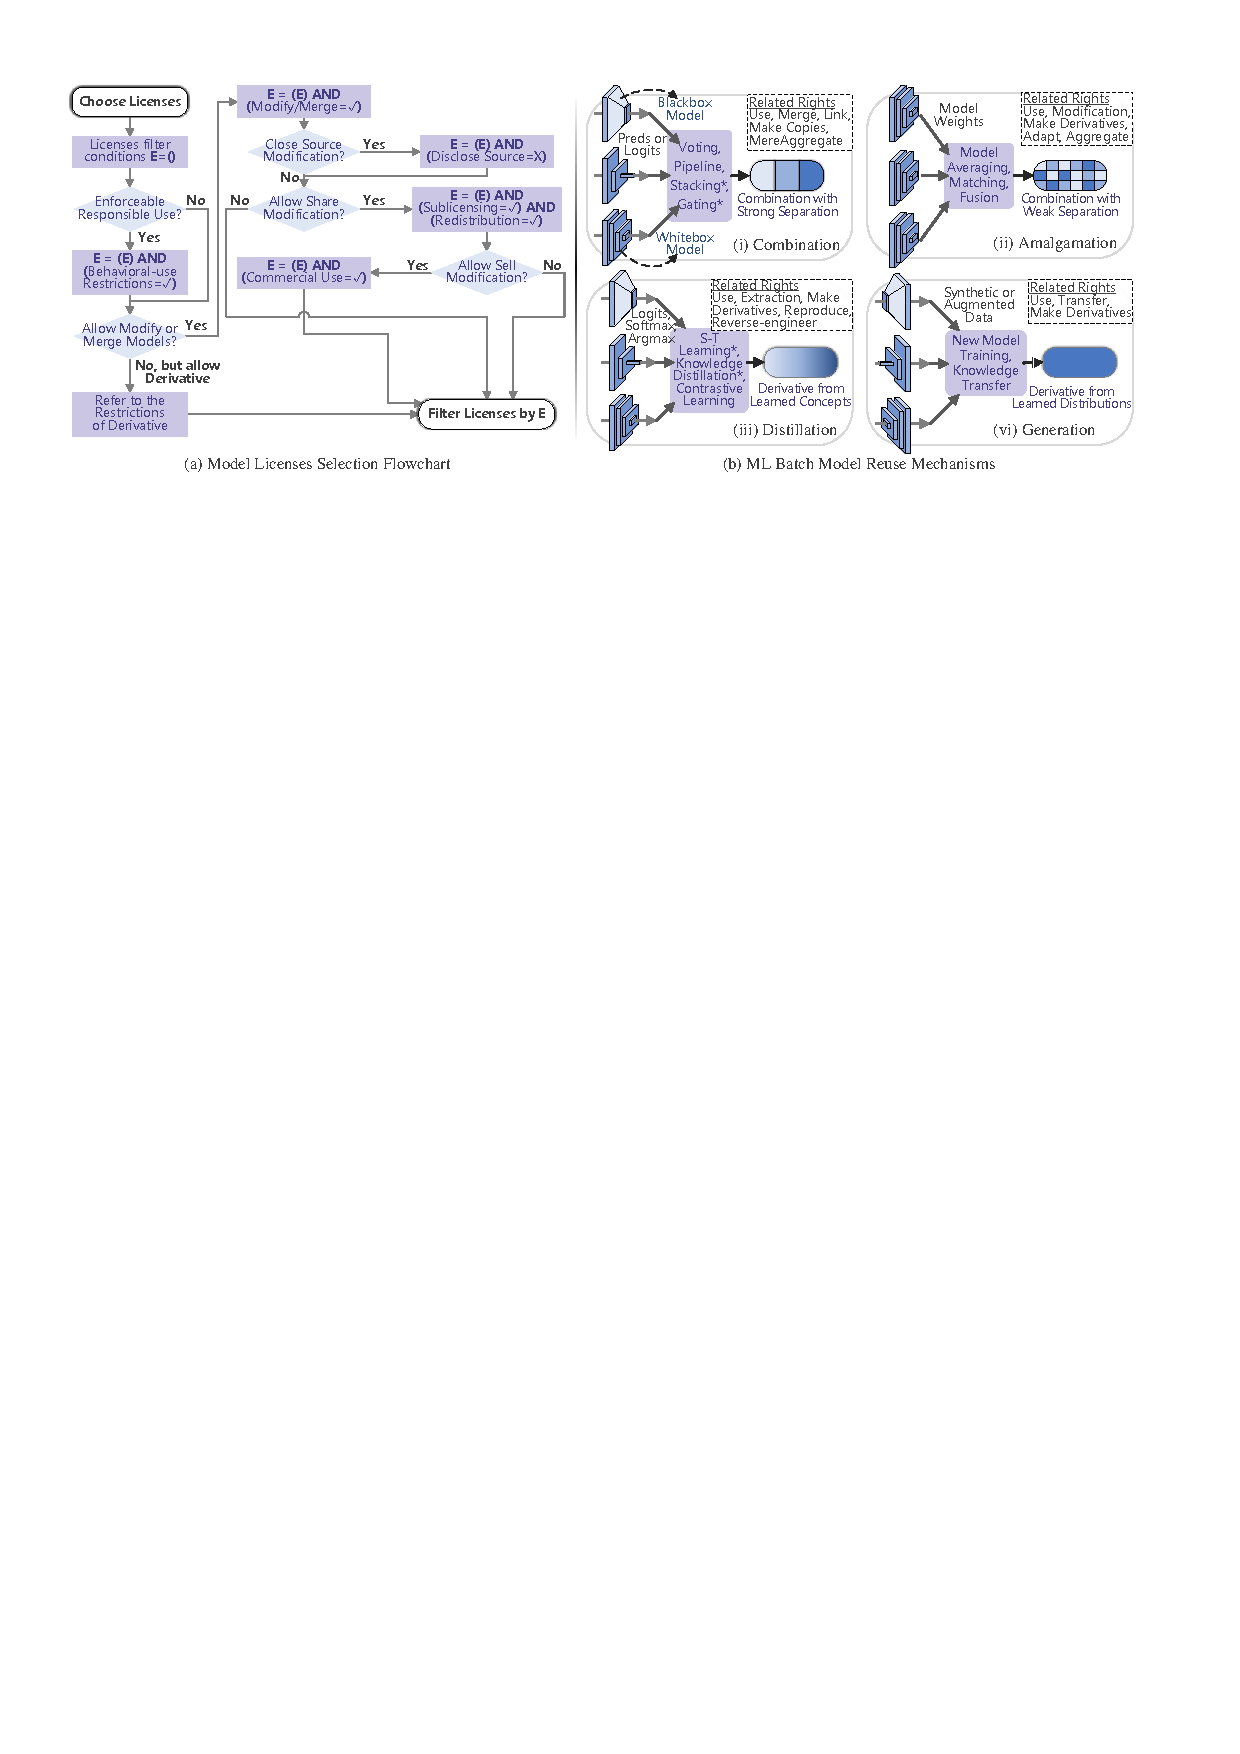
\includegraphics[width=\linewidth]{fig/flowchart.pdf}
    \caption{(a) Flowchart for model licenses selection in the context of model query and model reusing. (b) Proposed taxonomy categorizing batch model reuse mechanisms based on the reused results.}
    \Description{}
    \label{fig:flowchart}
\end{figure}

\textbf{Combination}~\cite{zhou2012ensemble} is a straightforward way to reuse batch of models (aka base learners), in which multiple models jointly contribute to the output by combination strategies such as averaging, voting, learning~\cite{jacobs1991adaptive, wolpert1992stacked}.
For regression estimates, averaging can improve the generalization by taking the mean of the outputs of all weak learners in a population. Additionally, the outputs of each learner can be weighted by extra parameters~\cite{perrone1995networks}, which can be determined by stacking estimators~\cite{wolpert1992stacked}, Bayes approach~\cite{clarke2003comparing} or backpropagation of gating networks~\cite{jacobs1991adaptive}. 
% Bayesian Model Averaging (BMA) -> Stacking with probabilities
Voting is a workaround strategy for classification tasks and also applicable for stacking and gating.
Both stacking and gating rely on an additional holdout or validation dataset for calculating extra parameters, marked as * in Fig.~\ref{fig:flowchart}(b). 
The difference is that gating can adapt the weights of each model's estimation based on the inputs, providing better generalizability performance of the combined model.

There are many \textbf{advantages} of combination mechanisms from the perspective of FL.
First, the input spaces of base models can be unaligned, which is ideal for the scenario of vertical FL~\cite{wu2022practical} where each client may have inconsistent features in their data.
Secondly, especially for query-based FL, it can simultaneously support multiple types and heterogeneous models, which means that it does not rely on any prior assumptions of the models, such as whether they are DNNs or decision trees, released with raw weights (whitebox) or binary forms (blackbox).
Thirdly, the tasks of models can be different if we pipeline the base models end-to-end, which is usually overlooked as a combination mechanism of models. 
Pipelining can fully leverage the transferability of models to solve previously unexplored ML problems.
% 举例说明 pipeline
For instance, Gao \textit{et al.}~\cite{gao2022precise} proposed a zero-shot dense retrieval system named HyDE by pipelining a natural language generation (NLG) model~\cite{ouyang2022training} and a natural language understanding (NLU) model~\cite{izacard2021towards}.
The generated content, which may lack factual grounding, from the NLG model is used as query embeddings to facilitate real document retrieval by the NLU model.
Similarly, through query-based FL, we can query a vicarious NLG model for a novel scenario, such as ProGen~\cite{madani2023large} for protein sequences generation, and quickly adapt this system to proteomics.
Not limited to that, we can query a batch of NLG models by a well-chosen filter condition and then combine models through averaging or gating to significantly expand the exploration space for knowledge discovery.
Lastly, the combinated models have strong separation from each other, meaning that we can add or remove a batch of models without significant changes to the remaining ones.
Meanwhile, combination mechanisms do not rely on the transparency of models and support blackbox sharing. 
Thus, the base model can establish loose connections with other models only through run scripts, providing revocability of such combination and circumvention of the restrictions of licenses.

On the other hand, instead of being treated as a challenge for FL~\cite{ma2022state}, the statistical heterogeneity and model heterogeneity nature of these crowdsourced models can actually enrich population diversity, which is crucial for creating a good ensemble~\cite{maclin1995combining, opitz1995generating}. 
\textbf{However}, the storage consumption of combined models increases linearly with the number of base learners, which can strain the communication resources of a collaborative model training network. 
As a result, alternative approaches involve amalgamating or merging multiple models to create a new consensus model. 
In the following, we provide a summary of these methods.

\textbf{Amalgamation} involves combining models through model parameters granularity operations, such as median~\cite{blanchard2017machine, pillutla2022robust} and coordinate-wise averaging with consideration of heterogeneity~\cite{mcmahan2017communication, li2018federated}, security~\cite{sun2019can}, scalability~\cite{reisizadeh2020fedpaq}, matching~\cite{wang2020federated, yu2021fed2}, specificality~\cite{gudur2020resource}, generalizability~\cite{qu2022generalized}, resulting in a combination with weak separation.
This reusing approach is widely used in FL works and is often referred to as "aggregation" procedures for local models.
%Here, we avoid using the term "aggregation" to distinguish it from "combination" given the latter is often used interchangeably with "combination" in software licenses (e.g. Artistic, GPL).
However, in order to avoid confusion with the term "combination," which is frequently used interchangeably with "aggregation" in software licenses (e.g., Artistic, GPL), we opt to use the term "amalgamation" instead.

FedAvg~\cite{mcmahan2017communication} is the most popular model averaging method in FL with many follow-up works. 
For instance, Sun \textit{et al.}~\cite{sun2019can} proposed applying norm thresholding of local model updates to defend against backdoor attacks.
Similarly, Blanchard \textit{et al.}~\cite{blanchard2017machine} proposed using more robust median-based amalgamation for resilience against Byzantine behavior.
Consider the ordering of parameters, Wang \textit{et al.}~\cite{wang2020federated} match and average the NNs parameters layer-wise across clients, based on their similarities.
Yu \textit{et al.}~\cite{yu2021fed2} further attribute the misalignment in FL models to the non-IID training data, propose allocating an independent structure for each class and updating models through a feature paired averaging strategy.
\textbf{Even though} amalgamation mechanisms can achieve a balance between model performance and resource efficiency by maintaining only one global model, they often rely on multiple rounds of communication to converge, which is not applicable in a query-based FL scenario.
Therefore, instead of trying to directly concatenate multiple sources of models while dealing with intricate parameter mismatch, transferring the latent knowledge learned by local models to a new model is a good alternative (i.e. Federated Distillation~\cite{jeong2018communication, jin2023feddyn}).

Another direction of model amalgamation is leveraging Bayesian nonparametrics to learn the shared global latent structures among local models~\cite{yurochkin2019bayesian, yurochkin2019statistical, lam2021model}. 
These methods, known as Model Fusion, can identify distributions of neural components across local models and only fuse the components with the same distribution, which can be regarded as a model compression between FedAvg (coordinate-wise averaging) and combination (w/o averaging).
However, the model fusion strategies rely on multiple communication rounds to boost the fusion efficiency, and the model performance of one-shot fusion is even worse than that of Ensemble.
Most recently, Su \textit{et al.}~\cite{su2023one}, inspired by null-space in continual learning~\cite{wang2021training, kong2022balancing}, propose MA-Echo which leverages layer-wise projection matrices to preserve the original loss of local models after amalgamation.
Their evaluation results present a moderate improvement in one-shot setting compared to FedAvg and ensemble.
\textbf{Unfortunately}, this improvement is not consistently observed in multiple-round experiments.
Meanwhile, to tackle the issue of catastrophic forgetting, FedPR~\cite{feng2023learning} follows similar ideas to facilitate the server's learning of visual prompts from clients for MRI reconstruction applications, \textbf{but} the improvement compared to FedAvg is limited even in multi-round setting.

It is worth noting that our taxonomy is based on the form of the resulting model, which may not be entirely consistent with the terminology used in the technical perspective.
For example, Bayes Model Averaging (BMA)~\cite{clarke2003comparing} estimates posterior probabilities of each model given the observed data, which results in a separable weighted model. 
Therefore, it should be classified as Combination instead of Amalgamation like FedAvg.
This novel taxonomy method is useful for analyzing compatibility with licenses. 
For example, the coordinate-wise operations or the fusion of model parameters generate fine-grained combinations of models that are almost irreversible, which corresponds to clauses such as adapt, modify, dynamic link, etc., in software licenses.

\begin{table}[t]
  \centering
  \footnotesize
  \caption{Summary of privacy-preserving \textbf{Distillation} works in the field of FL. Some works are listed multiple times because they contain multiple KD procedures with different strategies. Works with naming conflicts are distinguished by subscript.}
  \label{tab:distillation}
  \begin{tabular}{|ll|p{10cm}|}
    \hline
    \multicolumn{2}{|l|}{Strategies} & FL Studies \\ \hline
    \multicolumn{1}{|l|}{\multirow{2}{*}{KD@Server}} & w/ Validation Set & FedED~\cite{sui2020feded} \\ \cline{2-3} 
    \multicolumn{1}{|l|}{} & w/ Unlabeled Data & FedDF~\cite{lin2020ensemble}, One-shot FL~\cite{guha2018one}, FedBE~\cite{chen2020fedbe}, PerAda~\cite{xie2023perada}, FedET~\cite{cho2022heterogeneous} \\ \hline
    \multicolumn{1}{|p{1.6cm}|}{\multirow{5}{*}{\shortstack{KD@Client \\ w/ Local Data}}} & from Global Model & FedFusion~\cite{yao2019towards}, FedKD\textsubscript{2}~\cite{wu2022communication}, MOON~\cite{li2021model}, FedNTD~\cite{lee2022preservation},  FedMLB~\cite{kim2022multi}, FedCAD~\cite{he2022class}, FedAlign\textsubscript{1}~\cite{mendieta2022local}, FedAlign\textsubscript{2}~\cite{zhang2023federated}  \\ \cline{2-3} 
    \multicolumn{1}{|l|}{} & from Other Clients' Model  & FedMatch~\cite{jeong2020federated} \\ \cline{2-3} 
    \multicolumn{1}{|l|}{} & from Self Model & FedFusion~\cite{yao2019towards}, FedDistill~\cite{jiang2020federated}, FedKD\textsubscript{2}~\cite{wu2022communication}, MOON~\cite{li2021model}, FCCL~\cite{huang2022learn}, pFedSD~\cite{jin2022personalized}, RSCFed~\cite{liang2022rscfed} \\ \hline
    \multicolumn{2}{|l|}{KD w/ Public Unlabeled Datasets} & FedKT~\cite{li2020practical}, FedMD~\cite{li2019fedmd}, FedAD~\cite{gong2021ensemble}, FedMD-NFDP~\cite{sun2020federated}, FCCL~\cite{huang2022learn}, FedAUX~\cite{sattler2021fedaux}, RHFL~\cite{fang2022robust}, FedKD\textsubscript{1}~\cite{gong2022preserving}, Cronus~\cite{chang2021cronus}, KT-pFL~\cite{zhang2021parameterized}, DS-FL~\cite{itahara2021distillation} \\ \hline
    \multicolumn{2}{|l|}{KD w/ Generated Data (DFKD)} & DENSE~\cite{zhang2022dense}, FedCAVE-KD~\cite{heinbaugh2023data}, FedGen~\cite{zhu2021data},
    FedFTG~\cite{zhang2022fine} \\ \hline 
    \multicolumn{2}{|l|}{KD w/ Differential Privacy} & FedKC~\cite{wang2022fedkc}, FedSSL~\cite{fan2022private}  \\ \hline
    \end{tabular}
\end{table}


\textbf{Distillation} was initially proposed by Hinton \textit{et al.}~\cite{hinton2015distilling} to transfer knowledge from a batch of independently trained neural network models (Specialists) to create a new Generalist model.
Their motivation was to explore the parallelization of training of specialists and improve the efficiency of distributed NNs modeling\cite{dean2012large}.
Each specialist only learns fine-grained distinctions of a subset of classes, which is very similar to the non-IID setting in FL~\cite{liqb2022federated}.
By using Knowledge Distillation (KD), we can also compress wide and deep teacher networks into lightweight student networks~\cite{romero2015fitnets}, which is promising for addressing system heterogeneity in cross-device FL~\cite{lim2020federated}.
Therefore, it is natural to extend the KD technologies to FL filed~\cite{jiang2020federated, li2020practical, li2019fedmd, wu2022communication, chen2020fedbe, lin2020ensemble, gong2021ensemble, sun2020federated}.
Actually, many recent FL works~\cite{li2019fedmd, gong2021ensemble, sun2020federated, huang2022learn, fang2022robust, gong2022preserving, luo2022fediris, sui2020feded, chang2021cronus, he2020group, zhang2021parameterized, itahara2021distillation} solely leverage KD without following the model averaging paradigm of FedAvg, we leave this discussion for later. %TODO

Despite directly retraining a Generalist model through knowledge distillation (KD), an alternative approach is to construct an ensemble of knowledge.
For example, Furlanello \textit{et al.}~\cite{furlanello2018born} consecutively generate student models with the guidance of knowledge distilled from earlier generations and find that the ensemble of multiple generations of internal models achieves state-of-the-art performance.
Dvornik \textit{et al.}~\cite{dvornik2019diversity} leverage the distilled knowledge from each learner to encourage cooperation and prediction diversity within the population, which leads to better ensemble results.
In the context of FL, the main \textbf{advantage} of distillation is the decoupling between knowledge distillation and knowledge learning. 
This allows us to split the model architecture for the purpose of system heterogeneity and efficiency~\cite{vepakomma2019split, thapa2022splitfed}.
Moreover, the well-learned knowledge from clients only needs to be communicated once~\cite{gong2021ensemble, gong2022preserving}, while the server can perform multiple epochs of local training to complete the transfer.
The \textbf{drawback} of KD is that it is data-dependent and the shared knowledge may be extracted from local sensitive data, which exposes a new attack surface for potential model inversion attacks~\cite{kim2020multiple, fredrikson2015model}.
To mitigate this issue, some efforts~\cite{wang2022fedkc, fan2022private} have been made to add differential privacy noise~\cite{dwork2006differential} to the shared content.

In general, there are three mechanisms for avoiding the sharing of sensitive knowledge.
First, push the KD procedure to the server-side, where the knowledge of local models is transferred to the global model through a validation set~\cite{sui2020feded} or unlabeled dataset~\cite{lin2020ensemble, guha2018one, chen2020fedbe, xie2023perada, cho2022heterogeneous} held by the server.
Second, we can keep the KD procedure at the client-side, allowing the knowledge of the global model~\cite{yao2019towards, wu2022communication,li2021model, lee2022preservation, mendieta2022local, kim2022multi, he2022class, zhang2023federated}, other clients' models~\cite{jeong2020federated} or self-model~\cite{yao2019towards, jiang2020federated, wu2022communication, li2021model, huang2022learn, jin2022personalized, liang2022rscfed} to be transferred based on the local training data.
In the above two strategies, only model parameters are exchanged in the training network, which means they can provide the same level of privacy protection as traditional FL.

The last mechanism is to assume that a public unlabeled dataset, which does not contain sensitive information, can be accessed by both the server and clients for KD~\cite{li2020practical, li2019fedmd, gong2021ensemble, sun2020federated, huang2022learn, sattler2021fedaux, fang2022robust, gong2022preserving, chang2021cronus, zhang2021parameterized, itahara2021distillation}.
Sharing these extracted contents will not raise any privacy concerns, and only minimal communication is generated during KD for the purpose of aligning sample IDs.
In cases where such public datasets are not available on the server, a recent approach called Data-Free Knowledge Distillation (DFKD) has been proposed by Lopes \textit{et al.}~\cite{lopes2017data}.
This approach regenerates batches of data based on layer activation statistics or spectrum coefficients collected during training phase, and this synthetic data is then used for distillation.
DENSE~\cite{zhang2022dense} is the first attempt to extend DFKD to FL. It leverages the ensemble of local models to guide the training of a data generator on the server, and the generated data is then used to distill the knowledge from local models to the global model.
FedCAVE-KD~\cite{heinbaugh2023data} leverages locally trained conditional autoencoders (CVAEs)~\cite{kingma2014auto} to generate samples based on the data distribution of clients. 
These CVAEs are sent to server used to construct a global generator via KD, which will later provide synthetic training data for the global discriminator.

It is worth noting that in the query-based FL setting, direct access to the original data is not available, thus the second mechanism mentioned earlier cannot be directly applied.
A circumvention method is to train a generator following the inspiration of DFKD. 
Fortunately, this is praticable if the workflow and history information of modeling are tracked and queryable, as we advocated in Section~\ref{sec:workflow&history}.
Recalling that, as shown in Fig.~\ref{fig:flowchart}(b), Generation is the last category in our taxonomy.
Actually, such a hybrid model reuse strategy is quite common in FL. 
For example, the previously mentioned DENSE~\cite{zhang2022dense} incorporates three model reuse mechanisms: Combination (creating an ensemble), Generation (generating synthetic data), and Distillation.
Therefore, our taxonomy can cover traditional FL works, such as FedAvg and MOON~\cite{li2021model}, as well as the broad sense FL, including Federated Distillation~\cite{jeong2018communication, jin2023feddyn} and Ensemble Learning~\cite{shi2023fed, wang2023data}.
We provide a comparison of these hybrid works in Section~\ref{sec:hybrid}. 
The summarize of above privacy-perserving KD works is given in Table.~\ref{tab:distillation}.

% the model trained in one specific domain cannot well generalize to other domains
% KD 是用于加速网络训练,属于分布式机器学习范畴

% KD 的优点:不需要相同的模型结构,缺点:依赖数据, Data-dependent KD, extracted soft labels 参考:Related work of DYNAFED: Tackling Client Data Heterogeneity with Global Dynamics 

\begin{table}[t]
  \centering
  \footnotesize
  \caption{Classification of \textbf{Generation} works in the field of FL. Some of the works are also listed in Table~\ref{tab:distillation} because they utilize hybrid model reuse mechanisms.}
  \label{tab:generation}

  \begin{tabular}{|l|p{3.1cm}|p{5cm}|p{4cm}|}
    \hline
    & Enriching Training Set & Improving Generalization  & Enabling Semi-supervised Learning  \\ \hline
    \multicolumn{1}{|l|}{For Training} & FedSage+~\cite{zhang2021subgraph}, GFL~\cite{cheng2023gfl}, \newline FRD~\cite{cha2019federated} & Fed-ZDA~\cite{hao2021towards}, FOSTER~\cite{yu2023turning}, FedDG~\cite{liu2021feddg}, DynaFed~\cite{pi2022dynafed}, SDA-FL~\cite{liz2022federated}, FedMix~\cite{yoon2021fedmix}, \newline FedCAVE-Ens~\cite{heinbaugh2023data} & FedDISC~\cite{yang2023exploring}, SemiFL~\cite{diao2022semifl}  \\ \hline
    \multicolumn{1}{|l|}{For KD} & DENSE~\cite{zhang2022dense}, FedBE~\cite{chen2020fedbe}, \newline FedDyn~\cite{jin2023feddyn}, FedZKT~\cite{zhang2022fedzkt} & FedGen~\cite{zhu2021data}, FedFTG~\cite{zhang2022fine}, FD+FAug~\cite{jeong2018communication}, \newline FedCAVE-KD~\cite{heinbaugh2023data} & FedSSL~\cite{fan2022private} \\ \hline
  \end{tabular}
\end{table}

\textbf{Generation} is designed to generate synthetic samples that resemble the original data distribution by building a probabilistic model~\cite{geyer1992practical} or deep learning model~\cite{kingma2014auto, goodfellow2020generative, cao2022survey} that can capture the underlying distribution pattern and latent structure of original data.
Generally speaking, generation techniques can be classified into three categories: data-level, probabilistic, and representation-based approaches.
Data-level approaches involve sample granularity operations such as interpolation~\cite{chawla2002smote, zhangmixup} and augmentation~\cite{wong2016understanding} to generate synthetic features based on the original feature space of data and share.
Even though these methods are training-free and easy to implement, they cannot be directly applied to the FL setting due to privacy concerns.
Recent proposed FedMix~\cite{yoon2021fedmix} aims to alleviate the negative effect of non-IID data by using \textit{mixup}~\cite{zhangmixup}, where the average of local data is linearly interpolated with the training data to generate augmented samples.
However, the potential risk of data leakage when sharing the mixup data is not comprehensively evaluated in the original work.

Probabilistic approachs aim to estimate the real data distribution using probabilistic method.
For example, Markov Chain Monte Carlo (MCMC)~\cite{geyer1992practical} methods construct a Markov Chain that converges to the desired target distribution by iteratively proposing new states based on the current state of the chain and acceptance probabilities.
Gaussian Mixture Models (GMM) assumes the data is generated from a mixture of Gaussian distributions and can generate new samples by sampling from the learned distributions.
To generate the high-dimensional structured data, representation-based approaches try to reconstruct the data from laten feature space.
For instance, Variational Autoencoders (VAEs)~\cite{kingma2014auto} learn the distribution of the latent representation space given the observed data and then use a decoder network to reconstruct data based on sampled latent representations.
Generative Adversarial Networks (GANs)~\cite{goodfellow2020generative} train a generator network to produce samples that resemble realistic data by optimizing an adversarial objective against a discriminator network.

Compare to the other model reuse mechanisms, generation has three unique \textbf{advantages}.
The first advantage is visualization and verification. Unlike the extracted knowledge in distillation, the quality of generated content can be visualized and validated by humans. 
This capability aids in assessing the contributions made by participants in terms of generating valuable content.
Second, the flexibility of generation methods allow us to generate data with any desired amount or class, which enables more effective handling of imbalanced~\cite{chawla2002smote} and non-IID~\cite{zhang2022fine} data.
The third advantage is multi-format sharing. Participants have the freedom to choose the form of their contributions. For example, they can upload the learned generative models in source code (e.g., Stable Diffusion~\cite{rombach2022high}, GPT-2~\cite{radford2019language}) or binary form, upload synthetic data, or provide model inference APIs like ChatGPT.
This sharing policy can greatly empower the model community in open FL platforms, fostering collaboration and knowledge sharing.

Given the aforementioned advantages, generation methods have been extensively studied in the field of FL. 
As summaried in Table.~\ref{tab:generation}, these works can be classified into two main categories: generation for training~\cite{zhang2021subgraph, cheng2023gfl, hao2021towards, cha2019federated, yu2023turning, heinbaugh2023data, yang2023exploring, liu2021feddg, pi2022dynafed, liz2022federated, diao2022semifl}, generation for KD~\cite{zhang2022dense, chen2020fedbe, zhu2021data, zhang2022fine, jeong2018communication, jin2023feddyn, heinbaugh2023data, zhang2022fedzkt, fan2022private}, and serving three purposes: enriching the training set~\cite{zhang2022dense, chen2020fedbe, zhang2021subgraph, cheng2023gfl, cha2019federated, jin2023feddyn, zhang2022fedzkt}, improving generalization ability~\cite{zhu2021data, zhang2022fine, hao2021towards, jeong2018communication, yu2023turning, heinbaugh2023data, liu2021feddg, pi2022dynafed, liz2022federated}, and enabling semi-supervised learning~\cite{yang2023exploring, diao2022semifl, fan2022private}.
As an example of generation for training, FedSage+~\cite{zhang2021subgraph} trains a missing neighbors generator to mend the links between cross-subgraph nodes, thereby increasing the connectivity of local data and benefiting from this collaboration across clients.
Previous mentioned FedCAVE-KD~\cite{heinbaugh2023data} is an example of generation for KD, where locally trained CVAEs and local label distributions are uploaded to the server for DFKD, ensuring privacy while also enhancing generalization of global model.
Another example is FedGen~\cite{zhu2021data}, where the generator is maintained by the server and sent to clients in each round.
The generator has knowledge about the global view of the data distribution, which is used to KD into the local models, thereby enhancing their generalizability.
The last application of generation is in semi-supervised learning, which is a common real-world scenario where the client data is unlabeled.
For example, FedDISC~\cite{yang2023exploring} leverages the average and cluster centroids of hidden representations across pseudo-labels as input to a pre-trained diffusion model, aiming to generate high-quality samples for training.

In fact, the three purposes of generation correspond to three types of data heterogeneity in FL~\cite{liqb2022federated}: Quantity Skew, Label Distribution Skew (non-IID), and Missing Labels, which are challenging to address with traditional model amalgamation methods.
The hybrid model reusing strategies, which leverage each other's strengths, have become a common paradigm in recent FL studies~\cite{cheng2023gfl, xie2023perada, yu2023turning, jin2023feddyn, heinbaugh2023data, yang2023exploring, zhang2023federated}.
Therefore, in the next section, we will summarize the popular hybrid model reusing studies in FL and then filter the studies that are suitable for query-based FL platforms.

%The third advantage is free-sharing. As mentioned in Section~\ref{sec:generated content}, many deep generative models, such as Stable Diffusion~\cite{rombach2022high} and ChatGPT, do not claim ownership rights over the generated content. Furthermore, most open software licenses do not have defined terms for computer-generated content. Therefore, it is legally permissible to freely reuse synthetic data.

% 三种方法:1,data level(如SMOTE, augmentation)2, 概率模型(MCMC, 自回归模型) 3,sample from latent representation(GAN,CVAE)
% 优点:1,生成的内容质量容易被校验(相比KD)2,可以掌控生成物的数量 3,弱连接(甚至不需要保留模型)
% 生成物的用法:1,重新训练 2,KD 3,提升模型鲁棒性和平衡性

%也可以是基于数据的生成

\begin{table}[htp]
  \centering
  \tiny
  \caption{Comparative analysis of FL studies categorized by our taxonomy for batch model reuse mechanisms.
  Studies \textcolor{red}{applicable} and \textcolor{orange}{conditional applicable} to query-based FL are marked with different colors;
  \textcolor{purple}{Purple} denotes operations completed on \textcolor{purple}{Server}, or knowledge distilled from \textcolor{purple}{Global or Consensus Model}; 
  \textcolor{blue}{Blue} denotes operations completed on \textcolor{blue}{Clients}, or knowledge distilled from \textcolor{blue}{Local, Personlized, or Generative Models}; 
  \textbf{Knowledge} or \textbf{Generated Content} based on \textbf{Public, Proxy or Generated} data, and \textit{Knowledge} or \textit{Generated Content} based on \textit{Local, Private or Sensitive} data;
  [~]*1: one round of communication (aka one-shot), [~]*N: multiple rounds of communication, processes ahead ...[~] are performed only once (i.e. preprocessing), processes inside [...] are main functional part; Slash "/": model training based on \textit{private} data, Comma ",": model training based on \textbf{non-sensitive} data; Goals of works: \textbf{E}fficiency \textbf{H}eterogeneity \textbf{P}rivacy.}
  \vspace{-6mm}
  \label{tab:flreuse}
  %\setlength\arrayrulewidth{0.001pt}
  \begin{longtable}{|p{1.68cm}|p{1.2cm}|p{1.25cm}|p{5.0cm}|p{2.59cm}|p{1.2cm}|p{0.35cm}|}
    \hline
    \rowcolor[gray]{.8}
    \multicolumn{1}{|c|}{FL Studies} & \multicolumn{1}{c|}{\textbf{C}ombination} & \multicolumn{1}{c|}{\textbf{A}malgamation} & \multicolumn{1}{c|}{\textbf{D}istillation} & \multicolumn{1}{c|}{\textbf{G}eneration} & \multicolumn{1}{c|}{Process}& \multicolumn{1}{c|}{Goals} \\ \hline
    FedAvg~\cite{mcmahan2017communication} & n/a &  \textcolor{purple}{Model Avg}  & n/a & n/a & [\textcolor{blue}{/}\textcolor{purple}{A}]*N & EH   \\ \hline

    \rowcolor[gray]{.9}
    \textcolor{red}{FedAD}~\cite{gong2021ensemble} & n/a & n/a & \textcolor{purple}{KD} \textcolor{blue}{\textbf{Attention, Logits}}  & n/a & \textcolor{blue}{/}[\textcolor{purple}{D}]*1 & HP \\ \hline %CC
  
    \textcolor{red}{FedKD\textsubscript{1}}~\cite{gong2022preserving} & n/a & n/a & \textcolor{purple}{KD} \textcolor{blue}{\textbf{Weighted Logits}} & n/a &\textcolor{blue}{/}[\textcolor{purple}{D}]*1 & EHP \\ \hline %CC

    \rowcolor[gray]{.9}
    \textcolor{red}{FedED}~\cite{sui2020feded} & n/a & n/a & \textcolor{purple}{KD} \textcolor{blue}{\textbf{Logits Avg on Global Validation Data}} & n/a &[\textcolor{blue}{,}\textcolor{purple}{D}]*N & EHP \\ \hline %CC 

    FedIris~\cite{luo2022fediris} & n/a & n/a & \textcolor{blue}{KD \textit{Hidden}} & n/a &[\textcolor{blue}{D}]*N & H \\ \hline %CC

    \rowcolor[gray]{.9}
    FedMD~\cite{li2019fedmd} & n/a & n/a & \textcolor{blue}{KD \textbf{Logits Avg}} & n/a &[\textcolor{blue}{D/}]*N & H \\ \hline %CC

    FedMD-NFDP~\cite{sun2020federated}& n/a & n/a & \textcolor{blue}{KD \textbf{Logits/Softmax/Argmax Avg}} & n/a & \textcolor{blue}{/}[\textcolor{blue}{D/}]*N & HP \\ \hline %CC

    \rowcolor[gray]{.9}
    DS-FL~\cite{itahara2021distillation}& n/a & n/a & \textcolor{blue}{KD \textbf{Entropy Reduced Logits Avg}} & n/a &[\textcolor{blue}{/D}]*N & EH \\ \hline %CC

    \textcolor{red}{RHFL}~\cite{fang2022robust} & n/a & n/a & \textcolor{blue}{KD \textbf{Weighted Logits}} & n/a & \textcolor{blue}{/}[\textcolor{blue}{D}]*N & EH \\ \hline

    \rowcolor[gray]{.9}
    KT-pFL~\cite{zhang2021parameterized} & n/a & n/a & \textcolor{blue}{KD \textbf{Learned Weighted Softmax}} & n/a &[\textcolor{blue}{/D}]*N & EH \\ \hline

    Cronus~\cite{chang2021cronus} & n/a & n/a & \textcolor{blue}{KD} \textcolor{blue}{\textbf{Robust Mean Estimation of Softmax}} & n/a & \textcolor{blue}{/}[\textcolor{blue}{/D}]*N & EHP \\ \hline
    
    \rowcolor[gray]{.9}
    FedDISC~\cite{yang2023exploring} & n/a & n/a & n/a & \textcolor{purple}{\textit{Synthetic Data}} &[\textcolor{purple}{G}]*1\textcolor{purple}{,} & EH \\ \hline

    FRD~\cite{cha2019federated} & n/a & n/a & n/a & \textcolor{purple}{\textit{Mixup Data}} &[\textcolor{purple}{G}]*1\textcolor{purple}{,} & E \\ \hline

    \rowcolor[gray]{.9}
    \textcolor{red}{One-Shot FL}~\cite{guha2018one} & \textcolor{purple}{Output Avg} & n/a & \textcolor{purple}{KD} \textcolor{blue}{\textbf{Softmax}} & n/a & \textcolor{blue}{/}[\textcolor{purple}{CD}]*1 & EP \\ \hline %CC

    FedDF~\cite{lin2020ensemble} & n/a & \textcolor{purple}{Model Avg} & \textcolor{purple}{KD}  \textcolor{blue}{\textbf{Logits Avg}} & n/a & [\textcolor{blue}{/}\textcolor{purple}{AD}]*N & HP \\ \hline %CC

    \rowcolor[gray]{.9}
    PerAda~\cite{xie2023perada} & n/a & \textcolor{purple}{Adapter Avg} & \textcolor{purple}{KD} \textcolor{blue}{\textbf{Logits Avg}} & n/a & [\textcolor{blue}{//}\textcolor{purple}{AD}]*N & EHP \\ \hline

    FedFiMa~\cite{che2022federated} & n/a & \textcolor{purple}{Rep. Layer Avg} & \textcolor{blue}{KD} \textcolor{blue}{\textbf{Hidden Avg}} & n/a & [\textcolor{blue}{/}\textcolor{purple}{A}\textcolor{blue}{D}]*N & EH \\ \hline

    \rowcolor[gray]{.9}
    FedFusion~\cite{yao2019towards} & n/a & \textcolor{purple}{Model Avg} & \textcolor{blue}{KD} \textcolor{blue}{\textit{Hidden}}, \textcolor{purple}{\textit{Hidden}} & n/a & [\textcolor{blue}{D}\textcolor{purple}{A}]*N & E \\ \hline %CC

    FedNTD~\cite{lee2022preservation} & n/a & \textcolor{purple}{Model Avg} & \textcolor{blue}{KD} \textcolor{purple}{\textit{Not-True Classes Softmax}} & n/a & [\textcolor{blue}{D}\textcolor{purple}{A}]*N & H \\ \hline %CC

    \rowcolor[gray]{.9}
    FedKC~\cite{wang2022fedkc} & n/a & \textcolor{purple}{Model Avg} & \textcolor{blue}{KD} \textcolor{blue}{\textit{Clustered Hidden Avg}} & n/a & [\textcolor{blue}{D}\textcolor{purple}{A}]*N & HP \\ \hline %CC

    FedDistill~\cite{jiang2020federated} & n/a & \textcolor{purple}{Model Avg} & \textcolor{blue}{KD \textit{Softmax of Latest Local Model}} & n/a &[\textcolor{blue}{/D}\textcolor{purple}{A}]*N & H \\ \hline %CC

    \rowcolor[gray]{.9}
    pFedSD~\cite{jin2022personalized} & n/a & \textcolor{purple}{Model Avg} & \textcolor{blue}{KD \textit{Softmax of Pervious Local Model}} & n/a &[\textcolor{blue}{/D}\textcolor{purple}{A}]*N & H \\ \hline

    FedMLB~\cite{kim2022multi} & n/a & \textcolor{purple}{Model Avg} &\textcolor{blue}{KD} \textcolor{purple}{\textit{Softmax, Scaled Softmax}} & n/a & [\textcolor{blue}{/D}\textcolor{purple}{A}]*N & EH \\ \hline %CC

    \rowcolor[gray]{.9}
    FedAlign\textsubscript{1}~\cite{mendieta2022local} & n/a &\textcolor{purple}{Model Avg}&\textcolor{blue}{KD}  \textcolor{purple}{\textit{Lipschitz Constants}}~\cite{shang2021lipschitz} & n/a & [\textcolor{blue}{/D}\textcolor{purple}{A}]*N & EH \\ \hline %CC
    
    MOON~\cite{li2021model} & n/a & \textcolor{purple}{Model Avg} & \textcolor{blue}{Contrastive Learning} \textcolor{purple}{\textit{Hidden}}, \textcolor{blue}{\textit{Hidden}} & n/a &[\textcolor{blue}{/D}\textcolor{purple}{A}]*N & EH \\ \hline %CC

    \rowcolor[gray]{.9}
    FedCAD~\cite{he2022class} & n/a & \textcolor{purple}{Model Avg} & \textcolor{blue}{KD} \textcolor{purple}{\textit{Class-Wise Softmax}} & n/a & [\textcolor{blue}{/D}\textcolor{purple}{A}]*N & H \\ \hline %CC

    FedGKT~\cite{he2020group} & n/a & n/a & \textcolor{blue}{KD} \textcolor{purple}{\textit{Logits}} \textcolor{purple}{KD} \textcolor{blue}{\textit{Logits, Hidden, Argmax}} & n/a & [\textcolor{blue}{/D}\textcolor{purple}{/D}]*N & EH \\ \hline

    \rowcolor[gray]{.9}
    FCCL~\cite{huang2022learn} & n/a & n/a & \textcolor{purple}{Contrastive Learning} \textcolor{blue}{\textbf{Logits Avg}} \textcolor{blue}{Continual Learning} \textcolor{blue}{\textit{Logits}} & n/a & [\textcolor{purple}{D}\textcolor{blue}{/D}]*N & H \\ \hline %CC

    \textcolor{orange}{GFL}~\cite{cheng2023gfl} & n/a & \textcolor{purple}{Model Avg} & n/a & \textcolor{blue}{\textbf{Synthetic Data}} & \textcolor{blue}{/G}[\textcolor{blue}{,}\textcolor{purple}{A,}]*N & HP \\ \hline

    \rowcolor[gray]{.9}
    FOSTER~\cite{yu2023turning} & n/a & \textcolor{purple}{Model Avg} & n/a & \textcolor{blue}{\textbf{Synthetic Outliers}} & \textcolor{purple}{,}[\textcolor{blue}{G/}\textcolor{purple}{A}]*N & EH \\ \hline

    FedDG~\cite{liu2021feddg} & n/a & \textcolor{purple}{Model Avg} & n/a & \textcolor{blue}{\textbf{Interpolated Data}} & [\textcolor{blue}{G/}\textcolor{purple}{A}]*N & H \\ \hline  % 基于振幅的插值,可以认为不涉及隐私数据

    \rowcolor[gray]{.9}
    SemiFL~\cite{diao2022semifl} & n/a & \textcolor{purple}{Model Avg} & n/a & \textcolor{blue}{\textit{Augmented and Mixup Data}} & [\textcolor{purple}{,}\textcolor{blue}{G/}\textcolor{purple}{A}]*N & H \\ \hline 

    NeighGen~\cite{zhang2021subgraph} \newline FedSage~\cite{zhang2021subgraph} & & \textcolor{purple}{Gradient Avg}\newline\textcolor{purple}{Model Avg} & n/a &\textcolor{blue}{\textit{Synthetic Node}} & [\textcolor{blue}{G/}\textcolor{purple}{A}]*N \newline [\textcolor{blue}{/}\textcolor{purple}{A}]*N & H \\ \hline

    \rowcolor[gray]{.9}
    Fed-ZDAC~\cite{hao2021towards} & n/a & \textcolor{purple}{Model Avg} & n/a & \textcolor{blue}{\textbf{Zero-shot Synthetic Data}} & [\textcolor{blue}{G/}\textcolor{purple}{A}]*N & HP \\
    \rowcolor[gray]{.9}
    Fed-ZDAS~\cite{hao2021towards} & n/a & n/a & n/a & \textcolor{purple}{\textbf{Zero-shot Synthetic Data}} & [\textcolor{blue}{/}\textcolor{purple}{G,A}]*N & \\ \hline

    FedMix~\cite{yoon2021fedmix} & n/a & \textcolor{purple}{Model Avg} & n/a & \textcolor{purple}{\textit{Mixup Data}} \textcolor{blue}{\textit{Mixup Data}} & [\textcolor{purple}{GA\textcolor{blue}{,}}]*N\textcolor{blue}{G}\textcolor{blue}{,} & HP \\ \hline

    \rowcolor[gray]{.9}
    FedDyn~\cite{jin2023feddyn} & n/a & n/a & \textcolor{purple}{KD} \textcolor{blue}{\textit{Hidden, Logits Avg}} & \textcolor{blue}{\textbf{Synthetic Data}} & [\textcolor{blue}{/G}\textcolor{purple}{D}]*N & E \\ \hline

    FD+FAug~\cite{jeong2018communication} & n/a & n/a & \textcolor{blue}{KD} \textcolor{blue}{\textit{Per-Class Logits Avg}} & \textcolor{blue}{\textbf{Synthetic Data}} & [\textcolor{purple}{/}\textcolor{blue}{G}\textcolor{blue}{/D}]*N & EP \\ \hline

    \rowcolor[gray]{.9}
    \textcolor{red}{FedCAVE-Ens}~\cite{heinbaugh2023data} & \textcolor{purple}{Collection}  & n/a & n/a & \textcolor{purple}{\textbf{Synthetic Data}} & \textcolor{blue}{/}\textcolor{purple}{C}[\textcolor{purple}{G,}]*1 & H \\
    \rowcolor[gray]{.9}
    \textcolor{red}{FedCAVE-KD}~\cite{heinbaugh2023data} & n/a & n/a & \textcolor{purple}{KD} \textcolor{blue}{\textbf{Softmax}} & & \textcolor{blue}{/}\textcolor{purple}{C}[\textcolor{purple}{GDG,}]*1 & H \\ \hline

    Fed-ET~\cite{cho2022heterogeneous} & n/a & \textcolor{purple}{Rep. Layer Avg} \newline \textcolor{purple}{Model Avg} & \textcolor{purple}{KD} \textcolor{blue}{\textbf{Argmax, Weighted Logits}} & n/a & [\textcolor{blue}{/}\textcolor{purple}{ADA}]*N & EH \\ \hline

    \rowcolor[gray]{.9}
    \textcolor{orange}{FedBE}~\cite{chen2020fedbe} & n/a & \textcolor{purple}{Model Avg} & \textcolor{purple}{KD} \textcolor{blue}{\textbf{Softmax Avg}} & \textcolor{purple}{\textbf{Synthetic Model}} & [\textcolor{blue}{/}\textcolor{purple}{AGD}]*1 & H \\ \hline %CC

    DynaFed~\cite{pi2022dynafed} & n/a & \textcolor{purple}{Model Avg} & n/a & \textcolor{purple}{\textbf{Synthetic Data}} & [\textcolor{blue}{/}\textcolor{purple}{A}]*N\textcolor{purple}{G}[\textcolor{purple}{A,}]*N & EH \\ \hline

    \rowcolor[gray]{.9}
    \textcolor{orange}{FedAUX}~\cite{sattler2021fedaux} & n/a & \textcolor{purple}{Model Avg} & \textcolor{blue}{Contrastive Learning} \textcolor{purple}{\textbf{Hidden}, \textit{Hidden}} \newline \textcolor{purple}{KD} \textcolor{blue}{\textbf{Weighted Logits}} & n/a & \textcolor{purple}{,}\textcolor{blue}{D}[\textcolor{purple}{A\textcolor{blue}{/}D}]*N \newline \textcolor{purple}{,}\textcolor{blue}{D}[\textcolor{purple}{A\textcolor{blue}{/}D}]*1 & HP \\ \hline %CC
    
    FedKD\textsubscript{2}~\cite{wu2022communication} & n/a & \textcolor{purple}{Gradient Avg} & \textcolor{blue}{KD} \textcolor{purple}{\textit{Hidden, Attention, Logits}} \textcolor{blue}{KD} \textcolor{blue}{\textit{Hidden, Attention, Logits}} & n/a & [\textcolor{blue}{/D}\textcolor{purple}{A}\textcolor{blue}{D}]*N & EH \\ \hline %CC

    \rowcolor[gray]{.9}
    FedGen~\cite{zhu2021data} & n/a & \textcolor{purple}{Model Avg} & \textcolor{purple}{KD} \textcolor{blue}{\textbf{Softmax}} \textcolor{purple}{KD} \textcolor{blue}{\textbf{Logits Avg}} & \textcolor{blue}{\textbf{Augmented Data}} & \textcolor{purple}{D}[\textcolor{blue}{/G,}\textcolor{purple}{AD}]*N & EHP \\ \hline %CC

    SDA-FL~\cite{liz2022federated} & n/a & \textcolor{purple}{Model Avg} & \textcolor{purple}{KD} \textcolor{blue}{\textbf{Argmax}} & \textcolor{blue}{\textbf{Synthetic Data}}\newline \textcolor{blue}{\textit{Augmented Data}} & \textcolor{blue}{/G}[\textcolor{blue}{G/}\textcolor{purple}{AD}]*N & HP \\ \hline

    \rowcolor[gray]{.9}
    FedKT~\cite{li2020practical} & \textcolor{blue}{Voting} \textcolor{purple}{Voting} & n/a & \textcolor{blue}{KD} \textcolor{blue}{\textbf{Argmax}} \textcolor{purple}{KD} \textcolor{blue}{\textbf{Argmax}} & n/a & [\textcolor{blue}{/CD}\textcolor{purple}{CD}]*1 & HP \\ \hline %CC %是否属于KD还是train取决于数据是否由其他模型生成的

    FedMatch~\cite{jeong2020federated} & \textcolor{blue}{Voting} & \textcolor{purple}{Model Avg} & \textcolor{blue}{KD} \textcolor{blue}{\textit{Argmax}} & n/a & [\textcolor{blue}{C/D}\textcolor{purple}{AA}]*N \newline [\textcolor{purple}{,}\textcolor{blue}{CD}\textcolor{purple}{A}]*N & EH \\ \hline %CC

    \rowcolor[gray]{.9}
    FedFTG~\cite{zhang2022fine} & n/a & \textcolor{purple}{Model Avg} &\textcolor{purple}{KD} \textcolor{blue}{\textbf{Softmax}}, \textcolor{purple}{\textbf{Softmax}} \textcolor{purple}{KD} \textcolor{blue}{\textbf{Softmax}} & \textcolor{purple}{\textbf{Synthetic Data}} & [\textcolor{blue}{/}\textcolor{purple}{AGDD}]*N & EH \\ \hline

    RSCFed~\cite{liang2022rscfed} \newline (Unlabeled Case) & n/a & \textcolor{blue}{Model EMA}\newline \textcolor{purple}{Model Avg} &\textcolor{blue}{KD} \textcolor{blue}{\textit{Softmax}} & n/a & [\textcolor{blue}{DA}\textcolor{purple}{AA}]*N & H \\ \hline

    \rowcolor[gray]{.9}
    FedAlign\textsubscript{2}~\cite{zhang2023federated} & n/a &\textcolor{purple}{Model Avg}&\textcolor{blue}{Contrastive Learning}  \textcolor{purple}{\textit{Argmax, Argmin}} & n/a & [\textcolor{blue}{DD}\textcolor{purple}{AA}]*N & EH \\ \hline

    FedSSL~\cite{fan2022private} & n/a & n/a & \textcolor{blue}{KD} \textcolor{blue}{\textbf{Softmax}} \textcolor{blue}{KD} \textcolor{blue}{\textbf{Softmax}, \textit{Interpolated Softmax}} & \textcolor{blue}{\textbf{Synthetic Data}} & [\textcolor{blue}{/GD/GD}]*N & HP \\ \hline
    
    \rowcolor[gray]{.9}
    \textcolor{red}{DENSE}~\cite{zhang2022dense} & \textcolor{purple}{Collection} & n/a & \textcolor{purple}{KD} \textcolor{blue}{\textbf{Logits Avg}, \textit{Batch-Wise Statistics}}, \textcolor{purple}{\textbf{Softmax}} \newline \textcolor{purple}{KD} \textcolor{blue}{\textbf{Softmax}}, \textcolor{purple}{\textbf{Softmax}} & \textcolor{purple}{\textbf{Synthetic Data}} & \textcolor{blue}{/}\textcolor{purple}{C}[\textcolor{purple}{G,DGD}]*1 & HP \\ \hline %CC

    FedZKT~\cite{zhang2022fedzkt} & n/a & n/a &\textcolor{purple}{KD} \textcolor{purple}{\textbf{Softmax}}, \textcolor{blue}{\textbf{Softmax Avg}} \textcolor{purple}{KD} \textcolor{blue}{\textbf{Softmax Avg}} \textcolor{purple}{KD} \textcolor{purple}{\textbf{Softmax}} & \textcolor{purple}{\textbf{Synthetic Data}} & [\textcolor{blue}{/}\textcolor{purple}{GDGDGD}]*N & H \\ \hline

  \end{longtable}
\end{table}

\subsubsection{Hybrid Model Reusing in FL}
\label{sec:hybrid}
Following the taxonomy we introduced in Section~\ref{sec:taxonomy}, it can be observed that almost all FL studies can be regarded as a permutation of four model reuse mechanisms: Combination, Amalgamation, Distillation, and Generation.
To enhance our understanding of current model reusing studies and identify methods applicable for constructing an open FL platform, we provide a comprehensive summary in Table~\ref{tab:flreuse}. 
We employ different colors and fonts in Table~\ref{tab:flreuse} to emphasize the distinctions among studies, while certain processes have been omitted without ambiguity.
In addition, we have listed the main goals of each study, and only those with explicit designs, experiments, or proof are counted.
Please refer to the table caption for the explanation of our denotations.
As an example, the process of RSCFed~\cite{liang2022rscfed} involves the following steps: 
\ding{172} KD, the knowledge is extracted as the softmax values from the self model based on local private data (ref. Table.~\ref{tab:distillation}) and performed at the client-side;
\ding{173} Model exponential moving averaging performed at the client-side;
\ding{174} Simple Model Averaging performed two times at the server-side.
These processes are repeated across multiple communication rounds until completion.
In this way, we can categorize these works and make intuitive comparisons between them.
We demonstrate the usage of our taxonomy by presenting three novel findings based on it.
%\textbf{Comparisons:}

\textit{Finding 1. Amalgamation and Distillation ([AD] or [DA]) are the most popular combo in FL studies, followed by Distillation as a standalone ([D]) strategy and Generation before Amalgamation ([GA])}.

Due to the presence of parameter mismatch~\cite{yu2021fed2, wang2020federated, yurochkin2019statistical}, using solely amalgamation often lead to weight divergence~\cite{Li2020On, tan2022towards}, particularly in scenarios with high data skew. 
As a result, distillation, which provides a global view of the data distribution, serves as a complementary solution for addressing data heterogeneity (indicated as "H" in Table~\ref{tab:flreuse}).
However, to achieve acceptable performance, amalgamation requires multiple accesses to local data for training and multiple communications for model averaging ([AD]*N or [DA]*N), which makes it challenging to apply in one-shot FL settings.

On the other hand, we can fuse the distilled knowledge for training without any model amalgamation ([D]*N or [D]*1).
However, additional precautions should be taken to prevent sensitive knowledge leakage.
One common approach is to introduce an auxiliary public unlabeled dataset for knowledge extraction (except for FedED~\cite{sui2020feded}, which uses labeled validation set, ref. Table~\ref{tab:distillation}).
Getting rid of the limitation of amalgamation, these distillation studies (e.g., FedAD~\cite{gong2021ensemble}, FedKD\textsubscript{1}~\cite{gong2022preserving}) enable the feasibility of one-shot learning, making them good candidates for constructing a query-based FL platform.
Meanwhile, the generation approachs also offer the same one-shot capacity (i.e., FedDISC~\cite{yang2023exploring} and FRD~\cite{cha2019federated}) as distillation by directly generating synthetic data for fusion.
This one-shot capacity can also be extended to the hybrid case, such as FedCAV~\cite{heinbaugh2023data}, FedBE~\cite{chen2020fedbe}, FedAUX~\cite{sattler2021fedaux}, DENSE~\cite{zhang2022dense}.
That is why the final step in all one-shot solutions is typically distillation or generation on the server-side (excluding local training), rather than amalgamation.
But it is worth noting that the one-shot feasibility is not sufficient and necessary in the context of query-based FL.
For example, in FRD~\cite{cha2019federated}, participants generate mixup data for server training rather than contributing their models.
Currently, it is evident that the once strong connection between model averaging and FL has become blurred, and distillation has emerged as a popular method in the field of FL.

\textit{Finding 2. Combination is the least common model reusing method in FL studies.}

One drawback of using combination in the FL context is the high communication consumption required for broadcasting the combined model to multiple participants, which can be expensive in terms of bandwidth and latency.
Hence, a practical approach is to compress the contributed models through methods like amalgamation or distillation, which may already implicitly include combination. 
For example, in FedAvg, the FL server collects local models from clients and averages them immediately. 
However, to avoid redundancy, we did not include these temporary combinations in Table~\ref{tab:flreuse}.
%Due to above reasons, combination is seem not common is FL studies.

\textit{Finding 3. Amalgamation after Distillation ([DA]) primarily distills knowledge from private data, while Distillation after Amalgamation ([AD]) and solely Distillation ([D]) primarily distill knowledge from non-sensitive data.}

This difference arises from two different FL agreement mechanisms. 
One strategy is to leverage model amalgamation to achieve agreement ([DA]). 
For example, the knowledge from multiple data sources is generalized by applying appropriate weighting before being transferred to local models, which are then averaged to achieve the target model.
Another strategy is to leverage a public dataset to achieve agreement ([D] or [AD]). 
In this approach, the knowledge distilled from multiple local models can be fused to a consensus agreement and then applied to the target model, eliminating the need for model amalgamation.

\textit{Question: How to select the suitable model reusing method for query-based FL?}% one-shot 需要区分是否有local trianing

From the previous discussion, we have demonstrated how to summarize recent FL studies from a model reusing perspective.
Similarly, to select a suitable method for query-based FL, we can refer to Table~\ref{tab:flreuse} and consider the following factors:
\begin{itemize}
  \item \textbf{Data Dependency}. Recalling that query-based FL is contactless (Section~\ref{sec:query_overview}), which means we cannot access the training data again once the model has been uploaded by the entity.
  Therefore, any method that requires multiple communication rounds of local or sensitive data access is not applicable to query-based FL.
  Such as, local data dependency due to local training (FedMD~\cite{li2019fedmd}, DynaFed~\cite{pi2022dynafed}, etc.), distillation (FedFusion~\cite{yao2019towards}, MOON~\cite{li2021model}, etc.), generation (SemiFL~\cite{diao2022semifl}, NeighGen~\cite{zhang2021subgraph}, etc.).
  So, refer to Table~\ref{tab:flreuse}, the filtering criteria for unqualified methods can be expressed as [.../...]*N, [...D...]*N with \textit{knowledge in italic} and [...G...]*N with \textit{generated content in italic}.
  \item \textbf{User Privacy}. Due to the openness of the system, directly sharing embeddings from a pre-trained encoder or mixup of local data poses a risk of leakage (FedDISC~\cite{yang2023exploring}, FRD~\cite{cha2019federated}). It is strongly discouraged to include such methods, even if they have one-shot feasibility.
  \item \textbf{Compatibility}. Additional, since query-based FL is model agnostic, it is not always possible to guarantee the compatibility of coordinate-wise operations required by model amalgamation. Therefore, the applicability of methods that involve model amalgamation may be limited in this context. We call these methods are conditional applicable to query-based FL.
\end{itemize}

%We list the forms of knowledge after the distillation method. Purple denotes knowledge distilled from the global model or consensus mode with synchronization. Blue denotes knowledge distilled from the local model, personalized model, or generative model. Bold font indicates knowledge distilled from open, proxy, unlabeled, or generated data, while italic font indicates knowledge distilled from private or sensitive data.

In summary, we have marked the applicable and conditionally applicable methods to query-based FL in Table~\ref{tab:flreuse} in red and orange, respectively.
Even though the KD procedure of DENSE~\cite{zhang2022dense} relies on batch-wise statistics collected during local training, we consider this information to be non-sensitive. 
Therefore, we include it in the applicable methods.
Please note that some single combination or amalgamation approaches, such as Fed-ensemble~\cite{shi2023fed} (only combination) and Models Fusion~\cite{yurochkin2019bayesian, yurochkin2019statistical, lam2021model} (only amalgamation), can be directly applied in a query-based FL setting. 
However, to avoid redundancy, these studies have been omitted from Table~\ref{tab:flreuse}.
By now, we have witnessed the success of using the new taxonomy, and in the next section, we will discuss how to combine our taxonomy with the context of model licenses.


\subsubsection{Model Reusing vs. Model Licenses}
%对生成物缺乏必要的监管,使用这部分数据目前来说很安全
\label{sec:reusing&license}
We have demonstrated that almost all FL studies can be regarded as a permutation of model reusing methods. 
Therefore, we can further analyze the corresponding clauses in model licenses perspective for FL studies by decomposing them into model reuse methods.
Recalling that there are four kinds of model reusing mechanisms: Combination, Amalgamation, Distillation, and Generation, which result in four forms of outputs: Combination with strong separation, Combination with weak separation, Derivative from learned concepts, and Derivative from learned distributions, respectively.
By interpreting "work" as "model" rather than as "software", we can easily identify the applicable clauses for different model reusing mechanisms.

We present the analysis of model licenses for model reuse in Table~\ref{tab:reuse}. 
The analysis covers the most popular model licenses (used by over 100 released models) on Hugging Face, which include free software licenses, free content licenses, and AI model licenses.
For simplicity, we have merged some similar licenses without loss of clarity.
To avoid license conflicts when engaging in batch model reuse, it is preferable for the reused model to be considered an \textbf{independent} work or fall under an \textbf{undefined} category, not covered by the original license.
Additionally, we can refer to Table~\ref{tab:reuse} and consider the following factors:
\begin{itemize}
  \item \textbf{Differences in terminology}. In the definitions of licenses, connecting multiple works into a separable union is typically referred to as \textit{aggregation, redistribution, and reproduce}, which is completely different from the concept of \textit{model aggregation} in the ML field. Therefore, it is necessary to refer to Table~\ref{tab:reuse} for the corresponding delineations of each model reuse mechanism instead of relying solely on the technical name.

  \item \textbf{Restrictions of combination and amalgamation}. As shown in Table~\ref{tab:reuse}, the majority of model licenses have specific terms and definitions regarding these two methods, except for blackbox combination. This implies that there may be potential restrictions that need to be taken into account and complied with.
  These restrictions may also proliferate to the reused results if original licenses of models are copyleft, such as GPL-3.0, CC-BY-SA, CC-BY-NC-SA, etc.
  Therefore, we recommend avoiding the use of models and datasets under such copyleft licenses (ref. Fig.~\ref{fig:flowchart}(b) and Tabel~\ref{tab:licenses}) for batch model combination and amalgamation.

  \item \textbf{User behavioral restrictions of responsible AI licenses}. OpenRAIL licenses~\cite{contractor2022behavioral} clearly define all four model reuse mechanisms, which means the effect of copyleft-style behavioral-use clauses will spread to the reused results, which can potentially result in the licensed artifacts becoming closed source~\cite{greenbaum2016the} (ref. Section~\ref{sec:choosing}).
  To prevent license proliferation~\cite{gomulkiewicz2009open}, it is not recommended to reuse models under these OpenRAIL licenses.
\end{itemize}

\begin{table}[t]
  \centering
  \footnotesize
  \caption{Analysis of the model licensing clauses corresponding to different batch model reuse mechanisms, denoted by "keywords in licenses" -> "delineation of reused results", \ding{55}: undefined. Note: GPL-3.0, CC-BY-SA, CC-BY-NC-SA are copyleft.}
  \label{tab:reuse}
  \begin{tabular}{|p{2.2cm}|p{3.55cm}|p{2.8cm}|p{2.8cm}|p{2.7cm}|}
    \hline
    \multirow{2}{*}{}& \textbf{Combination} & \textbf{Amalgamation} & \textbf{Distillation} & \textbf{Generation} \\ \cline{2-5}
    & Combinated Work \newline with Strong Separation & Combinated Work \newline with Weak Separation & Derivative Work \newline from Concepts & Derivative Work \newline from Distributions \\ \hline
    Apache-2.0 & Separable -> Independent Work & Modify -> Derivative & \ding{55} & \ding{55} \\ \hline
    MIT & \ding{55} & \ding{55} & \ding{55} & \ding{55} \\ \hline
    AFL-3.0 & \ding{55} & Modify -> Derivative & \ding{55} & \ding{55} \\ \hline
    GPL-3.0 & Blackbox: Aggregate -> \newline Independent Work \newline Other: Link -> Modified Version  & Modify -> Covered Work & Output no constitutes a covered work -> \newline Independent Work & Output no constitutes a covered work -> \newline Independent Work  \\ \hline
    Artistic-2.0 & Blackbox: Merely Extend ->\newline Own Work \newline Other: Link -> Own Work & Aggregate -> \newline Modified Version & \ding{55} & \ding{55} \\ \hline
    BSD-3-Clause & Blackbox: Rredsitribution in \newline binary forms -> \ding{55} \newline Other: Redistribution of source code -> \ding{55} & \ding{55} & \ding{55} & \ding{55} \\ \hline
    WTFPL-2.0 & \ding{55} & \ding{55} & \ding{55} & \ding{55} \\ \hline
    OpenRAIL Licenses & Transfer of patterns of \newline output -> Derivative & Transfer of patterns of weights -> Derivative & Transfer of patterns of activations -> Derivative & Transfer of patterns of output -> Derivative \\ \hline
    Creative Commons \newline Licenses & Reproduce -> Adapted Material & Adapt -> \newline Adapated Material & \ding{55} & \ding{55} \\ \hline
    CC0-1.0 & Reproduce -> \newline Independent Work & Adapt -> \newline Independent Work & \ding{55} & \ding{55} \\ \hline
  \end{tabular}
\end{table}

Lastly, we can further analyze the potential license conflicts in hybrid model reuse methods. Let's consider the example of DENSE~\cite{zhang2022dense}, where the process is /C[G,DGD]*1 and assume that the local models are licensed under GPL-3.0.
In this case, the collection of local models should be treated as a whitebox in order to distill the logits value from it. 
As a result, this collection should be considered a \textit{modified version} of the original works according to the terms of GPL-3.0.
However, the generation and distillation processes of DENSE are based on non-sensitive data and result in the creation of an independent work.
Considering that GPL-3.0 is a copyleft license, the reused results should be licensed under GPL-3.0 if the new release includes the collection in its whitebox form. 
Otherwise, if the GPLed local models executed as a separable and replaceable subprogram, the reused results can be considered an independent work without any specific license restrictions.

The example above demonstrates that analyzing hybrid methods under a copyleft license can be complicated. 
Therefore, selecting models, algorithms, datasets with more permissive licenses, as advocated in Section~\ref{sec:choosing}, can make things easier and facilitate the model reusability of open FL platforms.
% 但是,我们也需要解决模型归属的问题
% Pretrain Model: Can Foundation Models Help Us Achieve Perfect Secrecy

\subsection{How to Protect Models}
\label{sec:how2protect}

\begin{figure}[t]
  \centering
  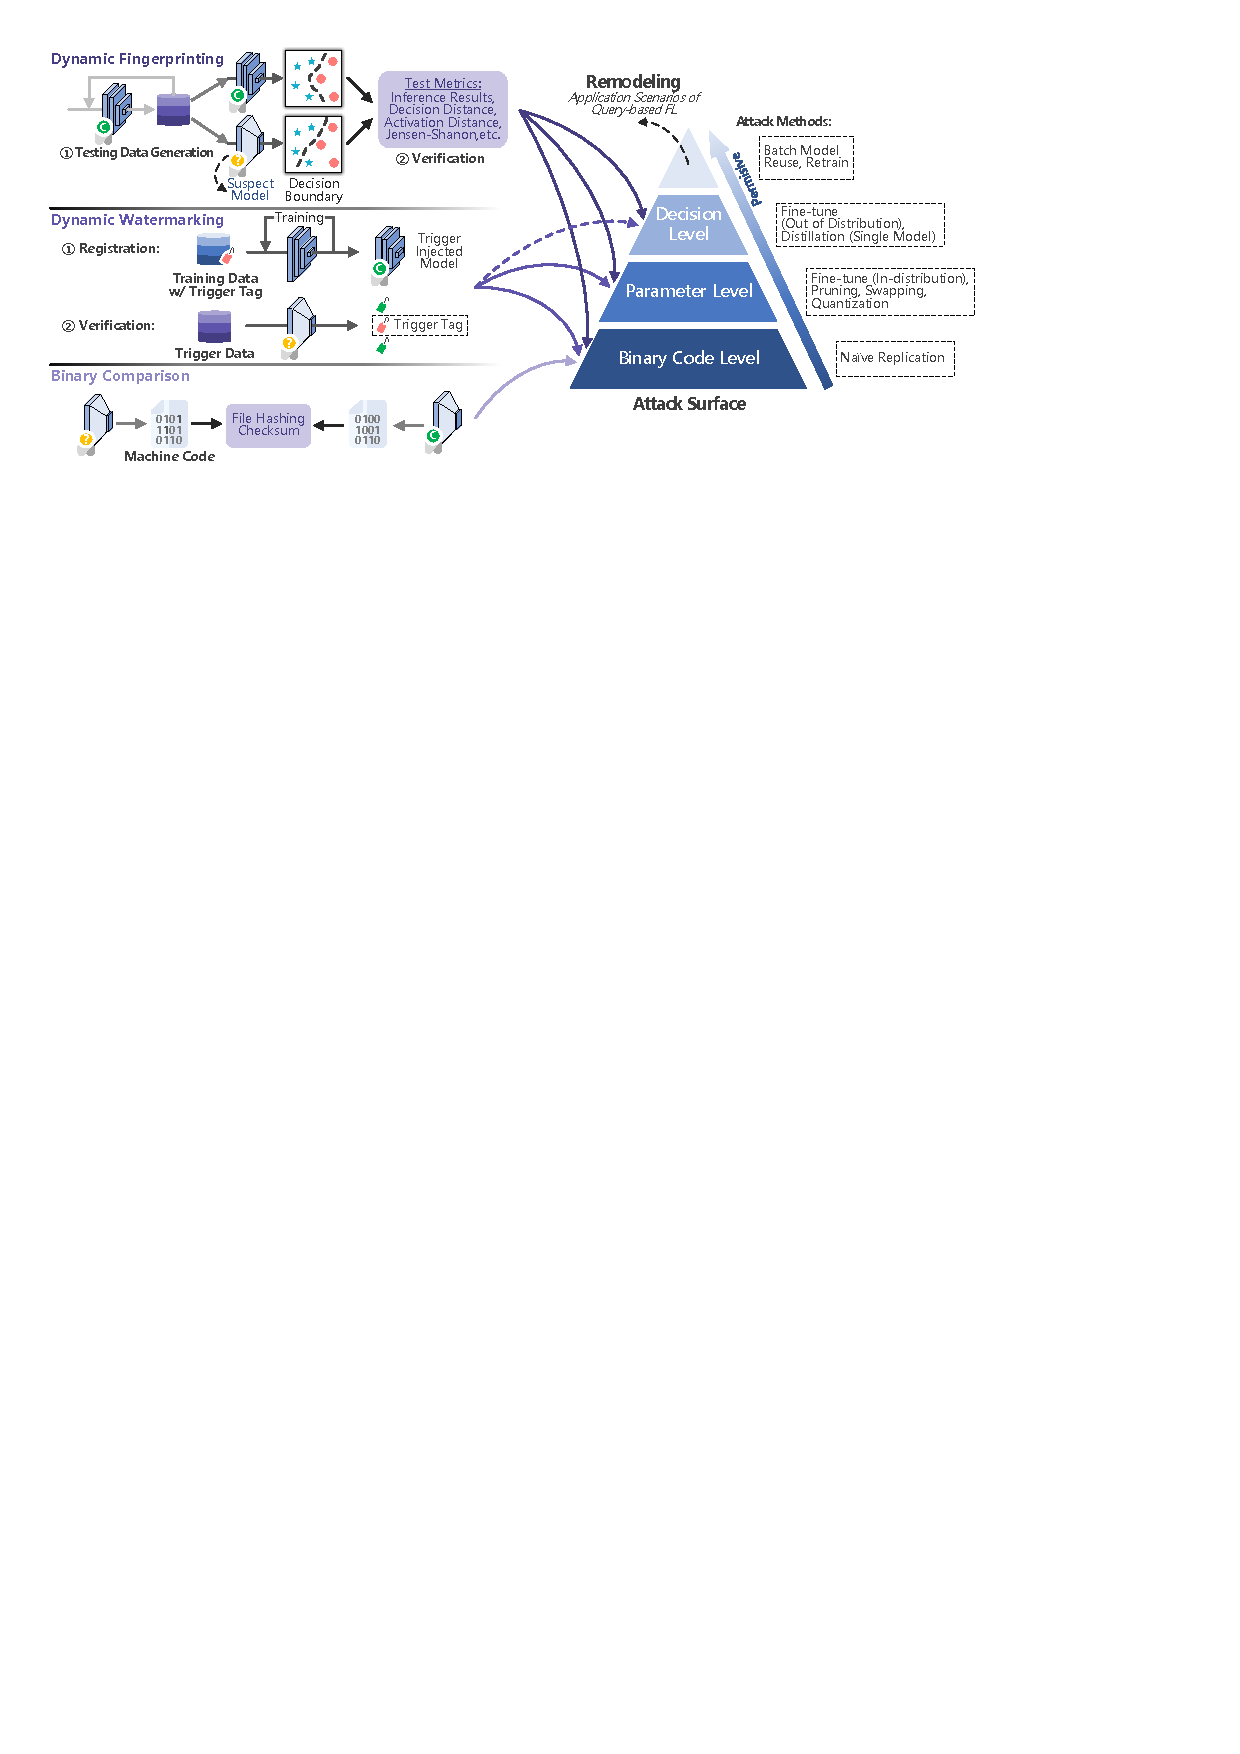
\includegraphics[width=\linewidth]{fig/ip_protection.pdf}
  \caption{Overview of DNNs IP protection methods.}
  \Description{}
  \label{fig:ip}
\end{figure}

In the previous sections, we have extensively discussed the construction of a query-based FL platform from both technical and legal perspectives. 
Nonetheless, the matter of model management and protection continues to be a significant concern, raising questions such as \textit{How can I protect my models from plagiarism after they are released?}
In general, there are three kinds of mechanisms that can be employed to protect DNN models: authorization~\cite{hanzlik2021mlcapsule}, watermarking~\cite{tekgul2021waffle}, and fingerprinting~\cite{li2023fedipr}.
Authorization mechanisms, including hardware-based memory encryption techniques like TEE, can effectively prevent unauthorized access to the model copy.
Additionally, researchers have explored embedding authorization mechanisms within the DNN architecture itself, such as with passport layers~\cite{fan2019rethinking, zhang2020passport}.
However, the need for specific hardware and modifications to model architectures can significantly increase the barriers for participants and compromise the openness of query-based FL platforms.

As passive protection methods, watermarking and fingerprinting can detect potential infringement while preserving the openness of the model. 
A watermark can be embedded into DNNs through training or fine-tuning with a modified loss function~\cite{uchida2017embedding} or trigger data~\cite{darvish2019deepsigns} acting as a backdoor~\cite{bagdasaryan2020backdoor}.
On the other hand, fingerprinting strategies aim to generate an identifier for each model based on snapshots of training history~\cite{jia2021proof} or inference results that approximate decision boundaries~\cite{chen2022copy}.
Note that the technical details of IP protection methods are beyond the scope of this survey.
We recommend referring to up-to-date surveys such as~\cite{peng2022intellectual, sun2023deep}.
Additionally, it is important to recognize that the goal of query-based FL platforms is not to provide perfect protection against model plagiarism and unauthorized use.
Interestingly, certain model reusing strategies like KD and ensemble methods are even regarded as model extraction attacks within the realm of DNNs IP protection~\cite{charette2022cosine}.
This highlights the inherent contradiction between promoting model reusing and preventing all forms of model plagiarism.
As a result, it is necessary to determine the scope of protection and strike a balance between model protection and platform openness.

First, it is helpful to consider the following requirements for model protection in the context of query-based FL:
\begin{itemize}
  \item \textbf{Non-invasive}. Any attempt to invasively embed backdoors into the weights and architectures of models is likely to result in changes to their functionalities and could lead to unexpected failures after deployment~\cite{chen2022copy}. 
  Meanwhile, these backdoors can be exploited by attackers to manipulate the model's predictions~\cite{li2022untargeted}.
  Accordingly, it is more recommend leaving the decision of adding invasive protection to the users instead of forcing it through platforms.
  
  \item \textbf{Compatible}. %模型未知
  Due to the model agnostic nature of query-based FL, relying on protection mechanisms that are specific to certain model structures and formats will limit the applicability of the platform.
  For instance, the passport layer~\cite{zhang2020passport} is built upon the normalization layer and requires joint training with the target model for ownership verification.
  However, in practice, both the normalization layer and whitebox access to the model may be unavailable.
  Therefore, considering the compatibility of model protection mechanisms is essential to ensure wide support for model sharing in query-based FL.

  \item \textbf{Permissive}. % 不对任何行为都检测
  As mentioned earlier, it is not essential to identify and address every instance of plagiarism in query-based FL. 
  On the contrary, we encourage platform users to engage in model mining and reusing, as outlined in Section~\ref{sec:taxonomy}. 
  Therefore, model protection methods should be permissive enough to allow for model reusing while still identifying the less creative effort operations that result in minimal or no change to the model's functionality, such as naive replication, quantization, pruning, and invariant neural swapping.
  Note that the presence of sufficient human creative effort is an important criterion for determining the copyrightability of a computer-generated work~\cite{national1979final}.
  The consideration of copyrightability can serve as a guiding principle in determining the scope of model protection in query-based FL.

  \item \textbf{Large-scale cost-effective}.
  Unlike traditional FL, where the size of training networks in each round is fixed, the size of a query-based FL platform is continuously expandable. 
  Therefore, it is undesirable if the potential conflicts~\cite{li2023fedipr}, required bit-length, and deployment cost~\cite{uchida2017embedding, darvish2019deepsigns} of model protection solutions such as watermarking and fingerprinting increase with the platform size.
  This suggests that solutions that require modifying optimization goals and training or fine-tuning with trigger data to embed identity information into the target model should be excluded.

\end{itemize}

Recently, several model protection algorithms have been proposed to address the challenge of model protection in FL. 
Tekgul \textit{et al.}~\cite{tekgul2021waffle} propose WAFFLE that uses augmented Gaussian noisy images as a watermark set to determine the ownership of the global model. 
However, this method is invasive and incurs high costs due to multiple rounds of training.
To ensure reliable watermarking for FL participants, FedIPR~\cite{li2023fedipr} embeds different watermarks into models of different participants through training with additional trigger samples and a modified optimization goal.
But this method is designed for model verification on the client-side, so it is independent to the model management in FL platforms.
FedTracker~\cite{shao2022fedtracker} embeds personalized local fingerprints into the Batch Normalization (BN) layer to enable traceability of model leakers.
One limitation of FedTracker is that its fingerprinting strategies are not compatible with other DNNs that do not use BN or do not provide whitebox access.
These examples highlight the incompatibility between the IP protection methods designed for traditional FL and the requirements of the query-based FL scenario, which have different protection goals and targets.

Based on the above observation and the taxonomy of deep IP protection~\cite{peng2022intellectual, sun2023deep}, \textbf{dynamic fingerprinting strategies with blackbox verification support} are considered suitable model protection methods for query-based FL.
These methods aim to approximate the similarities between the decision boundaries of different models by evaluating the value of a well-tailored testing metric on a self-constructed testing set.
A typical example is DeepJudge~\cite{chen2022copy}, which employs an ensemble of multi-level (Property, Neuron, Layer) testing metrics to achieve confident and robust plagiarism identification. 
The verification process of DeepJudge can be evaluated in a blackbox setting by calculating distances based on model predictions.
However, the generation of testing set in DeepJudge requires whitebox access to the suspect models in order to calculate adversarial samples, which may be unreachable if the suspect models are in binary format.

Another example is Zest~\cite{jia2022zest}, which randomly samples several training images and then applies super-pixel and segmentation techniques to construct the testing set.
However, this testing samples generation method is limited to images and may expose private training data.
A compromise approach is to seek non-sensitive or desensitized testing set from users when they upload their models.
Inspired by DeepJudge, we can develop an ensemble of multi-level testing strategies for query-based FL.
In the first step, we can compare the hash codes (e.g. MD5, SHA-256) of the raw model weights or its binary execution to rapidly filter out cases of naive replication plagiarism.
Then, in the second step, we can filter out cases of quantization or invariant neural swapping plagiarism by comparing the distance in predictions obtained from an out-of-distribution dataset.
In addition, we can further evaluate the similarities between models using testing-based approaches such as DeepJudge and Zest, which can detect cases of pruning and direct KD plagiarism.
Furthermore, if the workflow information is supports it, we can swiftly eliminate batch model reusing from being suspected of plagiarism.
To enhance understanding, we present an overview of the typical methods used for protecting IP of DNNs in Fig.~\ref{fig:ip}.

In summary, finding a balance between model protection and platform openness is indeed a challenge.
It is crucial to carefully consider the trade-offs and explore alternative approaches that can provide a reasonable level of model protection without excessively compromising the openness and usability of query-based FL platforms.

\begin{comment}
we pre-compute the threshold k based on
the training data and the owner model, which is the maximum
value (upper bound) of the corresponding neuron output over
all training samples.

The reality is that it is not possible to completely prevent all attempts of model plagiarism through technical means, similar to other forms of plagiarism in the realm of intellectual property. However, the good news is that it is not essential to identify and address every instance of plagiarism.
Finding a balance between model protection and platform openness is indeed a challenge.
It is crucial to carefully consider the trade-offs and explore alternative approaches that can provide a reasonable level of model protection without excessively compromising the openness and usability of query-based FL platforms.

passive

~\cite{chen2022copy}
barrier~\cite{peng2022intellectual}
\end{comment}





% 分为feature-based 和 Backdoor-based 两种
% 重点讨论哪些方法适用于query-based FL,要求:由server添加和校验,尽量不依赖隐私数据和重新训练,尽量不影响模型性能,支持blackbox
% 现在的IP protection方法不能提供百分白的判断,没有形成技术的标准.
% Will releasing this make it easy for my main competitor to copy this new feature and hurt our differentiation in the market?
%  they were most worried about competitors gaining an advantage from what we released.because modern machine learning has become essential for many applications
% Fictitious or fake entries are deliberately incorrect entries in reference works such as dictionaries, encyclopedias, maps, and directories, added by the editors as a copyright trap to reveal subsequent plagiarism or copyright infringement. There are more specific terms for particular kinds of fictitious entry, such as Mountweazel, trap street, paper town, phantom settlement, and nihilartikel
%query-based FL只需要判定小程度的相似,而不需要对KD和retrain这类进行判断。可以把对篡改行为的检测划分为几个等级:1)bit-wise的修改(任何篡改行为);2)参数的修改,基本不改变判别边界;3)模型结构的修改,基本不改变判别边界;4)模型结构的修改,基本不改变判别边界(剪枝,量化)5)重新训练,基于相同数据集但是不同随机种子,通过workflow来判别-----》其实我们只需要识别是否判别边界明显改变了
% 事实上,model reusing 也是一种攻击IP的方法,与传统FL不同,相反的,我们欢迎对模型的再次利用,并且复用和IP保护其实是存在冲突的。
% While in DNN watermarking, besides the static content, such as the model parameters and architectures, the owner can also embed the watermark into the model’s functionality, referred to as the dynamic content.
% non-invasive

\begin{comment}
  File Hashing: Generate a hash value for each binary code using a hashing algorithm such as MD5, SHA-1, or SHA-256. Compare the hash values of the two binary codes. If the hash values are identical, it indicates that the binary codes are the same.
Binary Comparison Tools: Use specialized software tools designed for binary file comparison. These tools analyze the binary codes at the byte level and provide a detailed comparison report highlighting any differences between the files.
Binary Diffing: Perform a binary diffing process, which involves comparing the two binary codes at the assembly or machine code level. This method is typically used for analyzing differences in code or reverse engineering purposes.
Checksum Comparison: Compute a checksum for each binary code using a checksum algorithm such as CRC (Cyclic Redundancy Check). Compare the checksum values of the two binary codes. If the checksums match, it indicates that the binary codes are the same.
\end{comment}

\section{Contract-based Federated Learning}
\label{sec:contract}
Let us consider another open FL platform based on a contract-based cooperation framework, where cooperation can be built by publishing ML tasks and accepting ML collaboration requests.
An overview of this platform is presented in Fig.~\ref{fig:contract}, the major difference between traditional FL (ref Fig.~\ref{fig:fl}) and contract-based FL is that we involve a trustworthy third-party platform called the Contract Platform to host and coordinate ML tasks for platform users.
Rather than directly pushing ML tasks from servers to clients, employers need to publish the tasks to the contract platform and wait for acceptance from workers, which involves a mutual choice procedure. 
The conditions and payment for participation are also appliable, and the final model will be audited and evaluated by the platform for fairness.
In addition, privacy-enhanced technologies~\cite{hesamifard2018privacy} and fingerprint management~\cite{chen2022copy} can also be implemented by the platform to protect the IP of platform users.
The properties of contract-based FL are: 1) \textbf{Opt-in}, as workers reserve the right to join or quit from training networks; 2) \textbf{Contractual}, enabling employers to define payment, organization mode, model quality criteria, rehire rules, etc. through contracts; 3) \textbf{Market-based}, where contracts are open and task pricing is influenced and determined by the market.

\begin{figure}[t]
    \centering
    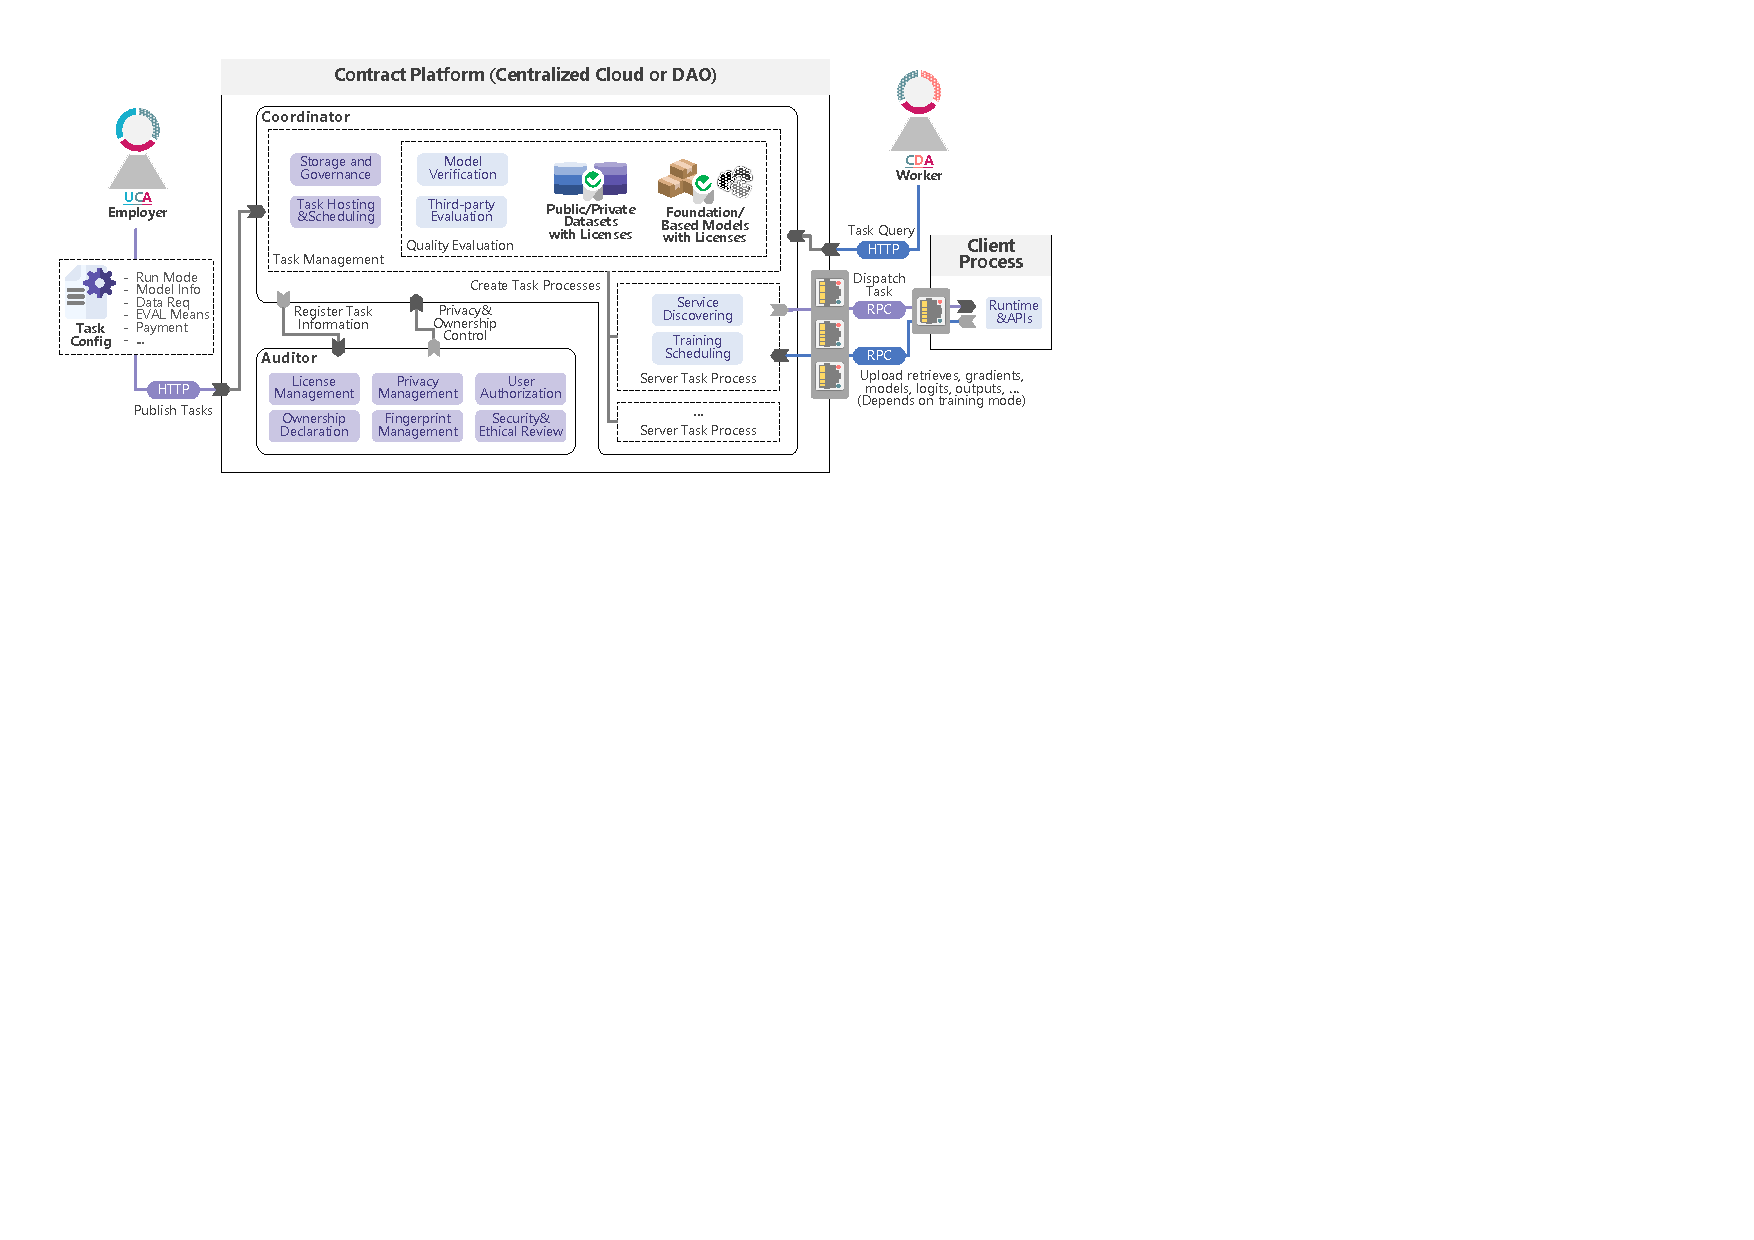
\includegraphics[width=\linewidth]{fig/contract_frame.pdf}
    \caption{An overview of contract-based FL systems. (U: model User, C: Coordinator, D: Data owner, A: Auditor)}
    \Description{}
    \label{fig:contract}
\end{figure}

In short, contract-based FL retains all functionalities related to model training at the platform and only provides task publishing services to employers, who play the role of model training in traditional FL.
Furthermore, similar to model-reusing mechanisms (ref. Section~\ref{sec:taxonomy}) that can be applied to query-based FL, our contract-based FL is not limited to an amalgamation-based collaborative training paradigm like FedAvg.
In fact, the contract platform is designed as a crowdsourcing platform among data miners for ML cooperation tasks, including distributed training, fine-tuning, and ensembling based on scratch or Foundation Models (FMs)~\cite{yuan2022decentralized}.
However, most current crowdsourcing platforms like Amazon Mechanical Turk\footnote{https://www.mturk.com/} and Appen\footnote{https://appen.com/crowd-2/} primarily deal with human intelligence tasks such as data collection and annotation (aka microtasks) rather than ML modeling tasks. 
It remains unexplored how to design and publish an ML task to seek crowd labor.
On the other hand, many studies~\cite{dias2022blocklearning, blythman2022decentralized, deng2021flex, guo2023blockchain, batool2022fl} and products~\cite{steeves2022incentivizing, ziller2021pysyft, mcconaghy2022ocean} emphasize monetizing ML activities through blockchain-based techniques and Decentralized Autonomous Organizations (DAOs). 
However, both monetization and decentralization are non-essential functions for our contract platforms, and we will summarize and compare these works later.


\subsection{How to Design ML Microtasks}

When we come to the scenario of contract-based FL, we first need to define how to design ML microtasks for crowd workers. 
Unfortunately, previous collaborative ML studies~\cite{li2021survey, nguyen2021federated} rarely discuss this question because they default to assuming that all employers or workers have the same resource type to fit into their modeling frameworks.
On the contrary, in contract-based FL, we leave the freedom of design microtasks and choosing modeling method to the employers.

The answer to this question depends on what resources the employers have and what tasks the workers can perform.
For example, in horizontal FL, the server should provide an initial model, and clients should have training data under the same feature space and provide computational power. However, in vertical FL, the clients should have training data under the same sample space (i.e., ID space). 
This difference determines which modeling framework employers can adopt. 
Following this idea, we provide comparisons of typical FL, distributed ML, and blockchain-based modeling frameworks in Table~\ref{tab:train}.
For simplicity, we introduce the \textbf{Platform} between Employer and Worker in some frameworks to make it adaptable for contract-based FL. 
You can quickly restore the original structure by merging Employer and Platform columns.
To represent the transmission of resources, we mark resources provided by each group of entities with different colors.
The computational resource used for training is marked with $\bigstar$.
By this way, we can conveniently find the feasible and privacy-preserving modeling frameworks for collaborative learning. 
Here, we briefly introduce these frameworks group by scenarios\footnote{From the viewpoint of Employers.}.

\subsubsection{Train from scratch with workers' private data}
There are four frameworks that support this scenario. 
The first is \textbf{Centralized ML}, which requires workers to upload their data to a cloud platform for modeling. However, this approach is not feasible for FL scenarios due to privacy concerns. 
The second is \textbf{FedAvg}~\cite{mcmahan2017communication}, which requires workers to upload computed gradients upon the scratch model and their private data (horizontally split). Computing resources need to be provided by workers as well.
The third is \textbf{SplitNN}~\cite{vepakomma2019split}, where each worker trains the cut layers of the model using their vertically split data. 
The hidden representations from these layers are uploaded to the platform for the training of the remaining layers.
The last and distinctive is a Web3 system named \textbf{Ocean}~\cite{mcconaghy2022ocean}.
It enables workers to upload only the metadata of their local dataset to a blockchain-based platform to attract buyers. 
Interested buyers then need to purchase datatokens to access the local dataset and deploy their modeling algorithm. 
To ensure the privacy and IP security of workers, only trusted algorithms are allowed, and only model predictions will be sent to buyers.

\begin{table}[t]
    \centering
    \small
    \caption{Comparisons of typical model training frameworks with the intervention of a trustworthy platform. \colorbox{Employer!30}{\textasteriskcentered}, \colorbox{Platform!30}{\textasteriskcentered}, \colorbox{Worker!30}{\textasteriskcentered} indicate resources from \colorbox{Employer!30}{Employer}, \colorbox{Platform!30}{Platform}, and \colorbox{Worker!30}{Worker}, respectively. Resources in different color columns (e.g., \colorbox{Worker!30}{Data} in column \colorbox{Platform!30}{Platform}) represent transmission. $\bigstar$: Location of model training. \colorbox{Worker!30}{\textit{Resources}} received from other workers.}
    \label{tab:train}
    \begin{tabular}{|l|p{2.6cm}|p{4cm}|p{5cm}|}
    \hline
    & \multicolumn{1}{c|}{\cellcolor{Employer!30}{Employer}} & \multicolumn{1}{c|}{\cellcolor{Platform!30}{Platform}} & \multicolumn{1}{c|}{\cellcolor{Worker!30}{Worker}} \\ \hline
    
    Centralized ML & \colorbox{Employer!30}{Model} & \colorbox{Employer!30}{Model}\colorbox{Worker!30}{Data} $\bigstar$ & \colorbox{Worker!30}{Data} \\ \hline %Scratch

    FedAvg~\cite{mcmahan2017communication} & \colorbox{Employer!30}{Model} & \colorbox{Employer!30}{Model}\colorbox{Worker!30}{Gradient} & \colorbox{Employer!30}{Model}\colorbox{Worker!30}{Data} $\bigstar$ \\ \hline %Scratch

    DMoE~\cite{ryabinin2020towards} & \colorbox{Employer!30}{Gating NN}\colorbox{Employer!30}{Data} & \colorbox{Employer!30}{Gating NN}\colorbox{Employer!30}{Data}\colorbox{Worker!30}{Output} $\bigstar$ & \colorbox{Worker!30}{Model}\colorbox{Employer!30}{Data} $\bigstar$ \\ \hline %Scratch

    DeDES~\cite{wang2023data} & \colorbox{Worker!30}{Model Subset} & \colorbox{Worker!30}{Model} & \colorbox{Worker!30}{Model}\colorbox{Worker!30}{Data} $\bigstar$ \\ \hline %Scratch
    
    Borzunov \textit{et al.}~\cite{borzunov2022training} & \colorbox{Employer!30}{Model} & \colorbox{Employer!30}{Model}\colorbox{Platform!30}{Data}\colorbox{Worker!30}{Gradient} & \colorbox{Employer!30}{Model}\colorbox{Platform!30}{Data-Stream} $\bigstar$ \\ \hline %Scratch, DHT

    Moshpit SGD~\cite{ryabinin2021moshpit} & \colorbox{Employer!30}{Model}\colorbox{Employer!30}{Data} & \colorbox{Employer!30}{Model}\colorbox{Employer!30}{Data}\colorbox{Worker!30}{Gradient} & \colorbox{Employer!30}{Model}\colorbox{Employer!30}{Data-Loader} $\bigstar$ \\ \hline 

    VC-ASGD~\cite{atre2021distributed} & \colorbox{Employer!30}{Model}\colorbox{Employer!30}{Data} & \colorbox{Employer!30}{Model}\colorbox{Employer!30}{Data}\colorbox{Worker!30}{Gradient} & \colorbox{Employer!30}{Sub-model}\colorbox{Employer!30}{H-Data} $\bigstar$ \\ \hline

    SplitNN~\cite{vepakomma2019split} & \colorbox{Employer!30}{Model}\colorbox{Employer!30}{ID-Label} & \colorbox{Employer!30}{Model}\colorbox{Employer!30}{ID-Label}\colorbox{Worker!30}{Hidden} $\bigstar$ & \colorbox{Employer!30}{Sub-model}\colorbox{Worker!30}{V-Data}\colorbox{Platform!30}{Gradient} $\bigstar$ \\ \hline
    
    DT-FM~\cite{yuan2022decentralized} & \colorbox{Employer!30}{FM} & \colorbox{Employer!30}{FM}\colorbox{Platform!30}{Data} & \colorbox{Employer!30}{Sub-FM}\colorbox{Platform!30}{Micro-Batch}\colorbox{Worker!30}{\textit{Gradient}} $\bigstar$ \\ \hline

    FS-LLM~\cite{kuang2023federatedscope} & \colorbox{Employer!30}{FM} & \colorbox{Employer!30}{FM}\colorbox{Worker!30}{Adapter} & \colorbox{Employer!30}{FM}\colorbox{Worker!30}{Data} $\bigstar$ \\ \hline

    FedKSeed~\cite{qin2023federated} & \colorbox{Employer!30}{FM} & \colorbox{Employer!30}{FM}\colorbox{Platform!30}{Seed}\colorbox{Worker!30}{Scaler Gradient} & \colorbox{Employer!30}{FM}\colorbox{Platform!30}{Seed}\colorbox{Worker!30}{Data} $\bigstar$ \\ \hline

    Berdoz \textit{et al.}~\cite{berdoz2022scalable} & \colorbox{Employer!30}{Class} & \colorbox{Employer!30}{Class}\colorbox{Platform!30}{NN Structure}\colorbox{Worker!30}{Hidden} & \colorbox{Platform!30}{NN Structure}\colorbox{Worker!30}{Data}\colorbox{Platform!30}{Hidden AVG} $\bigstar$ \\ \hline

    CCL~\cite{aketi2024cross} & \colorbox{Employer!30}{Class} & \colorbox{Employer!30}{Class} & \colorbox{Worker!30}{Data}\colorbox{Worker!30}{\textit{Model}}\colorbox{Worker!30}{\textit{Hidden AVG}} $\bigstar$ \\ \hline

    FedProto~\cite{tan2022fedproto, michieli2021prototype} & \colorbox{Employer!30}{Class} & \colorbox{Employer!30}{Class}\colorbox{Worker!30}{Hidden} & \colorbox{Worker!30}{Data}\colorbox{Worker!30}{Model}\colorbox{Platform!30}{Hidden AVG} $\bigstar$ \\ \hline   

    Ocean~\cite{mcconaghy2022ocean} & \colorbox{Employer!30}{Model}\colorbox{Worker!30}{Output} & \colorbox{Worker!30}{Metadata} & \colorbox{Worker!30}{Metadata}\colorbox{Employer!30}{Model}\colorbox{Worker!30}{Data} $\bigstar$ \\ \hline

    \end{tabular}
\end{table}

\subsubsection{Ensemble workers' private model} %优点:支持模型异构
As we presented in Section~\ref{sec:taxonomy}, ensembling is an effective method to integrate knowledge, and the distributed version is proposed by \textbf{DMoE}~\cite{ryabinin2020towards}. 
It employs a Distributed Hash Table (DHT) to store metadata and worker node statuses, constructing a decentralized expert network. 
To make inferences using this network, each model user must train a local gating network to select a subset of experts tailored to their input.
No additional training required, Wang \textit{et al.} purposed \textbf{DeDES}~\cite{wang2023data}, which selects a diverse subsect of weak models from population and make inference by voting. 
The unique advantage of ensembling lies in its inherent support for model heterogeneity, and its integration is extensible. 
This capability enables the establishment of a cooperative network while maintaining flexibility and availability.

\subsubsection{Train from fundation model}
Foundation models, trained on larger-scale data with robust generalization abilities across various downstream tasks, serve as a solid foundation for collaborative training. 
Yuan \textit{et al.} proposed \textbf{DT-FM}~\cite{yuan2022decentralized} to establish an effective geo-distributed learning system across 8 regions for training the language model GPT-3.
Similarly, Borzunov \textit{et al.}\cite{borzunov2022training} recruited volunteer nodes to train a transformer model over the Internet. 
To enhance system robustness, \textbf{Moshpit SGD}~\cite{ryabinin2021moshpit} divides worker nodes into small, independent groups to ensure that all-reduce is not affected by the failure of a single participant.
Additionally, \textbf{VC-ASGD}\cite{atre2021distributed} divides the deep learning training job into asynchronous parameter update subtasks to improve scalability.
In these cases, employers are required to supply the initial model and training data needed to launch training subtasks. 
This training paradigm is particularly suitable for worker nodes that possess computational and communication resources but lack their own training data.

Instead of initiating training from scratch and consuming substantial computational resources, we can also collaboratively adapt these foundation models to specific local tasks based on relatively restricted hardware and data size through fine-tuning.
Recently, Woisetschl{\"a}ger \textit{et al.}~\cite{woisetschlager2023federated} have explored the opportunity to fine-tune large language models, such as FLAN-T5, by edge devices.
Simultaneously, \textbf{FS-LLM}~\cite{kuang2023federatedscope} employs Parameter-Efficient Fine-Tuning (PEFT) methods for federated fine-tuning of LLaMA-7B, minimizing communication and computation costs.
\textbf{FATE-LLM}~\cite{fan2023fate} offers a solution called FedHeteroLLM, leveraging KD to train a mentee model from its local pre-trained LLM for federated aggregation.
To alleviate the computational burden associated with backpropagation-based optimization methods, \textbf{FedKSeed}~\cite{qin2023federated} employs zeroth-order optimization (ZOO). 
Only seed and scalar gradients need to be transmitted for federated fine-tuning.

\subsubsection{Representations Sharing}
Another popular scheme for organizing ML microtasks involves sharing the learned representations of workers. 
For instance, the use of class-conditional average of last hidden layer activations (aka. Prototypes) can enhance class discrimination across different clients~\cite{aketi2024cross, tan2022fedproto, michieli2021prototype, berdoz2022scalable}.
To configure the microtasks, employers only need to set the target class, after which the platform can collect and distribute per-class prototypes among workers.
With no central server required, \textbf{CCL}~\cite{aketi2024cross} presents a decentralized learning approach based on cross-workers prototypes sharing.
%However, the choosing between central solution and decentral solution is depends on what kind of infrastructure are perfered.
%For example, we can decentralized the store of local mode by IPFS~\cite{benet2014ipfs} protocol

\subsection{Decentralization and Monetization}
Parallel to contract-based FL, several efforts are underway to build decentralized AI platforms through Web3-based techniques~\cite{guo2023blockchain}. 
For instance, Blythman \textit{et al.} proposed decentralized AI Hubs~\cite{blythman2022decentralized}, empowered by DAOs (e.g., IPFS~\cite{benet2014ipfs}, Ocean~\cite{mcconaghy2022ocean}, OpenMined), to run ML activities in a trustless setting.
Wickstr{\"o}m \textit{et al.}~\cite{wickstrom2022decentralizing} propose the concept of AI market which builds a ML analysis network for IoT devices based on Ethereum.
Similar to DMoE, Bittensor~\cite{steeves2022incentivizing} encapsulates neural network models as services and rewards peers contributing information-theoretic value to the system with TAO coins. 
Remote peers can be reused, for example, in the form of a MoE, or they can be pipelined to a new service.

The advantages of these blockchain-based systems are that transactions are transparent and workers can easily be incentivized.
Therefore, it is a solution when it is challenging to establish a trust relationship between platform users. 
However, if available, we can replace these DAOs' infrastructural components with a trusted crowdsourcing platform.
Like Amazon Mechanical Turk, the incentivized mechanisms is no nessary for contract-based FL platforms as the rewards are set by employers in contract.
While many studies consider Shapley value to evaluate the contribution of clients in FL systems~\cite{zhan2021survey}, we emphasize that a third-party evaluation can also be conducted in a crowdsourcing manner.
Similarly, as the model community in query-based FL, contract platforms can further provide IP protection services to users (ref. Section~\ref{sec:how2protect}). 
Dynamic fingerprints of models can be recorded and used for plagiarism detection.
Three kinds of interests should be considered: 1) Interest of employers, to prevent the information leakage of task configurations; 2) Interest of workers, requiring fair evaluation of labor; 3) Interest of the public, to curb the infringement of privacy.
However, this is not only a challenge from a technical perspective but also necessitates corresponding legislative oversight to provide guidelines to standardize this kind of AI marketplace commercialization.
We believe that a comprehensive regulatory framework is essential to ensure data privacy, and establish fair practices in the evolving landscape of open FL platforms.

\subsection{Limitations of Contract-based FL}
In contract-based FL systems, employers can publish their personalized ML crowdsourcing tasks, considering both their local resources and the resources of the target clients. 
However, to meet the flexibility requirements of widely supporting training methods, the contract platform should offer highly compatible APIs that can integrate various distributed training frameworks. 
Additionally, it needs to provide comprehensive audit against malicious users and plagiarism, significantly increasing the complexity compared to traditional FL and query-based FL.
Meanwhile, to establish confidence among users, a fair and consensual third-party model evaluation mechanism should be established, which, however, is almost unexplored in the current academic studies.

\begin{comment}
In query-based FL systems, the processes of model production and reuse are decoupled to maximize the autonomy of each participant. 
However, this losse cooperation paradigm is no longer compatiable with online collaboration ML frameworks, which means that it cannot fully harness participants' communicational and computational resource to enhace the training performance.
Therefore, even though the server-dominated cooperation frameworks like FedAvg have limitations, as described in Section~\ref{sec:limitations_FL}, it is still worthwhile to provide support for its underlying distributed ML training methods to enhance the flexibility and compatibility of our open FL platforms.
In the next section, we illustrate another cooperation framework named contract-based FL, which follows a mutual choice design philosophy similar to crowdsourcing platforms~\cite{vaughan2018making}.
It can serve as an extension of traditional FL and query-based FL.
\end{comment}


\section{Conclusion}
Traditional federated learning systems with a server-dominated cooperation framework suppress the enthusiasm of participants and limit the further extension of such collaboration. 
To explore the opportunity to establish a more open and reciprocal cooperation platform, we investigate current progress in federated learning, decentralized machine learning, and model reusing systems. 
In this way, we depict two rough sketches of open federated learning platforms: query-based federated learning paltform and contract-based federated learning paltform. 
Based on these two proposed platforms, we survey their possible supported techniques and their related legal issues, including ML licensing and copyrightability. 
We believe this survey can encourage a rethinking of current collaborative ML systems design and lead to the pervasive availability of AI for everyone.


%Therefore, we don't delve into this topic in this survey.

% 目标:1)保护任务发布方的利益和隐私;2)保护数据所有者的利益和隐私;3)遏制侵权行为

% 如何衡量模型质量:1)第三方evaluation

% 如果不采用pipeline的方式训练,如何拆分训练任务?

% 如何发现可用的FL节点
% 几种训练组织方式


%%
%% The acknowledgments section is defined using the "acks" environment
%% (and NOT an unnumbered section). This ensures the proper
%% identification of the section in the article metadata, and the
%% consistent spelling of the heading.
\begin{acks}

\end{acks}

%%
%% The next two lines define the bibliography style to be used, and
%% the bibliography file.
\bibliographystyle{ACM-Reference-Format}
\bibliography{REF}


%%
%% If your work has an appendix, this is the place to put it.
\appendix

\end{document}

\endinput
%%
%% End of file `sample-acmlarge.tex'.
